\message{ !name(main.tex)}\documentclass[12pt,a4paper]{book}
\raggedbottom


% -------------------------------------------------
% Diseño de capítulos y secciones
% -------------------------------------------------

\usepackage{titlesec}
\usepackage{xcolor}

\definecolor{chapterrule}{gray}{0.55}

\titleformat{\chapter}[hang]
  {\sffamily\bfseries\Large}
  {\thechapter}
  {1em}
  {}
  [\vspace{0.5ex}{\color{chapterrule}\titlerule[0.4pt]}]

\titlespacing*{\chapter}
  {0pt}
  {0pt}
  {2.5ex}

\titleformat{\section}
  {\sffamily\bfseries\normalsize}
  {\thesection}
  {1em}
  {}

\titlespacing*{\section}
  {0pt}
  {2.5ex}
  {1ex}

% -------------------------------------------------

\usepackage{ugmath_notas}
\AtBeginDocument{\shorthandoff{<>}} % los atajos «<<»/«>>» de babel-spanish chocan con < y > usados como símbolos matemáticos
\usepackage{float}
\usepackage{placeins}
\usepackage[labelfont=bf,labelsep=space]{caption}
\usepackage{pdfpages}
\usepackage{tikz-cd}
\usepackage{amsthm}
\renewcommand{\Tr}{\operatorname{Tr}}
\newcommand{\llaves}[1]{\{#1\}}
\newcommand{\parentesis}[1]{\left(#1\right)}
\newcommand{\corchetes}[1]{\left[#1\right]}
\newcommand{\llavesgrande}[1]{\big\{#1\big\}}
\newcommand{\llavesgrandes}[1]{\left\{#1\right\}}
\newcommand{\comillas}[1]{"#1"}
\usepackage{booktabs}
\addto\captionsspanish{%
  \renewcommand{\tablename}{Tabla}
}

\newcommand{\HH}{\mathcal{H}}
\newcommand{\GG}{\mathcal{G}}
\newcommand{\VV}{\mathcal{V}}
\DeclareMathOperator{\libre}{libre}
\DeclareMathOperator{\lig}{lig}
\DeclareMathOperator{\Th}{Th}
\DeclareMathOperator{\Mod}{Mod}

% Las figuras (diagramas de resolución, Sección 1.8) viven como fuentes
% standalone externas en figuras/, en la raíz de DEMAT-UG.
\graphicspath{{../../../../figuras/}}

% Entorno para exhibir demostraciones formales en dos columnas
% (afirmación numerada / justificación), al estilo de las
% derivaciones de la Sección 1.4.
\newenvironment{derivacion}{%
  \begingroup
  \renewcommand{\arraystretch}{1.35}
  \begin{center}
  \begin{tabular}{@{}l l@{}}
    \textbf{Afirmación} & \textbf{Justificación}\\
    \hline
}{%
  \end{tabular}
  \end{center}
  \endgroup
}



\begin{document}

\message{ !name(main.tex) !offset(-3) }



    \thispagestyle{empty}
    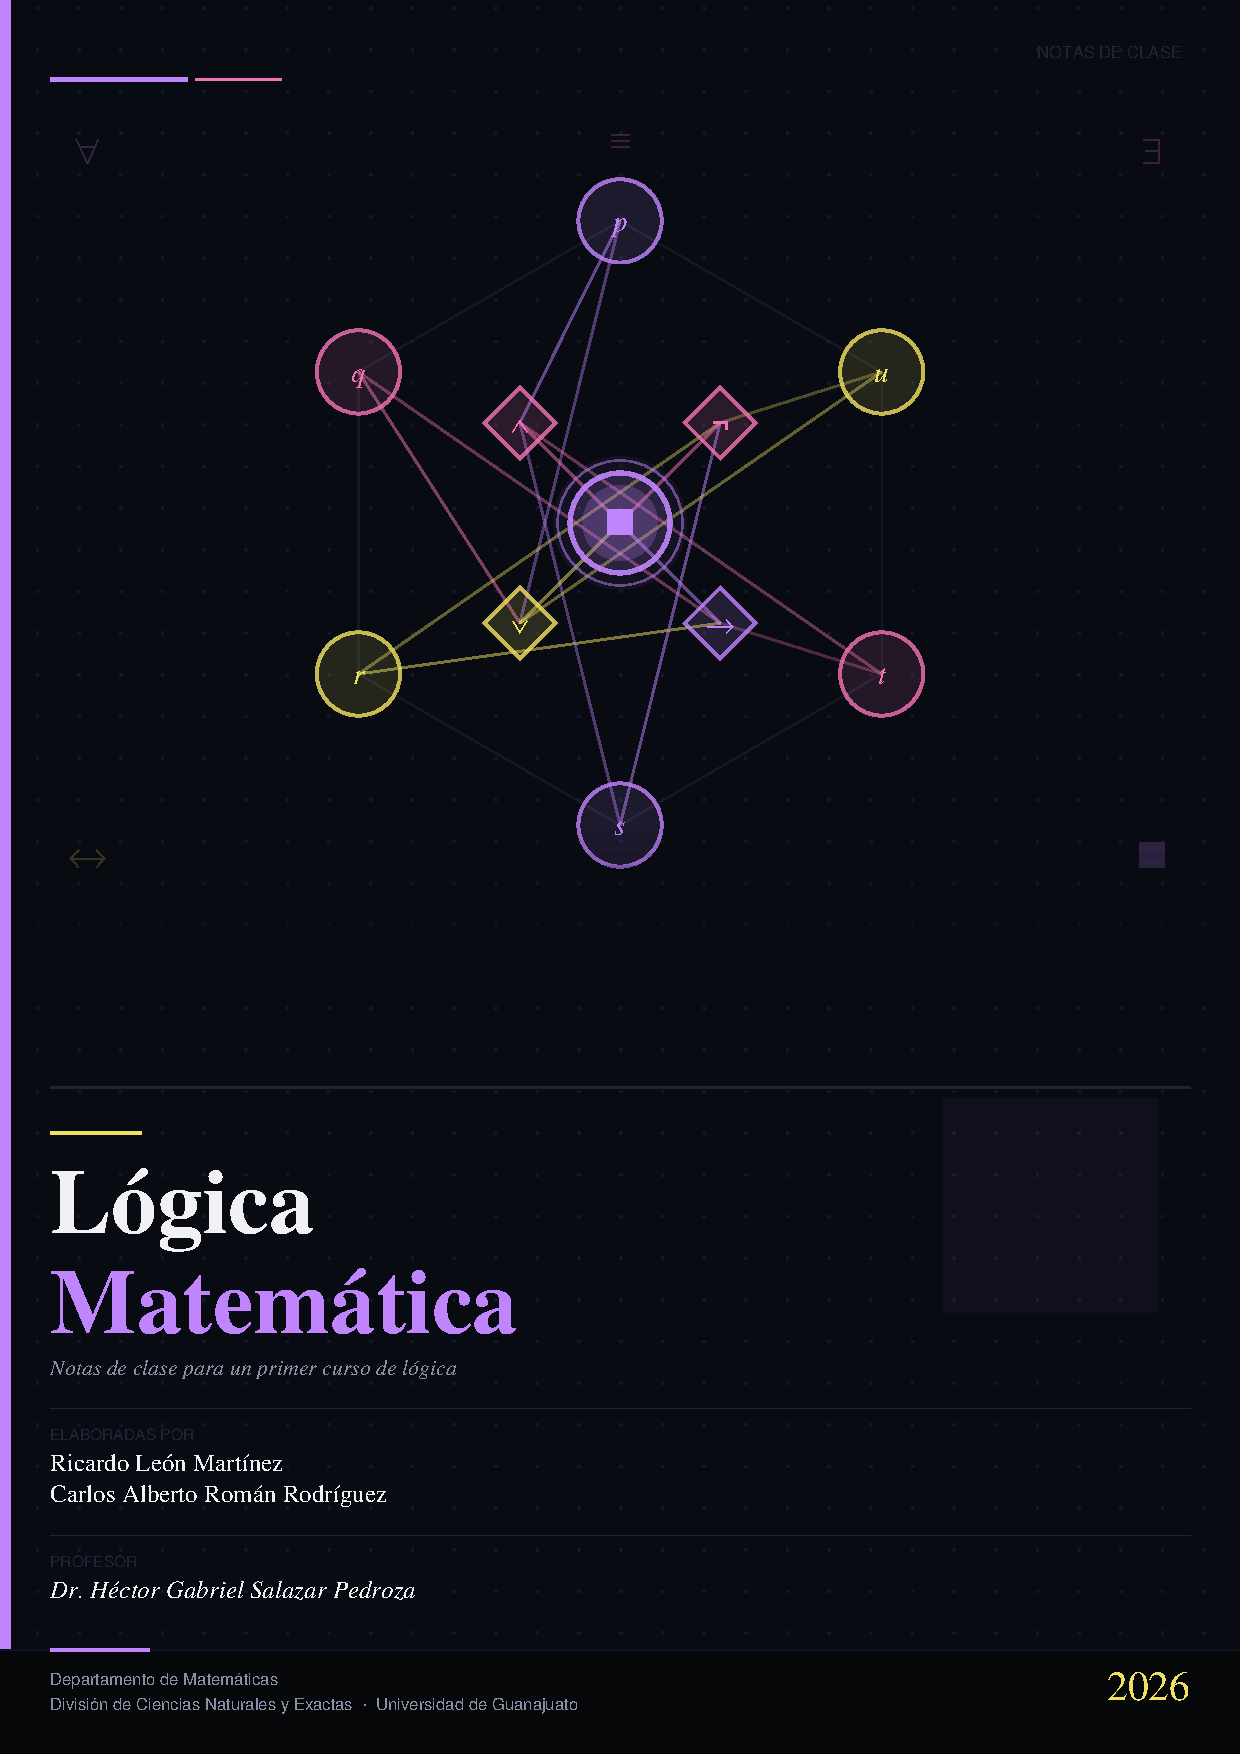
\includepdf[pages=1]{portada_logica_matematica.pdf}

    \begin{flushright}
      \thispagestyle{empty}

        \textbf{Ricardo}\\[0.3cm]

        Aqui son las dedicatorias pero hay que ponerlas hasta el final

        \textbf{Roman}
    \end{flushright}

    % ---------------- NOTA DE ERRORES ----------------

    \cleardoublepage
    \thispagestyle{empty}

    \begin{mdframed}[style=mdgreenbox]
        \begin{center}
        \small
        Estas notas fueron elaboradas con fines académicos.\\
        A pesar del cuidado puesto en su redacción,\\
        es posible que existan errores u omisiones.\\[0.3cm]

        Cualquier corrección, sugerencia o comentario será bienvenido
        en los correos correo: \\[0.3cm]

        ricardo.leon@cimat.mx\\
        carlos.roman@cimat.mx
        \end{center}
    \end{mdframed}

    % -------------------------------------------------

    \setcounter{page}{1}
    \tableofcontents

    \chapter{Lógica Proposicional}

    \section{¿Qué es la lógica proposicional?}

    En lógica proposicional, las fórmulas atómicas son proposiciones. Cualquier afirmación vale. Por ejemplo

    \begin{quote}
        A=\comillas{Aristóteles ha muerto,}\\
        B=\comillas{Barcelona está a orillas del Sena,} y\\
        C=\comillas{Courtney Love es alta}
    \end{quote}

    son fórmulas atómicas. Las fórmulas atómicas son los elementos básicos que se utilizan para construir
    proposiciones. En cualquier lógica, una proposición se considera un tipo concreto de fórmula. En la
    lógica proposicional, no existe distinción entre estos dos términos. Utilizamos \comillas{fórmula} y
    \comillas{proposición} indistintamente.\\
    En la lógica proposicional, al igual que en todas las lógicas que estudiamos, cada proposición es verdadera
    o falsa. A la proposición se le asigna, en consecuencia, un \textit{valor de verdad} de 1 o 0. En el ejemplo anterior, podemos
    asignar el valor de verdad 1 a la fórmula A y el valor de verdad 0 a la fórmula B. Si tomamos la proposición C al pie de la letra,
    su veracidad es discutible. Quizá, tendría más sentido permitir valores de verdad entre 0 y 1. Podríamos asignar un 0,75 a la afirmación C
    si la señorita Love es más alta que el $75\%$ de las mujeres estadounidenses. La lógica difusa permite tales valores de verdad,
    pero las lógicas clásicas que estudiamos no.\\
    De hecho, el contenido de las proposiciones no es relevante para la lógica proposicional. De ahora en adelante, las fórmulas
    atómicas se denotarán únicamente mediante las letras mayúsculas A, B, C,$\dots$ (posiblemente con subíndices) sin hacer referencia a lo
    que estas proposiciones realmente dicen. La veracidad de estas fórmulas no nos concierne. La lógica proposicional no es el estudio de la verdad,
    sino de la relación entre la verdad de una afirmación y la de otra.\\
    El lenguaje de la lógica proposicional contiene palabras como \comillas{no}, \comillas{y}, \comillas{o}, \comillas{implica} y
    \comillas{si y solo si}. Estas palabras se representan mediante símbolos:
    \begin{gather*}
        \neg\text{ para \comillas{no}, }\land\text{ para \comillas{y}, }\lor\text{ para \comillas{o},}\\
        \rightarrow\text{ para \comillas{implica}, }\leftrightarrow\text{ para \comillas{si y solo si}.}
    \end{gather*}

    Como ocurre siempre que se traduce de un idioma a otro, esta correspondencia no es exacta. A diferencia de sus equivalentes en inglés,
    estos símbolos representan conceptos precisos e invariables. El significado de una palabra en inglés, por el contrario, siempre depende
    del contexto. Por ejemplo, $\wedge$ representa un concepto similar, pero no idéntico, a \comillas{y}. Para las fórmulas atómicas
    $A$, $B$ y $A\wedge B$ siempre significa lo mismo que $B\wedge A$. Esto no siempre es así con la palabra \comillas{y}. La oración

    \begin{quote}
        Se puso muy enferma y fue al médico.
    \end{quote}

    no tiene el mismo significado que

    \begin{quote}
        Fue al médico y se puso muy mal.
    \end{quote}

    Del mismo modo, $\vee$ difiere de \comillas{o}. En el lenguaje coloquial, el uso de \comillas{A o B} suele excluir la posibilidad
    de que se den tanto A como B. En lógica proposicional, $A\vee B$ siempre significa o bien $A$, o bien $B$, o bien tanto $A$
    como $B$.\\
    Debemos definir con precisión los símbolos $\neg,\wedge,\vee,\rightarrow\text{ y }\ssi$. Nos enfrentamos
    al dilema de cómo definir la primera de un lenguaje (¡sin recurrir a ninguna otra palabra!). Por este motivo,
    tomamos los símbolos $\neg$ y $\wedge$ como \textit{primitivos}. Definimos los demás símbolos en función de
    estos dos. Aunque no definimos $\neg$ y $\wedge$ en función de los demás símbolos, sí describimos la semántica
    de estos símbolos de forma inequívoca.\\
    Antes de describir la semántica del lenguaje, abordaremos la sintaxis. Mientras que la semántica se ocupa del significado, o interpretación,
    de las oraciones en el lenguaje, la sintaxis se ocupa de la gramática del lenguaje. La sintaxis de la lógica proposicional nos indica
    qué cadenas de símbolos son admisibles como fórmulas. Naturalmente, cualquier fórmula atómica es una fórmula. Además, contamos con las dos
    reglas siguientes.

    \begin{quote}
        (R1) Si $F$ es una fórmula, entonces $\neg F$ es una fórmula.\\
        (R2) Si $F$ y $G$ son fórmulas, entonces $(F\wedge G)$ es una fórmula.
    \end{quote}

    \begin{definicion}[Negación y conjunción]
        La fórmula $\neg F$ es la negación de $F$ y la fórmula $(F\wedge G)$ es la conjunción de $F$ y $G$.
    \end{definicion}

    \begin{definicion}
        Una cadena finita de símbolos es una fórmula de la lógica proposicional si y solo si se construye a partir de fórmulas atómicas
        mediante la aplicación de las reglas (R1) y (R2).
    \end{definicion}

    \begin{ejemplo}
        $\neg(\neg(A\wedge B)\wedge\neg C)$ es una fórmula, mientras que $((A\neg\wedge)B(C\neg$ no lo es.
    \end{ejemplo}

    Obsérvese que hemos restringido la definición de fórmula a los símbolos primitivos $\neg$ y $\wedge$. Si tuviéramos que escribir
    la sintaxis de la lógica proposicional a un ordenador, esta definición de fórmula sería suficiente. Sin embargo, para que las fórmulas
    resulten más comprensibles para los humanos, incluimos los demás símbolos ($\vee,$ $\rightarrow,$ y $\ssi$) que se definirán más adelante.
    Podemos considerar las fórmulas que incluyen estos símbolos como abreviaturas de fórmulas más complicadas que solo contienen
    $\neg$ y $\wedge$. La inclusión de estos símbolos hace que las fórmulas sean más fáciles de leer (para nosotros, los humanos).

    \vspace{2cm}

    Asimismo, con el fin de facilitar la lectura, utilizamos ciertas convenciones. El uso de estas abreviaturas y convenciones modifica
    en cierta medida nuestra noción de fórmula. Una de estas convenciones es la siguiente:

    \begin{quote}
        (C1) Si $F$ o $(F)$ es una fórmula, entonces consideremos que $F$ y $(F)$ son la misma fórmula.
    \end{quote}

    Es decir, podemos omitir los paréntesis más externos. Esto amplía nuestra definición de fórmula. Técnicamente, según la definición
    anterior, $A\wedge B$ no es una fórmula. Sin embargo siguiendo la convención (C1), no distinguimos entre $A\wedge B$ y la
    fórmula $(A\wedge B)$.\\
    El uso de la convención (C1) da lugar a algunas ambigüedades que abordaremos a continuación. Supongamos que, en (R1), $F$ denota
    $A\wedge B$ (lo cual, según (C1), es una fórmula). Entonces, $\neg F$ no representa la fórmula $\neg A\wedge B$. Más bien, $\neg F$
    denota la fórmula $\neg(A\wedge B)$. Como veremos, $\neg A\wedge B$ y $\neg(A\wedge B)$ no significan lo mismo. Del mismo modo,
    $F\wedge G$ denota la fórmula $(F)\wedge (G)$.\\
    El uso de (C1) también requiere precaución a la hora de definir el concepto de \comillas{subfórmula}. Una subfórmula de una fórmula
    $F$ (considerada como una cadena de símbolos) es una subcadena de $F$ que es a su vez una fórmula. Sin embargo, debido a (C1), no todas esas
    subcadenas son subformulas. Por lo tanto, no queremos tomar esta propiedad como la definición de \comillas{subfórmula}. En su lugar,
    definimos \comillas{subfórmula} de la siguiente manera.

    \begin{definicion}[Subfórmula]
        Las siguientes reglas definen las subfórmulas de una fórmula.\\
        Cualquier fórmula es una subfórmula de si misma.\\
        Cualquier subfórmula de $F$ es también una subfórmula de $\neg F$.\\
        Cualquier subfórmula de $F$ o $G$ es también una subfórmula de ($F\wedge G$).
    \end{definicion}

    \begin{ejemplo}
        Sean $A$ y $B$ fórmula atómicas y sea $F$ la fórmula $\neg(\neg A\wedge\neg B)$.\\
        La fórmula $A\wedge\neg B$ aparece como una subcadena de $F$, pero no es una subfórmula de $F$. No hay forma de construir
        la fórmula $F$ a partir de la fórmula $A\wedge\neg B$. Las subfórmulas de $F$ son $A,B,\neg A,\neg B,(\neg A\wedge \neg B)$
        y $\neg(\neg A\wedge \neg B)$.
    \end{ejemplo}

    Una vez descrita la sintaxis de la lógica proposicional, pasamos ahora a describir la semántica. Es decir, explicamos cómo interpretar
    las fórmulas. No solo debemos describir la semántica de los símbolos \comillas{$\wedge$} y \comillas{$\neg$}, sino que también debemos explicar
    como interpretar las fórmulas en las que estos símbolos aparecen juntos. Para ello, establecemos el \textit{orden de las operaciones}.
    La función de los paréntesis es determinar qué subfórmulas deben tenerse en cuenta en primer lugar al interpretar una fórmula. Si no hay paréntesis,
    entonces utilizamos la sigueinte regla:
    \begin{gather*}
        \neg\text{ tiene prioridad sobre }\wedge.
    \end{gather*}

    Por ejemplo, la fórmula $\neg(A\wedge B)$ significa \comillas{no tanto $A$ como $B$}. Los paréntesis nos indican que el símbolo \comillas{$\wedge$}
    en esta fórmula tiene prioridad sobre \comillas{$\neg$}. La fórmula $\neg A\wedge B$, por otro lado, tiene una interpretación diferente. A falta
    de paréntesis, aplicamos la regla de que $\neg$ tiene prioridad sobre $\wedge$. Por lo tanto, esta fórmula significa \comillas{tanto no $A$ como $B$}.\\
    La semántica de la lógica proposicional viene definida por esta regla, junto con las Tablas 1.1 y 1.2.\\
    Estos son ejemplos de \textit{tablas de verdad}. Cada fila de estas tablas asigna valores de verdad a fórmulas atómicas y proporciona
    los valores de verdad resultantes para fórmulas más complejas. Por ejemplo, la tercera fila de la Tabla 1.1 nos indica que, si
    $A$ es verdadera y $B$ es falsa, entonces $(A\wedge B)$ es falsa. Vemos que $(A\wedge B)$ tiene el valor de verdad 1 solo si tanto $A$
    como $B$ tienen el valor de verdad 1, lo que se corresponde con nuestra noción de \comillas{y}. Del mismo modo, la Tabla 1.2 nos indica
    que $\neg A$ tiene el valor de verdad opuesto al de $A$, lo que corresponde con nuestra noción de negación.\\
    Utilizando estas dos tablas de verdad, podemos hallar tablas de verdad para cualquier fórmula. Esto se debe a que toda fórmula se
    construye a partir de fórmulas atómicas mediante las reglas (R1) y (R2). Supongamos, por ejemplo, que queremos hallar una tabla de verdad para la fórmula
    $\neg(\neg A\wedge \neg B)$. Dado los valores de verdad de $A$ y $B$, podemos utilizar la Tabla 1.2 para hallar los valores de verdad de
    $\neg A$ y $\neg B$. Dados los valores de verdad de $\neg A$ y $\neg B$, podemos utilizar la Tabla 1.1 para hallar el valor de verdad de
    $(A\wedge\neg B)$. Por último, podemos volver a consultar la Tabla 1.2 para hallar el valor de verdad de $\neg(\neg A\wedge\neg B)$. La
    tabla de verdad resultante para esta fórmula se muestra en la Tabla 1.3.\\
    Obsérvese que las fórmulas que aparecen en la parte superior de la Tabla 1.3 son precisamente las subfórmulas del Ejemplo 1.2.
    En esta tabla vemos que la fórmula $\neg(\neg A\wedge \neg B)$ tiene valor de verdad 1 si y solo si $A$ o $B$ tiene valor de verdad
    1. Esta fórmula se corresponde con la noción de \comillas{o} que se ha comentado anteriormente. El símbolo $\vee$ se utiliza para
    denotar esta útil noción.

    % ----- Tabla 1.1 -----
    \begin{table}[htbp]
        \centering
        \caption{Tabla de verdad de $A \land B$}
        \renewcommand{\arraystretch}{1.5}
        \setlength{\tabcolsep}{15pt}
        \begin{tabular}{c | c | c}
            $A$ & $B$ & $(A \land B)$ \\
            \hline
            0 & 0 & 0 \\
            0 & 1 & 0 \\
            1 & 0 & 0 \\
            1 & 1 & 1 \\
        \end{tabular}
    \end{table}

    \vspace{0.5cm}

    % ----- Tabla 1.2 -----
    \begin{table}[htbp]
        \centering
        \caption{Tabla de verdad de $\neg A$}
        \renewcommand{\arraystretch}{1.5}
        \setlength{\tabcolsep}{15pt}
        \begin{tabular}{c | c}
            $A$ & $\neg A$\\
            \hline
            0 & 1 \\
            1 & 0
        \end{tabular}
    \end{table}

    \vspace{0.5cm}

    % ----- Tabla 1.3 -----
    \begin{table}[htbp]
        \centering
        \caption{Tabla de verdad de $A\vee B$}
        \renewcommand{\arraystretch}{1.5}
        \setlength{\tabcolsep}{15pt}
        \begin{tabular}{c | c | c | c | c | c}
            $A$ & $B$ & $\neg A$ & $\neg B$ & $(\neg A\wedge\neg B)$ & $\neg(\neg A\wedge\neg B)$ \\
            \hline
            0 & 0 & 1 & 1 & 1 & 0 \\
            0 & 1 & 1 & 0 & 0 & 1 \\
            1 & 0 & 0 & 1 & 0 & 1 \\
            1 & 1 & 0 & 0 & 0 & 1
        \end{tabular}
    \end{table}

    \vspace{0.5cm}

    % ----- Tabla 1.4 -----
    \begin{table}[htbp]
        \centering
        \caption{Tabla de verdad de $(A\rightarrow B)$}
        \renewcommand{\arraystretch}{1.5}
        \setlength{\tabcolsep}{15pt}
        \begin{tabular}{c | c | c | c | c}
            $A$ & $B$ & $\neg A$ & $(B\vee\neg A)$ & $(A\rightarrow B)$ \\
            \hline
            0 & 0 & 1 & 1 & 1\\
            0 & 1 & 1 & 1 & 1\\
            1 & 0 & 0 & 0 & 0\\
            1 & 1 & 0 & 1 & 1
        \end{tabular}
    \end{table}

    \vspace{1cm}

    \begin{definicion}[Disyunción]
        El símbolo $\vee$ se define de la siguiente maner: para cualquier fórmula $F$ y $G$, $(F\vee G)$ es una abreviatura de
        $\neg(\neg F\wedge \neg G)$. La fórmula $(F\vee G)$ se denomina disyunción de $F$ y $G$.
    \end{definicion}

    Otras dos abreviaturas que resultan útiles son las siguientes.

    \begin{definicion}
        Los símbolos $\rightarrow$ y $\ssi$ se definen de la siguiente manera:\\
        $(F\rightarrow G)$ es la abreviatura de $(G\vee\neg F)$, y\\
        $(F\ssi G)$ es la abreviatura de $((F\rightarrow G)\wedge(G\rightarrow F))$.
    \end{definicion}

    Anteriormente señalamos que el símbolo $\rightarrow$ se corresponde con la palabra \comillas{implica} y que el símbolo $\ssi$ se corresponde con la
    expresión \comillas{si y solo si}. Una vez más, estas correspondencias no son más que recursos mnemotécnicos para la semántica de los símbolos.
    Por ejemplo, $(A\ssi B)$ es verdadero si $A$ y $B$ tienen los mismos valores de verdad y, en caso contrario, es falso. Así pues, $\ssi$ se comporta
    exactamente igual que la expresión \comillas{si y solo si}. La relación entre $\rightarrow$ e \comillas{implica} es un poco más tenue. Consideremos
    la tabla de verdad para $(A\rightarrow B)$(Tabla 1.4).\\
    Veamos que  $(A\rightarrow B)$ es verdadero a menos que $A$ sea verdadero y $B$ sea falso. En particular, $(A\rightarrow B)$ es verdadero siempre que $A$
    sea falso. Por lo tanto, en lógica, una proposición falsa implica cualquier cosa. Esto difiere del uso coloquial de la palabra \comillas{implica}. No
    diriamos \comillas{Que Barcelona esté a orillas del Sena implica que Aristóteles esté muerto} o, lo que es aún más flagrante, \comillas{Que Barcelona esté a orillas
    del Sena implica que Barcelona no esté a orillas del Sena}. Sin embargo, $(A\rightarrow B)$ y $(A\rightarrow\neg A)$ son enunciados verdaderos de la
    lógica proposicional siempre que $A$ sea falso.\\
    Una vez introducidos los nuevos símbolos, debemos determinar el orden de operación de dichos símbolos. A la hora de evaluar el valor de verdad de una fórmula,
    debemos saber el orden en el que hay que proceder. En lugar de clasificar todos los símbolos en una jerarquía, establecemos una única regla:

    \begin{quote}
        $\neg$ tiene prioridad sobre $\wedge$, $\vee$, $\rightarrow$ y $\ssi$
    \end{quote}

    Además, los paréntesis indican el orden en el que hay que proceder.

    \begin{ejemplo}
        Consideremos la fórmula $((\neg A\rightarrow B)\wedge C)\vee\neg(A\vee D)$. LLamemos esta fórmula $F$. Supongamos que sabemos que los valores de verdad de
        $A$, $B$, $C$ y $D$ son 1, 0, 1 y 0, respectivamente. Para calcular el valor de verdad de $F$, comenzamos con la subfórmula $\neg A$ (usando la Tabla 1.2),
        ya que $\neg$ tiene prioridad. A continuación, evaluamos la subfórmula $(\neg A\rightarrow B)$(Tabla 1.4), que se encuentra en el conjunto de paréntesis
        más interno. A continuación calculamos los valores de verdad de $((\neg A\rightarrow B)\wedge C)$ y de $(A\wedge D)$(Tabla 1.1). Después, calculamos los
        valores de $\neg(A\wedge D)$(Tabla 1.2) y, por último, los de $F$ (Tabla 1.3). Obtenemos los siguientes valores de verdad.

        % ----- Tabla -----
        \begin{table*}[htbp]
            \renewcommand{\arraystretch}{1.5}
            \setlength{\tabcolsep}{10pt}
            \begin{tabular}{c |c |c |c |c |c |c |c |c |c}
                A & B & C & D & $\neg A$ & $(\neg A\rightarrow B)$ & $((\neg A\rightarrow B)\wedge C)$ & $(A\wedge D)$ & $\neg (A\wedge D)$ & $F$\\
                \hline
                1 & 0 & 1 & 0 & 0 & 1 & 1 & 0 & 1 & 1
            \end{tabular}
        \end{table*}

        Esta es solo una fila de una tabla de verdad para esta fórmula. Podríamos elegir otros valores de verdad para $A$, $B$, $C$ y $D$ distintos de
        1, 0, 1 y 0. Dado que hay dos valores posibles para cada una de estas cuatro fórmulas atómicas, hay $2^{4}=16$ formas de asignar valores de verdad
        a $A$, $B$, $C$ y $D$. Por lo tanto, la tabla completa tiene 16 filas.
    \end{ejemplo}

    La función de los paréntesis no es solo determinar el orden de las operaciones, sino también facilitar la lectura de las fórmulas. Con este fin, omitimos los paréntesis
    cuando no son necesarios. Ya hemos comentado la convención (C1) que nos permite omitir los paréntisis más externos de la fórmula (F). También utilizamos
    la siguiente convención.

    \begin{quote}
        (C2) Para cualqueir fórmula $F$, $G$ y $H$,\\
        consideramos que $F\wedge G\wedge H$ es la misma fórmula que $(F\wedge G)\wedge H$\\
        y que $F\vee G\vee H$ es la misma fórmula que $(F\vee G)\vee H$.
    \end{quote}

    Dado que las fórmulas $(F\wedge G)\wedge H$ y $F\wedge(G\wedge H)$ tienen las mismas tablas de verdad, no hay ambigüedad al omitir los paréntesis y escribir
    simplemente $F\wedge G\wedge H$. Por el contrario, $F\wedge G\vee H$ es ambigüa y no está permitida como fórmula de la lógica proposicional. Las
    fórmulas $(F\wedge G)\vee H$ y $F\wedge(G\vee H)$ no tienen la mismas tablas de verdad.

    \section{Validez, satisfacibilidad y contradicción}

    Sea $S=\{A_{1},\dots,A_{n}\}$ un conjunto de fórmulas atómicas. Sea $\FF(\SS)$ el conjunto de todos las fórmulas que
    pueden construirse a partir de las fórmulas atómicas de $\SS$.

    \begin{definicion}[Asignación]
        Una \textit{asignación} de $\SS$ es una función
        \begin{equation*}
            \AA:\SS\to\{0,1\}.
        \end{equation*}
    \end{definicion}

    Es decir, una asignación de $\SS$ asigna valores de verdad a cada fórmula atómica de $\SS$. Una asignación $\AA$ de $\SS$ se extiende naturalmente a todo
    $\FF(\SS)$. Para cualquier fórmula $F$ en $\FF(\SS)$, una asignación $\AA$ de $\SS$ se corresponde con una fila única de la tabla de verdad de $F$.
    Definimos $\AA(F)$ como el valor de verdad de $F$ en esa fila. Una asignación $\AA$ de $\SS$ también se extiende a ciertas fórmulas que no están en $\FF(\SS)$.
    Supongamos que $F_{0}$ es una fórmula que no está en $\FF(\SS)$. Sea $\SS_{0}$ el conjunto de subfórmulas atómicas de $F_{0}$. Si cada extensión de $\AA$
    a $\SS\cup\SS_{0}$ tiene el mismo valor para $F_{0}$, entonces definimos $\AA(F_{0})$ como este valor.

    \begin{ejemplo}
        Sean $A$ y $B$ fórmulas atómicas. Sea $\AA$ la asignación de $\{A,B\}$ definida por $\AA(A)=1$ y $\AA(B)=0$. Entonces,
        \begin{align*}
            \AA(A\wedge B)&=0,\\
            \AA(A\vee B)&=1,\\
            \AA(A\wedge(C\vee\neg C))&=1,\text{ y}\\
            \AA(B\vee(C\wedge\neg C))&=0.
        \end{align*}
    \end{ejemplo}

    La razón por la que $\AA(A\wedge(C\vee\neg C))=1$ es que $\AA(A)=1$ y, independientemente del valor de verdad que asignemos a $C$, $(C\vee\neg C)$
    tiene valor de verdad 1. Del mismo modo, $\AA(B\vee(C\wedge\neg C))=0$ porque tanto $B$ como $(C\wedge\neg C)$ tienen valor de verdad 0, independientemente del
    valor de verdad de $C$.\\
    Sea $\AA$ una asignación de $\SS$ y sea $F$ una fórmula. Si $\AA(F)=1$, entonces decimos que $F$ se cumple bajo la asignación $\AA$. De forma equivalente,
    decimos que $A$ modela a $F$. Escribimos $A\models F$ para denotar este concepto.

    \begin{definicion}[Validez y tautología]
        Una fórmula es \textit{válida} si se cumple para cualquier asignación. Utilizamos $\models F$ para indicarlo. Una fórmula válida se denomina
        \textit{tautología}.
    \end{definicion}

    \begin{ejemplo}
        La fórmula $(C\vee\neg C)$ del ejemplo anterior es una tautología.
    \end{ejemplo}

    \begin{definicion}[Satisfacibilidad]
        Una fórmula es satisfacible si se cumple bajo alguna condición.
    \end{definicion}

    \begin{definicion}
        Una fórmula es insatisfacible si no se cumple con ninguna asignación. Una fórmula insatisfacible se denomina contradicción.
    \end{definicion}

    \begin{ejemplo}
        La fórmula $(C\wedge\neg C)$ es una contradicción.
    \end{ejemplo}

    Supongamos que queremos determinar si una fórmula dad es válida o no. Este es un ejemplo \textit{problema de decisión}. Un problema de decisión es cualquier
    problema que, dada una entrada determinada, plantee una pregunta que debe responderse con un \comillas{si} o un \comillas{no}. Dada una fórmula $F$ como entrada,
    podemos preguntarnos \comillas{¿Es $F$ satisfacible?}, y nos referimos a esto como el \textit{problema de satisfacibilidad}. En lógica proposicional, las
    tablas de verdad proporcionan un enfoque sistemático para resolver este tipo de problemas de decisión. Si todos los valores de verdad de $F$ son 1, entonces
    $F$ es válida. Si algún valor de verdad es 1, entonces $F$ es satisfacible. De lo contrario, si ningún valor de verdad es 1, $F$ es insatisfacible.

    \begin{ejemplo}
        Consideremos la fórmula $(A\wedge(A\rightarrow B))\rightarrow B$. Para determinar si esta fórmula es satisfacible, calculamos la siguiente tabla
        de verdad.

         % ----- Tabla -----
        \begin{table*}[htbp]
            \centering
            \renewcommand{\arraystretch}{1.5}
            \setlength{\tabcolsep}{10pt}
            \begin{tabular}{c | c | c | c | c}
                $A$ & $B$ & $A\rightarrow B$ & $A\wedge(A\rightarrow B)$ & $(A\wedge(A\rightarrow B))\rightarrow B$\\
                \hline
                0 & 0 & 1 & 0 & 1\\
                0 & 1 & 1 & 0 & 1\\
                1 & 0 & 0 & 0 & 1\\
                1 & 1 & 1 & 1 & 1
            \end{tabular}
        \end{table*}

        Vemos que $(A\wedge(A\rightarrow B))\rightarrow B$ tiene valor de verdad 1 bajo cualquier asignación. Por lo tanto, esta fórmula no solo es
        satisfacible, si no que además es válida.
    \end{ejemplo}

    \vspace{2.4cm}

    \begin{ejemplo}
        Consideremos ahora la fórmula $((A\rightarrow B)\rightarrow A)\wedge\neg A$. Supongamos que queremos determinar si esta fórmula es satisfacible o no.
        De nuevo, elaboramos una tabla de verdad.

        \begin{table*}[htbp]
            \centering
            \renewcommand{\arraystretch}{1.5}
            \setlength{\tabcolsep}{10pt}
            \begin{tabular}{c | c | c | c | c | c}
                $A$ & $B$ & $(A\rightarrow B)$ & $((A\rightarrow B)\rightarrow A)$ & $\neg A$ & $((A\rightarrow B)\rightarrow A)\wedge\neg A$\\
                \hline
                0 & 0 & 1 & 0 & 1 & 0 \\
                0 & 1 & 1 & 0 & 1 & 0 \\
                1 & 0 & 0 & 1 & 0 & 0 \\
                1 & 1 & 1 & 1 & 0 & 0
            \end{tabular}
        \end{table*}

        Esta fórmula es insatisfacible. Es una contradicción
    \end{ejemplo}

    En teoría, podemos determinar si una fórmula $F$ es válida, satisfacible o insatisfacible consultando una tabla de verdad. Por desgracia, esto no siempre
    es un método eficiente. Si $F$ contiene $n$ fórmulas atómicas, hay que calcular $2^{n}$ filas en la tabla de verdad de $F$. Así pues, si $F$ tiene, por ejemplo,
    23 fórmulas atómicas, calcular una tabla de verdad no es factible. Uno de nuestros objetivos en este capítulo es encontrar métodos alternativos para resolver
    los problemas de validez y satisfacibilidad que eviten el uso de tablas de verdad. En términos más generales, nuestro objetivo es idear diversas formas de
    determinar si una fórmula dada es o no una consecuencia de un conjunto dado de fórmulas. Este es un problema central de cualquier lógica.

    \section{Consecuencia y equivalencia}

    A continuación, introducimos el concepto fundamental de consecuencia. En primer lugar, definimos qué significa que una fórmula sea consecuencia
    de otra. Más adelante en esta sección, definimos de forma similar que significa que una fórmula sea consecuencia de un conjunto de fórmulas.

    \begin{definicion}
        La fórmula $G$ es una \textit{consecuencia} de la fórmula $F$ si, para toda asignación $\AA$, si $\AA\models F$, entonces $\AA\models G$. Lo denotamos como
        $F\models G$.
    \end{definicion}

    Ten en cuenta que el símbolo $\models$ se utiliza de diversas formas. Siempre hay una fórmula a la derecha de este símbolo. Cuando escribimos $\models F$,
    la interpretación de \comillas{$\models$} depende de con que rellenemos el espacio en blanco. El espacio en blanco puede rellenarse con una asignación $A$,
    con una fórmula $G$ o dejarse vacío (conjunto vacío). Las tres interpretaciones correspondientes a $\models$ son las siguientes:

    \begin{itemize}
        \item[$\bullet$] $\AA\models F$ significa que $\AA(F)=1$. Esto se lee como \comillas{$\AA$ modela $F$}.
        \item[$\bullet$] $G\models F$ significa que toda asignación que modela a $G$ también modela $F$. Es decir, $F$ es una consecuencia de $G$.
        \item[$\bullet$] $\models F$ significa que toda asignación satisface $F$. Es decir, $F$ es una tautología.
    \end{itemize}

    Así pues, aunque $\models$ tiene múltiples interpretaciones, en contexto no resulta ambiguo. El concepto de consecuencia está estrechamente relacionado con el
    concepto de \comillas{implica} que se ha tratado en la sección 1.1. Una fórmula $G$ es consecuencia de una fórmula $F$ si y solo si \comillas{$F$ implica $G$}
    es siempre verdadero. Reformulamos esto como la siguiente proposición.

    \begin{proposicion}[Consecuencia]
        Para cualquier fórmula $F$ y $G$, $G$ es una \textit{consecuencia} de $F$ si y solo si $F\rightarrow G$ es una tautología.
    \end{proposicion}

    \begin{proof}
        Demostraremos que $F\rightarrow G$ no es tautología si y solo si $G$ no es una consecuencia de $F$.
        Según la definición de \comillas{tautología}, $F\rightarrow G$ no es una tautología si y solo si existe una asignación $\AA$ tal que
        $\AA\models\neg(F\rightarrow G)$. Según la definición de \comillas{$\rightarrow$}, $\AA\models\neg(F\rightarrow G)$ si y solo si $\AA\models \neg(\neg F\vee G)$.
        Según la semántica de la lógica proposicional, $\AA\models\neg(\neg F\vee G)$ si y solo si tanto $\AA\models F$ como $\AA\models\neg G$. Por último, según la definición
        de \comillas{consecuencia}, existe una asignación $\AA$ tal que $\AA\models F$ y $\AA\models\neg G$ si y solo si $G$ no es una consecuencia de $F$.
    \end{proof}

    Supongamos que queremos determinar si la fórmula $G$ es o no una consecuencia de la fórmula $F$. A esto lo denominamos \comillas{probelma de la consecuencia}.
    Según la porposición 1.1 esto puede reformularse como un problema de validez (puesto que $G$ es consecuencia de $F$ si y solo si $G\rightarrow F$ es válido).
    Estos problemas pueden resolverse calculando una tabla de verdad. Si los valores de verdad de $F\rightarrow G$ son todos 1, entonces $G$ es una consecuencia de $F$.
    De lo contrario, no lo es. En particular, si $F$ es una contradicción, entonces $G$ es una consecuencia de $F$ independientemente de $G$.

    \begin{ejemplo}
        Sean $F$ y $G$ fórmulas. cada una de las siguientes afirmaciones puede verificarse fácilmente calculando la tabla de verdad.
        \begin{gather*}
            (F\wedge G)\models F\\
            F\models(F\vee G)\\
            (F\wedge\neg F)\models G
        \end{gather*}
    \end{ejemplo}

    \begin{definicion}[Equivalencia]
        Si $G$ es una consecuencia de $F$ y $F$ es una consecuencia de $G$, entonces decimos que $F$ y $G$ son equivalentes. Lo expresamos
        como $F\equiv G$.
    \end{definicion}

    De la proposición 1.1 se deduce que dos fórmulas $F$ y $G$ son equivalentes si y solo si $F\ssi G$ es una tautología. Por lo tanto, podemos determinar si dos fórmulas
    $F$ y $G$ son equivalentes calculando una tabla de verdad. Cada una de las equivalencias de los siguientes ejemplos puede verificarse fácilmente de esta manera.

    \begin{ejemplo}
        Para todas las fórmulas $F$ y $G$, $(F\wedge G)\equiv(G\wedge F)$ y $(F\vee G)\equiv(G\vee F)$
    \end{ejemplo}

    \vspace{1.5cm}

    \begin{ejemplo}
        Para cualquier fórmula $F$ y cualquier tautología $T$, $(F\wedge T)\equiv F$ y $(F\vee T)\equiv T$.
    \end{ejemplo}

    \begin{ejemplo}
        Para cualquier fórmula $F$ y cualquier contradicción $\perp$, $(F\wedge\perp)\equiv\perp$ y $(F\vee\perp)\equiv F$.
    \end{ejemplo}

    \begin{ejemplo}[Leyes distributivas]\label{ej:distributividad}
        Las dos equivalencias siguientes muestran las reglas de distributividad para $\wedge$ y $\vee$. Para todas las fórmulas $F$, $G$ y $H$,
        \begin{align*}
            (F\wedge(G\vee H))&\equiv((F\wedge G)\vee(F\wedge H))\text{ y}\\
            (F\vee(G\wedge H))&\equiv((F\vee G)\wedge(F\vee H)).
        \end{align*}
    \end{ejemplo}

    \begin{ejemplo}[Leyes de De Morgan]\label{ej:demorgan}
        Para todas las fórmulas $F$ y $G$
        \begin{align*}
            \neg(F\wedge G)&\equiv(\neg F\vee\neg G),\text{ y}\\
            \neg(F\vee G)&\equiv(\neg F\wedge\neg G).
        \end{align*}
    \end{ejemplo}

    \section{Demostraciones formales}

    Una lógica, por definición, cuenta con reglas para deducir la verdad de un enunciado a partir de la de otro. Estas reglas
    dan lugar a un sistema de demostración formal. En esta sección describimos uno de estos sistemas para la lógica proposicional.

    Un sistema de demostración consiste en un conjunto de reglas básicas de deducción. Estas reglas nos permiten deducir
    fórmulas a partir de conjuntos de fórmulas. Puede requerirse de varios pasos para deducir una fórmula $G$ dada a partir de un
    conjunto de fórmulas $\FF$, donde cada \comillas{paso} es una aplicación de alguna de las reglas básicas. La lista de estos pasos
    constituye una demostración formal de $G$ a partir de $\FF$.\\
    Nos interesa en particular la relación entre la noción de demostración formal y la noción de consecuencia. Queremos un
    sistema de demostración que sea \textit{correcto}. Es decir, queremos que se cumpla la siguiente propiedad.

    \begin{quote}
        (Correctud) Si una fórmula $G$ puede deducirse de un conjunto de fórmulas $\FF$, entonces $G$ es una consecuencia de $\FF$.
    \end{quote}

    Si un sistema de demostración es correcto, entonces constituye una alternativa a las tablas de verdad para determinar si una
    fórmula $G$ es consecuencia de un conjunto de fórmulas $\FF$. En esta sección presentamos un sistema de demostración y
    demostramos que es correcto. Utilizamos este sistema en varios ejemplos. El sistema de demostración que presentamos está
    pensado para ser cómodo de usar. Para construir una demostración que deduzca $G$ a partir de $\FF$, uno puede plantearse la
    pregunta: ¿por qué $G$ es consecuencia de $\FF$? El objetivo es entonces traducir ese razonamiento a una demostración formal.
    Aunque este proceso es necesariamente puntilloso, el conjunto amplio pero coherente de reglas básicas que ofrecemos está
    pensado para facilitar la traducción del pensamiento a demostración formal.\\
    El propósito de un sistema de demostración formal es hacer infalible el proceso de razonamiento. Idealmente, el sistema de
    demostración podría sustituir por completo al pensamiento. En lugar de pensar, podríamos simplemente seguir un conjunto de
    reglas de manera ciega. Si dos personas no están de acuerdo sobre si $G$ es en verdad consecuencia de $\FF$, no habría
    necesidad de debatir. Ambas partes podrían realizar un cómputo para ver si $G$ es, en efecto, consecuencia de $\FF$. La razón
    por la cual \comillas{no pensar} resulta ideal es que podríamos programar una computadora para realizar esta tarea. En la
    Sección 1.8 introducimos otro sistema de demostración conocido como \textit{resolución}. La resolución es un sistema de
    demostración reducido que elimina el pensamiento de las demostraciones formales. Mientras que la resolución está pensada
    para la mecanización de las demostraciones, el sistema que describimos en esta sección está pensado para uso humano.\\
    A continuación enumeramos las reglas básicas de nuestro sistema de demostración. La veracidad de muchas de estas reglas es
    evidente por sí misma. Por ejemplo, si $F$ y $G$ pueden deducirse de $\FF$, entonces $F\wedge G$ también puede deducirse de
    $\FF$. A esta regla la llamamos \comillas{$\wedge$-Introducción.} Utilizamos la siguiente notación: escribimos $\FF\vdash G$
    para abreviar \comillas{$G$ puede deducirse de $\FF$.} Usando esta notación, $\wedge$-Introducción se escribe como:

    \begin{quote}
        si $\FF\vdash F$ y $\FF\vdash G$ entonces $\FF\vdash(F\wedge G)$.
    \end{quote}

    La Tabla 1.5 enumera esta regla y otras reglas básicas de deducción.

    % ----- Tabla 1.5 -----
    \begin{table}[htbp]
        \centering
        \small
        \caption{Reglas básicas de deducción}
        \renewcommand{\arraystretch}{1.5}
        \setlength{\tabcolsep}{8pt}
        \begin{tabular}{l l l}
            Premisa & Conclusión & Nombre\\
            \hline
            $G$ está en $\FF$ & $\FF\vdash G$ & Suposición\\
            $\FF\vdash G$ y $\FF\subset\FF'$ & $\FF'\vdash G$ & Monotonicidad\\
            $\FF\vdash G$ & $\FF\vdash\neg\neg G$ & Doble negación\\
            $\FF\vdash F$, $\FF\vdash G$ & $\FF\vdash(F\wedge G)$ & $\wedge$-Introducción\\
            $\FF\vdash(F\wedge G)$ & $\FF\vdash F$ & $\wedge$-Eliminación\\
            $\FF\vdash(F\wedge G)$ & $\FF\vdash(G\wedge F)$ & $\wedge$-Simetría\\
            $\FF\vdash F$ & $\FF\vdash(F\vee G)$ & $\vee$-Introducción\\
            $\FF\vdash(F\vee G)$, & & \\
            $\FF\cup\{F\}\vdash H$, $\FF\cup\{G\}\vdash H$ & $\FF\vdash H$ & $\vee$-Eliminación\\
            $\FF\vdash(F\vee G)$ & $\FF\vdash(G\vee F)$ & $\vee$-Simetría\\
            $\FF\cup\{F\}\vdash G$ & $\FF\vdash(F\rightarrow G)$ & $\rightarrow$-Introducción\\
            $\FF\vdash(F\rightarrow G)$, $\FF\vdash F$ & $\FF\vdash G$ & $\rightarrow$-Eliminación\\
            $\FF\vdash F$ & $\FF\vdash(F)$ & $(\,,\,)$-Introducción\\
            $\FF\vdash(F)$ & $\FF\vdash F$ & $(\,,\,)$-Eliminación\\
            $\FF\vdash((F\wedge G)\wedge H)$ & $\FF\vdash(F\wedge G\wedge H)$ & Regla de paréntesis para $\wedge$\\
            $\FF\vdash((F\vee G)\vee H)$ & $\FF\vdash(F\vee G\vee H)$ & Regla de paréntesis para $\vee$\\
        \end{tabular}
    \end{table}

    \vspace{0.5cm}

    % ----- Tabla 1.6 -----
    \begin{table}[htbp]
        \centering
        \small
        \caption{Más reglas de deducción}
        \renewcommand{\arraystretch}{1.5}
        \setlength{\tabcolsep}{8pt}
        \begin{tabular}{l l}
            Reglas & Nombre\\
            \hline
            $\FF\vdash(F\vee G)$ si y solo si $\FF\vdash\neg(\neg F\wedge\neg G)$ & $\vee$-Definición\\
            $\FF\vdash(F\rightarrow G)$ si y solo si $\FF\vdash(\neg F\vee G)$ & $\rightarrow$-Definición\\
            $\FF\vdash(F\ssi G)$ si y solo si tanto $\FF\vdash(F\rightarrow G)$ como $\FF\vdash(G\rightarrow F)$ & $\ssi$-Definición\\
        \end{tabular}
    \end{table}

    \vspace{0.5cm}

    Hay muchas reglas. Obsérvese la organización de la lista. Comienza con un par de reglas bastante intuitivas: Suposición y
    Monotonicidad. Le siguen varias reglas con nombres similares para los distintos símbolos de la lógica proposicional. Las
    cuatro reglas que cierran la lista reflejan las convenciones (C1) y (C2). Además de las reglas de la Tabla 1.5, contamos con
    las reglas de la Tabla 1.6 relativas a las definiciones de $\vee$, $\rightarrow$ y $\ssi$.\\
    Nuestra lista de reglas es a la vez demasiado grande y demasiado pequeña. Es demasiado grande en el sentido de que algunas
    de estas reglas son redundantes. Por ejemplo, dado que $\vee$ puede expresarse en función de $\neg$ y $\wedge$, la regla
    $\vee$-Simetría se sigue de $\wedge$-Simetría (véase el Ejercicio 1.13). Podríamos eliminar estas reglas redundantes de
    nuestra lista. De hecho, ¡en realidad solo necesitamos tres reglas! Estas reglas deben formularse en el contexto adecuado y
    son el tema de la Sección 1.8. Nuestro interés actual no es la economía, sino la utilidad. Estas reglas nos permiten deducir
    fórmulas a partir de otras fórmulas. Cuantas más reglas tengamos a nuestra disposición, mejor. En este sentido, la lista
    anterior es demasiado pequeña. Como veremos, no hay fin a las reglas que pueden deducirse a partir de las enunciadas
    anteriormente.\\
    Habiendo enumerado estas reglas de deducción, definimos ahora \comillas{demostración formal}.

    \begin{definicion}[Demostración formal]\label{def:demostracion-formal}
        Una demostración formal en lógica proposicional es una sucesión finita de enunciados de la forma \comillas{$X\vdash Y$}
        (donde $X$ es un conjunto de fórmulas e $Y$ es una fórmula) cada uno de los cuales se sigue de los enunciados anteriores
        mediante alguna de las reglas de la Tabla 1.5 o de la Tabla 1.6. Decimos que $G$ puede deducirse de $\FF$ si existe una
        demostración formal que concluye con el enunciado $\FF\vdash G$.
    \end{definicion}

    Una demostración formal siempre puede escribirse en forma de dos columnas. La mejor manera de describir las demostraciones
    formales es dar un ejemplo.

    \begin{ejemplo}\label{ej:demostracion-formal-ejemplo}
        Sea $\HH=\{(\neg A\vee B),(\neg A\vee C),(A\vee\neg D)\}$.\\
        Deducimos la fórmula $D\rightarrow(A\wedge B\wedge C)$ a partir de $\HH$.

        \begin{derivacion}
            1. $\HH\cup\{D\}\vdash D$ & Suposición\\
            2. $\HH\cup\{D\}\vdash(A\vee\neg D)$ & Suposición\\
            3. $\HH\cup\{D\}\vdash(\neg D\vee A)$ & $\vee$-Simetría aplicada a 2\\
            4. $\HH\cup\{D\}\vdash(D\rightarrow A)$ & $\rightarrow$-Definición aplicada a 3\\
            5. $\HH\cup\{D\}\vdash A$ & $\rightarrow$-Eliminación aplicada a 4 y 1\\
            6. $\HH\cup\{D\}\vdash(\neg A\vee B)$ & Suposición\\
            7. $\HH\cup\{D\}\vdash(A\rightarrow B)$ & $\rightarrow$-Definición aplicada a 6\\
            8. $\HH\cup\{D\}\vdash B$ & $\rightarrow$-Eliminación aplicada a 7 y 5\\
            9. $\HH\cup\{D\}\vdash(\neg A\vee C)$ & Suposición\\
            10. $\HH\cup\{D\}\vdash(A\rightarrow C)$ & $\rightarrow$-Definición aplicada a 9\\
            11. $\HH\cup\{D\}\vdash C$ & $\rightarrow$-Eliminación aplicada a 10 y 5\\
            12. $\HH\cup\{D\}\vdash(A\wedge B)$ & $\wedge$-Introducción aplicada a 5 y 8\\
            13. $\HH\cup\{D\}\vdash((A\wedge B)\wedge C)$ & $\wedge$-Introducción aplicada a 12 y 11\\
            14. $\HH\cup\{D\}\vdash(A\wedge B\wedge C)$ & Regla de paréntesis para $\wedge$ aplicada a 13\\
            15. $\HH\vdash(D\rightarrow(A\wedge B\wedge C))$ & $\rightarrow$-Introducción aplicada a 14\\
            16. $\HH\vdash D\rightarrow(A\wedge B\wedge C)$ & $(\,,\,)$-Eliminación\\
        \end{derivacion}
    \end{ejemplo}

    A primera vista, la demostración anterior parece una manera complicada de mostrar un hecho que no es tan complicado. Sin
    embargo, al leer la demostración línea por línea, vemos que cada línea afirma una verdad sencilla y fácil de verificar. Las
    demostraciones pueden hacerse más concisas usando reglas adicionales. Por ejemplo, obsérvese que en la demostración anterior
    introdujimos repetidamente el símbolo $\rightarrow$ solo para eliminarlo después. En su lugar, podríamos haber demostrado por
    separado la siguiente regla.

    \begin{quote}
        Premisa: $\FF\vdash(\neg F\vee G)$, $\FF\vdash F$\\
        Conclusión: $\FF\vdash G$
    \end{quote}

    \begin{derivacion}
        1. $\FF\vdash F$ & Premisa\\
        2. $\FF\vdash(\neg F\vee G)$ & Premisa\\
        3. $\FF\vdash(F\rightarrow G)$ & $\rightarrow$-Definición aplicada a 2\\
        4. $\FF\vdash G$ & $\rightarrow$-Eliminación aplicada a 3 y 1\\
    \end{derivacion}

    La demostración del Ejemplo \ref{ej:demostracion-formal-ejemplo} repite esencialmente el argumento anterior tres veces.
    Podríamos considerar esta demostración de cuatro líneas como una subrutina. De haber establecido esta regla antes del
    Ejemplo \ref{ej:demostracion-formal-ejemplo}, podríamos habernos referido a ella tres veces para hacer la demostración más
    concisa. A falta de un nombre mejor, bautizamos esta regla como \comillas{$\vee$-Modus Ponens.} \comillas{Modus ponens} es un
    nombre estándar para la regla que llamamos $\rightarrow$-Eliminación. Como sugiere su nombre arcaico, esta regla lleva mucho
    tiempo entre nosotros. Se encuentra en lo que puede considerarse el origen de las demostraciones formales: los
    \textit{Elementos} de Euclides. Los siguientes cinco ejemplos establecen otras reglas que facilitan la construcción de
    demostraciones.

    \begin{ejemplo}[Regla de la tautología]\label{ej:regla-tautologia}
        Esta regla afirma que, para cualquier fórmula $G$, $(\neg G\vee G)$ puede deducirse de cualquier conjunto de fórmulas.

        \begin{quote}
            Premisa: Ninguna\\
            Conclusión: $\FF\vdash(\neg G\vee G)$
        \end{quote}

        \begin{derivacion}
            1. $\FF\cup\{G\}\vdash G$ & Suposición\\
            2. $\FF\vdash(G\rightarrow G)$ & $\rightarrow$-Introducción aplicada a 1\\
            3. $\FF\vdash(\neg G\vee G)$ & $\rightarrow$-Definición aplicada a 2\\
        \end{derivacion}
    \end{ejemplo}

    \begin{ejemplo}[Regla de la contradicción]\label{ej:regla-contradiccion}
        Esta regla afirma que cualquier fórmula $G$ puede deducirse de la contradicción $F\wedge\neg F$.

        \begin{quote}
            Premisa: $\FF\vdash(F\wedge\neg F)$\\
            Conclusión: $\FF\vdash G$
        \end{quote}

        \begin{derivacion}
            1. $\FF\vdash(F\wedge\neg F)$ & Premisa\\
            2. $\FF\vdash(\neg F\wedge F)$ & $\wedge$-Simetría aplicada a 1\\
            3. $\FF\vdash\neg F$ & $\wedge$-Eliminación aplicada a 2\\
            4. $\FF\vdash(\neg F\vee G)$ & $\vee$-Introducción aplicada a 3\\
            5. $\FF\vdash F$ & $\wedge$-Eliminación aplicada a 1\\
            6. $\FF\vdash G$ & $\vee$-Modus Ponens aplicada a 4 y 5\\
        \end{derivacion}
    \end{ejemplo}

    \begin{ejemplo}[Contrapositiva]\label{ej:contrapositiva}
        Esta es la regla de la lógica que afirma que si $p$ implica $q$, entonces $\neg q$ implica $\neg p$.

        \begin{quote}
            Premisa: $\FF\cup\{F\}\vdash G$\\
            Conclusión: $\FF\cup\{\neg G\}\vdash\neg F$
        \end{quote}

        \begin{derivacion}
            1. $\FF\cup\{F\}\vdash G$ & Premisa\\
            2. $\FF\cup\{F\}\vdash\neg\neg G$ & Doble negación aplicada a 1\\
            3. $\FF\vdash(F\rightarrow\neg\neg G)$ & $\rightarrow$-Introducción aplicada a 2\\
            4. $\FF\vdash(\neg F\vee\neg\neg G)$ & $\rightarrow$-Definición aplicada a 3\\
            5. $\FF\vdash(\neg\neg G\vee\neg F)$ & $\vee$-Simetría aplicada a 4\\
            6. $\FF\vdash(\neg G\rightarrow\neg F)$ & $\rightarrow$-Definición aplicada a 5\\
            7. $\FF\cup\{\neg G\}\vdash(\neg G\rightarrow\neg F)$ & Monotonicidad aplicada a 6\\
            8. $\FF\cup\{\neg G\}\vdash\neg G$ & Suposición\\
            9. $\FF\cup\{\neg G\}\vdash\neg F$ & $\rightarrow$-Eliminación aplicada a 7 y 8\\
        \end{derivacion}
    \end{ejemplo}

    \begin{ejemplo}[Demostración por casos]\label{ej:demostracion-por-casos}
        Esta regla proporciona una manera útil de estructurar una demostración.

        \begin{quote}
            Premisa: $\FF\cup\{F\}\vdash G$, $\FF\cup\{\neg F\}\vdash G$\\
            Conclusión: $\FF\vdash G$
        \end{quote}

        \begin{derivacion}
            1. $\FF\cup\{F\}\vdash G$ & Suposición\\
            2. $\FF\cup\{\neg F\}\vdash G$ & Suposición\\
            3. $\FF\vdash(\neg F\vee F)$ & Regla de la tautología\\
            4. $\FF\vdash G$ & $\vee$-Eliminación aplicada a 3, 2 y 1\\
        \end{derivacion}
    \end{ejemplo}

    \begin{ejemplo}[Demostración por contradicción]\label{ej:demostracion-por-contradiccion}
        Otra manera de estructurar una demostración es por contradicción. Como indica la siguiente demostración, la demostración
        por contradicción es (en este contexto) esencialmente la contrapositiva de la demostración por casos.

        \begin{quote}
            Premisa: $\FF\cup\{F\}\vdash G$, $\FF\cup\{F\}\vdash\neg G$\\
            Conclusión: $\FF\vdash\neg F$
        \end{quote}

        \begin{derivacion}
            1. $\FF\cup\{F\}\vdash G$ & Premisa\\
            2. $\FF\cup\{\neg G\}\vdash\neg F$ & Contrapositiva aplicada a 1\\
            3. $\FF\cup\{F\}\vdash\neg G$ & Premisa\\
            4. $\FF\cup\{\neg\neg G\}\vdash\neg F$ & Contrapositiva aplicada a 3\\
            5. $\FF\vdash\neg F$ & Demostración por casos aplicada a 2 y 4\\
        \end{derivacion}
    \end{ejemplo}

    Estas son ahora reglas establecidas que en adelante pueden usarse para justificar enunciados en demostraciones. Por
    \comillas{establecidas} entendemos que estas reglas son verdaderas, siempre que las reglas de la Tabla 1.5 lo sean. Debemos
    demostrar que este es el caso. Debemos demostrar que nuestro sistema de demostración es correcto: que si $G$ puede deducirse
    de $\FF$, entonces $G$ es en efecto consecuencia de $\FF$.

    \begin{teorema}[Correctud]\label{thm:correccion}
        Si $\FF\vdash G$, entonces $\FF\models G$.
    \end{teorema}
    \begin{proof}
        Si $\FF\vdash G$, entonces existe una demostración formal que concluye con $\FF\vdash G$. Cada línea de la demostración
        contiene un enunciado de la forma $X\vdash Y$ justificado por alguna de las reglas de la Tabla 1.5 o de la Tabla 1.6.
        Queremos mostrar que, para cada línea de la demostración, si $X\vdash Y$, entonces $X\models Y$. Esto puede lograrse
        verificando cada regla de las tablas una por una. Ilustramos esto verificando tres reglas: Suposición, $\wedge$-Eliminación
        y $\rightarrow$-Introducción. La verificación de las reglas restantes se deja como ejercicio.\\
        Comenzamos con la primera regla de la Tabla 1.5: Suposición. La conclusión de esta regla es que $\FF\vdash G$. Debemos
        mostrar, bajo la premisa de esta regla, que $\FF\models G$. Pero esto es claro, puesto que la premisa establece que $G$
        está en $\FF$ (si $\AA$ modela $\FF$, entonces $\AA$ debe modelar $G$).\\
        Consideremos ahora $\wedge$-Eliminación. Esta regla afirma que si $\FF\vdash(F\wedge G)$, entonces $\FF\vdash F$. Debemos
        mostrar que si $\FF\models(F\wedge G)$, entonces $\FF\models F$. Es decir, debemos mostrar que $F$ es consecuencia de
        $(F\wedge G)$. Esto se verifica mediante la siguiente tabla de verdad.

        \begin{center}
        \renewcommand{\arraystretch}{1.5}
        \begin{tabular}{c | c | c | c}
            $F$ & $G$ & $(F\wedge G)$ & $((F\wedge G)\rightarrow F)$\\
            \hline
            0 & 0 & 0 & 1\\
            0 & 1 & 0 & 1\\
            1 & 0 & 0 & 1\\
            1 & 1 & 1 & 1\\
        \end{tabular}
        \end{center}

        Consideremos ahora $\rightarrow$-Introducción. Esta regla afirma que si $\FF\cup\{F\}\vdash G$ entonces
        $\FF\vdash(F\rightarrow G)$. Para verificar esto, debemos mostrar que si $\FF\cup\{F\}\models G$ entonces
        $\FF\models(F\rightarrow G)$. Suponiendo que $\FF\cup\{F\}\models G$, queremos mostrar que, para cualquier asignación
        $\AA$, si $\AA\models\FF$, entonces $\AA\models(F\rightarrow G)$.\\
        Supongamos entonces que $\AA\models\FF$ y que $\AA(F)$ está definido. Si $\AA(F)=0$, entonces $\AA\models(F\rightarrow G)$
        independientemente del valor de $\AA(G)$. Si, por otro lado, $\AA(F)=1$, entonces $\AA\models\FF\cup\{F\}$. Por nuestra
        suposición, $\AA\models G$. En cualquier caso, vemos que $\AA\models(F\rightarrow G)$. Dado que $\AA$ era una asignación
        arbitraria que modela $\FF$, concluimos que $\FF\models(F\rightarrow G)$, como se requería.\\
        En esencia, debemos verificar que cada regla es verdadera al reemplazar $\vdash$ por $\models$. Para la mayoría de las
        reglas, como $\wedge$-Eliminación, esto puede lograrse calculando una pequeña tabla de verdad. Para las últimas cuatro
        reglas de la Tabla 1.5, en realidad no hay nada que demostrar. Estas cuatro reglas se cumplen por las convenciones (C1) y
        (C2). Asimismo, cada regla de la Tabla 1.6 es correcta en virtud de las definiciones de $\vee$, $\rightarrow$ y $\ssi$.
        Dejamos la verificación de las reglas restantes de la Tabla 1.5 como Ejercicio \ref{ej:completar-correccion}.
    \end{proof}

    Las demostraciones formales proporcionan un método para mostrar que una fórmula es consecuencia de otras fórmulas. Los
    siguientes corolarios establecen que las demostraciones formales también pueden mostrar que una fórmula es válida o
    insatisfacible.

    \begin{corolario}\label{cor:tautologia-formal}
        Si $G$ puede deducirse del conjunto vacío, entonces $G$ es una tautología.
    \end{corolario}
    \begin{proof}
        Si $\emptyset\vdash G$, entonces, por Monotonicidad, $\FF\vdash G$ para todo conjunto de fórmulas $\FF$. Por el
        Teorema \ref{thm:correccion}, $\FF\models G$ para todo conjunto de fórmulas $\FF$. Se sigue que $\AA\models G$ para
        cualquier asignación $\AA$ y $G$ es una tautología.
    \end{proof}

    \begin{corolario}\label{cor:contradiccion-formal}
        Si $\neg G$ puede deducirse del conjunto vacío, entonces $G$ es una contradicción.
    \end{corolario}
    \begin{proof}
        Esto es inmediato a partir del corolario anterior y de la definición de \comillas{contradicción.}
    \end{proof}

    \begin{ejemplo}\label{ej:tautologia-implicacion}
        La siguiente demostración formal muestra que $((A\rightarrow B)\vee A)$ es una tautología.

        \begin{derivacion}
            1. $\{\neg A\}\vdash\neg A$ & Suposición\\
            2. $\{\neg A\}\vdash(\neg A\vee B)$ & $\vee$-Introducción aplicada a 1\\
            3. $\{\neg A\}\vdash(A\rightarrow B)$ & $\rightarrow$-Definición aplicada a 2\\
            4. $\{\neg A\}\vdash((A\rightarrow B)\vee A)$ & $\vee$-Introducción aplicada a 3\\
            5. $\{A\}\vdash A$ & Suposición\\
            6. $\{A\}\vdash(A\vee(A\rightarrow B))$ & $\vee$-Introducción aplicada a 5\\
            7. $\{A\}\vdash((A\rightarrow B)\vee A)$ & $\vee$-Simetría aplicada a 6\\
            8. $\emptyset\vdash((A\rightarrow B)\vee A)$ & Demostración por casos aplicada a 4 y 7\\
        \end{derivacion}
    \end{ejemplo}

    Las demostraciones formales también pueden mostrar que dos fórmulas son equivalentes.

    \begin{definicion}\label{def:equivalentes-demostrablemente}
        Las fórmulas $F$ y $G$ son \textit{equivalentes de manera demostrable} si tanto $\{F\}\vdash G$ como $\{G\}\vdash F$.
    \end{definicion}

    \begin{corolario}\label{cor:demostrable-implica-equivalente}
        Si $F$ y $G$ son equivalentes de manera demostrable, entonces son equivalentes.
    \end{corolario}
    \begin{proof}
        Esto se sigue de inmediato del Teorema \ref{thm:correccion}.
    \end{proof}

    Consideremos ahora los recíprocos del Teorema \ref{thm:correccion} y de sus corolarios. El Teorema \ref{thm:correccion}
    afirma que si $G$ puede deducirse formalmente de $\FF$, entonces $G$ es consecuencia de $\FF$. ¿Es cierto lo contrario?
    ¿Podemos deducir de $\FF$ toda consecuencia de $\FF$? ¿Puede darse una demostración formal de toda tautología, como en el
    Ejemplo \ref{ej:tautologia-implicacion}? Si dos fórmulas son equivalentes, ¿significa esto que podemos demostrar que son
    equivalentes? Afirmamos que la respuesta a cada una de estas preguntas es \comillas{sí.} Afirmamos que toda regla que sea
    verdadera en lógica proposicional, y son infinitas, puede deducirse a partir de las reglas de las Tablas 1.5 y 1.6. Esto no
    es evidente.

    \begin{ejemplo}\label{ej:doble-negacion-reciproco}
        Podría parecer que nuestra lista de reglas está incompleta. Por ejemplo, las fórmulas $F$ y $\neg\neg F$ son claramente
        equivalentes. Así que si podemos deducir la fórmula $\neg\neg F$ a partir de un conjunto de fórmulas $\FF$, deberíamos
        también poder deducir $F$ a partir de $\FF$. Sin embargo, esta no es una de nuestras reglas. Doble negación afirma que
        si $\FF\vdash F$, entonces $\FF\vdash\neg\neg F$. Mostramos ahora que el recíproco de Doble negación, aunque no está
        enunciado como regla, puede deducirse a partir de nuestras reglas.

        \begin{quote}
            Premisa: $\FF\vdash\neg\neg F$\\
            Conclusión: $\FF\vdash F$
        \end{quote}

        \begin{derivacion}
            1. $\FF\vdash\neg\neg F$ & Premisa\\
            2. $\FF\cup\{\neg F\}\vdash\neg\neg F$ & Monotonicidad aplicada a 1\\
            3. $\FF\cup\{\neg F\}\vdash\neg F$ & Suposición\\
            4. $\FF\cup\{\neg F\}\vdash(\neg F\wedge\neg\neg F)$ & $\wedge$-Introducción aplicada a 3 y 2\\
            5. $\FF\cup\{\neg F\}\vdash F$ & Regla de la contradicción (Ejemplo \ref{ej:regla-contradiccion}) aplicada a 4\\
            6. $\FF\cup\{F\}\vdash F$ & Suposición\\
            7. $\FF\vdash F$ & Demostración por casos aplicada a 5 y 6\\
        \end{derivacion}
    \end{ejemplo}

    Así pues, no solo $F$ y $\neg\neg F$ son fórmulas equivalentes; podemos demostrar formalmente que son fórmulas
    equivalentes. Afirmamos que cada una de las equivalencias de la sección anterior son, de hecho, equivalentes de manera
    demostrable. En particular, mostramos que las reglas de Distributividad del Ejemplo \ref{ej:distributividad} y las Leyes de
    De Morgan del Ejemplo \ref{ej:demorgan} admiten deducciones formales.

    \begin{proposicion}[Leyes de De Morgan]\label{prop:demorgan-demostrable}
        Los pares de fórmulas equivalentes del Ejemplo \ref{ej:demorgan} son, cada uno, equivalentes de manera demostrable.
    \end{proposicion}
    \begin{proof}
        Demostramos esto para la segunda de las Leyes de De Morgan. Exhibimos demostraciones formales de cada una de las
        siguientes:
        \begin{gather*}
            \{\neg(F\vee G)\}\vdash(\neg F\wedge\neg G),\text{ y}\\
            \{(\neg F\wedge\neg G)\}\vdash\neg(F\vee G).
        \end{gather*}

        \begin{derivacion}
            1. $\{\neg(\neg F\wedge\neg G)\}\vdash(F\vee G)$ & $\vee$-Definición\\
            2. $\{\neg(F\vee G)\}\vdash\neg\neg(\neg F\wedge\neg G)$ & Contrapositiva aplicada a 1\\
            3. $\{\neg(F\vee G)\}\vdash(\neg F\wedge\neg G)$ & Doble negación aplicada a 2\\
        \end{derivacion}

        \vspace{0.3cm}

        \begin{derivacion}
            1. $\{(\neg F\wedge\neg G)\}\cup\{(F\vee G)\}\vdash(F\vee G)$ & Suposición\\
            2. $\{(\neg F\wedge\neg G)\}\cup\{(F\vee G)\}\vdash(\neg F\wedge\neg G)$ & Suposición\\
            3. $\{(\neg F\wedge\neg G)\}\cup\{(F\vee G)\}\vdash\neg F$ & $\wedge$-Eliminación aplicada a 2\\
            4. $\{(\neg F\wedge\neg G)\}\cup\{(F\vee G)\}\vdash G$ & $\vee$-Eliminación aplicada a 1 y 3\\
            5. $\{(\neg F\wedge\neg G)\}\cup\{(F\vee G)\}\vdash(\neg G\wedge\neg F)$ & $\wedge$-Simetría aplicada a 2\\
            6. $\{(\neg F\wedge\neg G)\}\cup\{(F\vee G)\}\vdash\neg G$ & $\wedge$-Eliminación aplicada a 5\\
            7. $\{(\neg F\wedge\neg G)\}\vdash\neg(F\vee G)$ & Demostración por contradicción aplicada a 4 y 6\\
        \end{derivacion}

        Hemos demostrado que $\neg(F\vee G)$ y $(\neg F\wedge\neg G)$ son equivalentes de manera demostrable. La verificación de
        la primera Ley de De Morgan se deja como Ejercicio \ref{ej:completar-demorgan}.
    \end{proof}

    \begin{proposicion}[Distributividad de $\wedge$]\label{prop:distributividad-and-demostrable}
        Para cualesquiera fórmulas $F$, $G$ y $H$, las fórmulas $(F\wedge(G\vee H))$ y $((F\wedge G)\vee(F\wedge H))$ son
        equivalentes de manera demostrable.
    \end{proposicion}
    \begin{proof}
        Para demostrar esto, debemos deducir cada fórmula a partir de la otra. En lugar de dar demostraciones formales,
        esbozamos las deducciones y dejamos los detalles al lector. Primero mostramos que $(F\wedge G)\vee(F\wedge H)$ puede
        deducirse de $F\wedge(G\vee H)$.

        \begin{quote}
            Premisa: $\FF\vdash F\wedge(G\vee H)$.\\
            Conclusión: $\FF\vdash(F\wedge G)\vee(F\wedge H)$
        \end{quote}

        Esbozamos una demostración formal usando Demostración por casos. Suponiendo la premisa, mostramos que
        $(F\wedge G)\vee(F\wedge H)$ puede deducirse tanto de $\FF\cup\{G\}$ como de $\FF\cup\{\neg G\}$.\\
        A partir de la premisa, vemos que $\FF\cup\{G\}\vdash F$. Se sigue que $(F\wedge G)$ puede deducirse de $\FF\cup\{G\}$.
        Obtenemos entonces $\FF\cup\{G\}\vdash(F\wedge G)\vee(F\wedge H)$ por $\vee$-Introducción.\\
        A continuación mostramos que $\FF\cup\{\neg G\}\vdash(F\wedge G)\vee(F\wedge H)$. A partir de la premisa vemos que tanto
        $F$ como $(G\vee H)$ pueden deducirse de $\FF\cup\{\neg G\}$. Dado que $\FF\cup\{\neg G\}\vdash\neg G$, obtenemos
        $\FF\cup\{\neg G\}\vdash H$ a partir de $(G\vee H)$ por $\vee$-Modus Ponens. Se sigue que
        $\FF\cup\{\neg G\}\vdash(F\wedge H)$. Finalmente, obtenemos $\FF\cup\{\neg G\}\vdash(F\wedge G)\vee(F\wedge H)$ por
        $\vee$-Introducción.\\
        Debemos mostrar también que se cumple el recíproco.

        \begin{quote}
            Premisa: $\FF\vdash(F\wedge G)\vee(F\wedge H)$\\
            Conclusión: $\FF\vdash F\wedge(G\vee H)$
        \end{quote}

        Demostramos esto aplicando $\vee$-Eliminación dos veces. Dado que $(G\vee H)$ puede deducirse tanto de $(F\wedge G)$
        como de $(F\wedge H)$, obtenemos $\FF\vdash(G\vee H)$ aplicando $\vee$-Eliminación a la premisa. De la misma manera
        obtenemos $\FF\vdash F$. La conclusión se sigue entonces por $\wedge$-Introducción.\\
        Estos argumentos pueden organizarse como demostraciones formales de dos columnas. Dejamos esto como
        Ejercicio \ref{ej:distributividad-and-completa}.
    \end{proof}

    \begin{proposicion}[Distributividad de $\vee$]\label{prop:distributividad-or-demostrable}
        Para cualesquiera fórmulas $F$, $G$ y $H$, las fórmulas $(F\vee(G\wedge H))$ y $((F\vee G)\wedge(F\vee H))$ son
        equivalentes de manera demostrable.
    \end{proposicion}
    \begin{proof}
        Ejercicio \ref{ej:distributividad-or-completa}.
    \end{proof}

    Desde luego, no necesitamos demostraciones formales para verificar estas equivalencias. Podríamos usar tablas de verdad. En
    el caso de las reglas de Distributividad y de las Leyes de De Morgan, las tablas de verdad proporcionan un método de
    verificación más eficiente que las demostraciones formales. Por ahora, la importancia de las Proposiciones
    \ref{prop:demorgan-demostrable}, \ref{prop:distributividad-and-demostrable} y \ref{prop:distributividad-or-demostrable}
    radica en que dan crédito a nuestra afirmación anterior de que podemos demostrar formalmente cualquier cosa que sea
    verdadera en lógica proposicional. Más adelante, estas proposiciones nos ayudarán a demostrar esa afirmación.\\
    Al comienzo de esta sección dijimos que nos interesaría la relación entre la noción de demostración formal y la noción de
    consecuencia. Demostramos en el Teorema \ref{thm:correccion} que si $G$ puede demostrarse formalmente a partir de $\FF$,
    entonces $G$ es consecuencia de $\FF$. Afirmamos, sin demostrarlo, que lo contrario también es cierto: si
    $\FF\models G$ entonces $\FF\vdash G$. Así, el símbolo $\models$ introducido en la sección anterior y el símbolo $\vdash$
    introducido en la presente sección significan lo mismo en lógica proposicional. Este es el Teorema de completitud para la
    lógica proposicional, cuya demostración se dará al concluir este capítulo.

    \section{Demostración por inducción}

    Hay dos tipos de demostraciones que deben distinguirse. Hemos discutido y dado varios ejemplos de demostraciones formales.
    Este tipo de demostración surge de las reglas de la lógica. Se dice que tales demostraciones tienen lugar \textit{dentro} de
    la lógica, y nos referimos a ellas como demostraciones internas. Las demostraciones formales tienen un alcance limitado.
    Solo pueden demostrar enunciados que puedan escribirse en la lógica. En cambio, podemos querer demostrar algo sobre la
    lógica misma. Podemos querer demostrar, por ejemplo, que toda sentencia de la lógica posee cierta propiedad. Tales
    enunciados que se refieren a la lógica misma generalmente no pueden ni plantearse ni demostrarse dentro de la lógica. Damos
    demostraciones externas para tales enunciados. Las demostraciones externas a veces se llaman metamatemáticas. Sin embargo,
    esta terminología contradice el hecho de que las demostraciones externas suelen ser de naturaleza más matemática que las
    demostraciones formales.\\
    La inducción es un método de demostración externa que se usa repetidamente en este libro. Supongamos que queremos demostrar
    que cierta propiedad se cumple para toda fórmula de la lógica proposicional. Por ejemplo, en la siguiente sección mostramos
    que toda fórmula de la lógica proposicional es equivalente a alguna fórmula en forma normal conjuntiva. Definiremos
    \comillas{forma normal conjuntiva} más adelante. Nuestro interés actual es la pregunta de cómo podemos demostrar tal cosa
    para todas las fórmulas. Necesitamos una manera sistemática de verificar cada una de las fórmulas $F$. Hacemos esto por
    inducción sobre la complejidad de $F$. La inducción sobre la complejidad de $F$ es análoga a la inducción matemática.

    \subsection{Inducción matemática}

    Recordemos que la inducción matemática es un método de demostración que nos permite demostrar algo para todos los números
    naturales. Por ejemplo, supongamos que queremos demostrar que, para todo número natural $n$, el número $11^{n}-4^{n}$ es
    divisible entre 7. Usando inducción matemática, podemos hacer esto en dos pasos. Primero, mostramos que el enunciado es
    verdadero para $n=1$. Esto es fácil. Segundo, mostramos que si el enunciado se cumple para $n=m$ para algún $m$, entonces
    también se cumple para $n=m+1$. Este es el paso inductivo. En nuestro ejemplo, podemos hacer esto observando que
    \begin{equation*}
        11^{m+1}-4^{m+1}=11^{m+1}-11\cdot 4^{m}+7\cdot 4^{m}=11(11^{m}-4^{m})+7\cdot 4^{m}.
    \end{equation*}
    Se sigue que si $11^{m}-4^{m}$ es divisible entre 7, entonces también lo es $11^{m+1}-4^{m+1}$. Esto completa la
    demostración. Es como el efecto dominó. Es verdadero para $n=1$ y, por lo tanto, según el segundo paso de la demostración,
    debe ser también verdadero para $n=2$, y por lo tanto para $n=3$, y $n=4$, y así sucesivamente. Concluimos que, para todo
    número natural $n$, $11^{n}-4^{n}$ es divisible entre 7.\\
    Un ejemplo de inducción matemática más relevante para la lógica proposicional lo proporciona la demostración de la
    Proposición \ref{prop:demorgan-generalizado}. Esta proposición es una generalización de las Leyes de De Morgan. Primero,
    introducimos algo de notación.

    \begin{quote}
        \textbf{Notación.} Sean $F_{1},\dots,F_{n}$ fórmulas. Escribimos
        \begin{align*}
            \bigwedge_{i=1}^{n}F_{i}\quad\text{para abreviar}\quad F_{1}\wedge F_{2}\wedge\dots\wedge F_{n},\text{ y}\\
            \bigvee_{i=1}^{n}F_{i}\quad\text{para abreviar}\quad F_{1}\vee F_{2}\vee\dots\vee F_{n}.
        \end{align*}
    \end{quote}

    \begin{proposicion}\label{prop:demorgan-generalizado}
        Sea $\{F_{1},\dots,F_{n}\}$ un conjunto finito de fórmulas. Entonces
        \begin{equation*}
            \neg\left(\bigwedge_{i=1}^{n}F_{i}\right)\equiv\bigvee_{i=1}^{n}\neg F_{i}\quad\text{y}\quad
            \neg\left(\bigvee_{i=1}^{n}F_{i}\right)\equiv\bigwedge_{i=1}^{n}\neg F_{i}.
        \end{equation*}
    \end{proposicion}
    \begin{proof}
        Mostramos que $\neg\left(\bigwedge_{i=1}^{n}F_{i}\right)\equiv\bigvee_{i=1}^{n}\neg F_{i}$ por inducción sobre $n$.\\
        Primero, supongamos $n=1$. Debemos mostrar que $\neg\left(\bigwedge_{i=1}^{1}F_{i}\right)\equiv\bigvee_{i=1}^{1}\neg F_{i}$.
        Por las definiciones de $\bigwedge$ y $\bigvee$, esto es lo mismo que $\neg(F_{1})\equiv(\neg F_{1})$, lo cual es
        verdadero por la convención (C1).\\
        Nuestra hipótesis de inducción es que, para algún $m\geq 1$ y cualesquiera fórmulas $F_{1},\dots,F_{m}$, tenemos
        \begin{equation*}
            \neg\left(\bigwedge_{i=1}^{m}F_{i}\right)\equiv\bigvee_{i=1}^{m}\neg F_{i}.
        \end{equation*}
        Queremos mostrar que
        \begin{equation*}
            \neg\left(\bigwedge_{i=1}^{m+1}F_{i}\right)\equiv\bigvee_{i=1}^{m+1}\neg F_{i}.
        \end{equation*}
        Por la definición de $\bigwedge$ tenemos
        \begin{equation*}
            \neg\left(\bigwedge_{i=1}^{m+1}F_{i}\right)\equiv\neg\left(\left(\bigwedge_{i=1}^{m}F_{i}\right)\wedge F_{m+1}\right).
        \end{equation*}
        Por las Leyes de De Morgan obtenemos
        \begin{equation}\label{eq:demorgan-gen-1}
            \neg\left(\bigwedge_{i=1}^{m+1}F_{i}\right)\equiv\neg\left(\bigwedge_{i=1}^{m}F_{i}\right)\vee\neg F_{m+1}.
        \end{equation}
        Por nuestra hipótesis de inducción,
        \begin{equation*}
            \neg\left(\bigwedge_{i=1}^{m}F_{i}\right)\equiv\bigvee_{i=1}^{m}\neg F_{i}.
        \end{equation*}
        Sustituyendo esto en \eqref{eq:demorgan-gen-1} obtenemos
        \begin{equation*}
            \neg\left(\bigwedge_{i=1}^{m+1}F_{i}\right)\equiv\left(\bigvee_{i=1}^{m}\neg F_{i}\right)\vee\neg F_{m+1}.
        \end{equation*}
        Finalmente, por la definición de $\bigvee$ llegamos a
        \begin{equation*}
            \neg\left(\bigwedge_{i=1}^{m+1}F_{i}\right)\equiv\bigvee_{i=1}^{m+1}\neg F_{i}.
        \end{equation*}
        Hemos mostrado que $\neg\left(\bigwedge_{i=1}^{m+1}F_{i}\right)\equiv\bigvee_{i=1}^{m+1}\neg F_{i}$, como se requería.
        Concluimos que $\neg\left(\bigwedge_{i=1}^{n}F_{i}\right)\equiv\bigvee_{i=1}^{n}\neg F_{i}$ para cualquier $n$.\\
        La segunda equivalencia de la proposición se sigue de la primera. Dado que
        $\bigvee_{i=1}^{n+1}\neg F_{i}\equiv\neg\left(\bigwedge_{i=1}^{n+1}F_{i}\right)$ se cumple para cualesquiera fórmulas
        $F_{i}$, se cumple también al reemplazar cada $F_{i}$ por $\neg F_{i}$:
        \begin{equation*}
            \bigvee_{i=1}^{n+1}\neg\neg F_{i}\equiv\neg\left(\bigwedge_{i=1}^{n+1}\neg F_{i}\right).
        \end{equation*}
        Dado que estas dos fórmulas son equivalentes, sus negaciones también lo son:
        \begin{equation*}
            \neg\bigvee_{i=1}^{n+1}\neg\neg F_{i}\equiv\neg\neg\left(\bigwedge_{i=1}^{n+1}\neg F_{i}\right).
        \end{equation*}
        Ahora bien, $\neg\left(\bigwedge_{i=1}^{n}F_{i}\right)\equiv\left(\bigvee_{i=1}^{n}\neg F_{i}\right)$ por doble negación.
    \end{proof}

    De manera similar, podemos generalizar las reglas de distributividad como sigue.

    \begin{proposicion}\label{prop:distributividad-generalizada}
        Sean $\{F_{1},\dots,F_{n}\}$ y $\{G_{1},\dots,G_{m}\}$ conjuntos finitos de fórmulas. Se cumplen las siguientes
        equivalencias:
        \begin{align*}
            \left(\bigwedge_{i=1}^{n}F_{i}\right)\vee\left(\bigwedge_{j=1}^{m}G_{j}\right)&\equiv
            \bigwedge_{i=1}^{n}\bigwedge_{j=1}^{m}(F_{i}\vee G_{j})\\
            \left(\bigvee_{i=1}^{n}F_{i}\right)\wedge\left(\bigvee_{j=1}^{m}G_{j}\right)&\equiv
            \bigvee_{i=1}^{n}\bigvee_{j=1}^{m}(F_{i}\wedge G_{j})
        \end{align*}
    \end{proposicion}
    \begin{proof}
        Ejercicio \ref{ej:prop-distributividad-generalizada}.
    \end{proof}

    Hay un paso no justificado en la demostración de la Proposición \ref{prop:demorgan-generalizado}. En el paso marcado con
    \eqref{eq:demorgan-gen-1}, esencialmente dijimos que si $G\equiv G'$, entonces $(G\vee F)\equiv(G'\vee F)$. Aunque esta
    sustitución tiene sentido intuitivo, todavía no la hemos establecido como una regla que podamos usar. Validamos este paso
    en el Teorema \ref{thm:sustitucion}. Demostramos este teorema por inducción sobre la complejidad de las fórmulas.
    Describimos ahora este método de demostración.

    \subsection{Inducción sobre la complejidad de las fórmulas}

    Supongamos que queremos mostrar que la propiedad $P$ se cumple para toda fórmula $F$. Podemos hacer esto por inducción
    sobre la complejidad de $F$ de la siguiente manera. Primero mostramos que toda fórmula atómica posee la propiedad $P$.
    Esto corresponde a verificar el caso $n=1$ en la inducción matemática. El caso atómico es nuestra base de inducción.
    Suponemos entonces que la propiedad $P$ se cumple para las fórmulas $G$ y $H$. Esta es nuestra hipótesis de inducción.
    Nuestro objetivo es mostrar que la propiedad $P$ se cumple necesariamente para $\neg G$, $G\wedge H$, $G\vee H$,
    $G\rightarrow H$ y $G\ssi H$. Si lo logramos, entonces podemos concluir legítimamente que $P$ se cumple para todas las
    fórmulas. Esto completa la demostración.

    \begin{teorema}[Teorema de sustitución]\label{thm:sustitucion}
        Supongamos que $F\equiv G$. Sea $H$ una fórmula que contiene a $F$ como subfórmula. Sea $H'$ la fórmula obtenida al
        reemplazar alguna ocurrencia de $F$ en $H$ por $G$. Entonces $H\equiv H'$.
    \end{teorema}
    \begin{proof}
        Demostramos esto por inducción sobre la complejidad de $H$.\\
        Primero supongamos que $H$ es atómica. Entonces la única subfórmula de $H$ es la propia $H$. Así, $F=H$. Se sigue que
        $H'=G$ y, dado que $F\equiv G$, tenemos $H\equiv H'$.\\
        Nuestra hipótesis de inducción es que la conclusión del teorema se cumple para las fórmulas $H_{1}$ y $H_{2}$, cada una
        de las cuales contiene una ocurrencia de $F$ como subfórmula. Es decir, $H_{1}\equiv H_{1}'$ y $H_{2}\equiv H_{2}'$
        siempre que $H_{1}'$ y $H_{2}'$ sean fórmulas obtenidas a partir de $H_{1}$ y $H_{2}$ al reemplazar una ocurrencia de
        $F$ por $G$.\\
        Supongamos que $H=\neg H_{1}$. Entonces $H'=\neg H_{1}'$. Dado que $H_{1}\equiv H_{1}'$, tenemos $\neg H_{1}\equiv\neg H_{1}'$.
        Se sigue que $H\equiv H'$, como se requería.\\
        Supongamos que $H$ es una de las siguientes fórmulas: $H_{1}\wedge H_{2}$, $H_{1}\vee H_{2}$, $H_{1}\rightarrow H_{2}$ o
        $H_{1}\ssi H_{2}$. Dado que $F$ es subfórmula de $H$, $F$ es subfórmula de $H_{1}$, subfórmula de $H_{2}$, o es $H$
        misma. Si $F=H$, entonces tenemos $H=F\equiv G=H'$ como en el caso atómico. Así que podemos suponer que la ocurrencia
        de $F$ que ha de reemplazarse por $G$ ocurre en $H_{1}$ o en $H_{2}$. Sin pérdida de generalidad, podemos suponer que
        ocurre en $H_{1}$.\\
        Si $H=H_{1}\wedge H_{2}$ entonces $H'=H_{1}'\wedge H_{2}$. En este caso tenemos:
        \begin{quote}
            $H_{1}\wedge H_{2}$ es verdadera si y solo si\\
            tanto $H_{1}$ como $H_{2}$ son verdaderas si y solo si\\
            tanto $H_{1}'$ como $H_{2}$ son verdaderas (dado que $H_{1}\equiv H_{1}'$) si y solo si\\
            $H_{1}'\wedge H_{2}$ es verdadera.
        \end{quote}
        Es decir, $H_{1}\wedge H_{2}\equiv H_{1}'\wedge H_{2}$. Dado que $H\equiv H_{1}\wedge H_{2}$, tenemos $H\equiv H'$.\\
        Si $H=H_{1}\vee H_{2}$, entonces $H'=H_{1}'\vee H_{2}$. Por la definición de $\vee$, tenemos
        $H\equiv\neg(\neg H_{1}\wedge\neg H_{2})$ y $H'\equiv\neg(\neg H_{1}'\wedge\neg H_{2})$. Se sigue de los casos
        anteriores (correspondientes a $\neg$ y $\wedge$) que $H\equiv H'$.\\
        Si $H=H_{1}\rightarrow H_{2}$, entonces $H'=H_{1}'\rightarrow H_{2}$. Por la definición de $\rightarrow$,
        $H\equiv(\neg H_{1}\vee H_{2})$ y $H'\equiv(\neg H_{1}'\vee H_{2})$. Se sigue de los casos anteriores (correspondientes
        a $\neg$ y $\vee$) que $H\equiv H'$.\\
        Si $H=H_{1}\ssi H_{2}$, entonces $H'=H_{1}'\ssi H_{2}$. Por la definición de $\ssi$,
        $H\equiv(H_{1}\rightarrow H_{2})\wedge(H_{2}\rightarrow H_{1})$ y
        $H'\equiv(H_{1}'\rightarrow H_{2})\wedge(H_{2}\rightarrow H_{1}')$. Se sigue de los casos anteriores (correspondientes
        a $\wedge$ y $\rightarrow$) que $H\equiv H'$.\\
        Concluimos que, para cualquier fórmula $H$ que contenga a $F$ como subfórmula, $H\equiv H'$.
    \end{proof}

    De hecho, este teorema sigue siendo cierto al reemplazar \comillas{$\equiv$} por \comillas{equivalentes de manera
    demostrable.}

    \begin{teorema}\label{thm:sustitucion-demostrable}
        Supongamos que $F$ y $G$ son equivalentes de manera demostrable. Sea $H$ una fórmula que contiene a $F$ como
        subfórmula. Sea $H'$ la fórmula obtenida al reemplazar alguna ocurrencia de $F$ en $H$ por $G$. Entonces $H$ y $H'$
        son equivalentes de manera demostrable.
    \end{teorema}
    \begin{proof}
        La demostración es similar a la del Teorema \ref{thm:sustitucion}. Se procede por inducción sobre la complejidad de
        $H$. La hipótesis de inducción es que tanto $H_{1}$ y $H_{1}'$ son equivalentes de manera demostrable, como $H_{2}$ y
        $H_{2}'$ son equivalentes de manera demostrable, donde $H_{1}'$ y $H_{2}'$ son fórmulas obtenidas a partir de $H_{1}$ y
        $H_{2}$ al reemplazar una ocurrencia de $F$ por $G$. Queremos verificar, en cada uno de los cinco casos, que $H$ y $H'$
        son equivalentes de manera demostrable. Para ello, recurrimos a las reglas de las Tablas 1.5 y 1.6 (mientras que en la
        demostración del Teorema \ref{thm:sustitucion} recurrimos a la semántica de la lógica proposicional). Dejamos los
        detalles de esta demostración como Ejercicio \ref{ej:sustitucion-demostrable-completa}.
    \end{proof}

    La palabra \comillas{inducción} indica que estamos razonando de un caso particular al caso general. Las demostraciones por
    inducción involucran dos pasos y concluyen que cierto enunciado se cumple, en general, para todos los números naturales o
    para todas las fórmulas. Estos dos pasos se llaman el \comillas{paso base} y el \comillas{paso inductivo.} En la inducción
    matemática, el paso base es el paso en el que mostramos que el enunciado es verdadero para $n=1$. Si estamos usando
    inducción sobre la complejidad de las fórmulas, entonces el paso base es el paso en el que verificamos que el enunciado se
    cumple para todas las fórmulas atómicas.\\
    El paso inductivo de la inducción matemática es el paso en el que mostramos que, si el enunciado es verdadero para
    $n=m$, entonces también es verdadero para $n=m+1$. El paso inductivo de la inducción sobre la complejidad de las fórmulas
    comprende cinco casos correspondientes a $\neg$, $\wedge$, $\vee$, $\rightarrow$ y $\ssi$. Obsérvese que, en la
    demostración del Teorema \ref{thm:sustitucion}, los casos correspondientes a $\vee$, $\rightarrow$ y $\ssi$ se siguieron
    rápidamente de los casos relativos a $\neg$ y $\wedge$. Esto se debe a que $\vee$, $\rightarrow$ y $\ssi$ se definieron en
    función de $\neg$ y $\wedge$. Esto sugiere una forma alternativa para el paso inductivo, que describimos a continuación.\\
    Supongamos que queremos mostrar que cierta propiedad $P$ se cumple para todas las fórmulas de la lógica proposicional.
    Para hacer esto por inducción sobre la complejidad de las fórmulas, primero mostramos que $P$ se cumple para todas las
    fórmulas atómicas (el paso base). Para el paso inductivo, en lugar de verificar los cinco casos anteriores, a veces
    podemos hacer solo tres casos. Primero mostramos que $P$ se preserva bajo equivalencia. Es decir, mostramos que si
    $F\equiv G$ y $G$ posee la propiedad $P$, entonces también la posee $F$. Si esto es cierto, entonces solo necesitamos
    considerar los casos correspondientes a $\neg$ y $\wedge$. Esto basta porque toda fórmula de la lógica proposicional es
    equivalente a una fórmula que usa solamente $\neg$ y $\wedge$ (y ni $\vee$, ni $\rightarrow$, ni $\ssi$). Mostramos esta
    versión del paso inductivo en la siguiente sección, donde demostramos que toda fórmula de la lógica proposicional es
    equivalente a una fórmula que está en forma normal conjuntiva.

    \section{Formas normales}

    En el Ejemplo \ref{ej:distributividad} mostramos que la fórmula $((C\wedge D)\vee A)\wedge((C\wedge D)\vee B)\wedge(E\vee\neg E)$
    es equivalente a la fórmula $(A\wedge B)\vee(C\wedge D)$, que es una disyunción de dos conjunciones. En esta sección
    mostramos que no hay nada especial en $((C\wedge D)\vee A)\wedge((C\wedge D)\vee B)\wedge(E\vee\neg E)$. Toda fórmula de la
    lógica proposicional es equivalente a una fórmula que es una disyunción de conjunciones. Comenzamos con algunas
    definiciones.

    \begin{definicion}[Literal]\label{def:literal}
        Un \textit{literal} es una fórmula atómica o la negación de una fórmula atómica, y nos referimos a estos como
        positivos o negativos, respectivamente.
    \end{definicion}

    \begin{ejemplo}
        Si $A$ es una fórmula atómica, entonces $A$ es un literal positivo y $\neg A$ es un literal negativo.
    \end{ejemplo}

    \begin{definicion}[Forma normal conjuntiva]\label{def:fnc}
        Una fórmula $F$ está en \textit{forma normal conjuntiva} (FNC) si es una conjunción de disyunciones de literales. Es
        decir,
        \begin{equation*}
            F=\bigwedge_{i=1}^{n}\left(\bigvee_{j=1}^{m}L_{i,j}\right)
        \end{equation*}
        donde cada $L_{i,j}$ es atómica o es la negación de una fórmula atómica.
    \end{definicion}

    \begin{definicion}[Forma normal disyuntiva]\label{def:fnd}
        Una fórmula $F$ está en \textit{forma normal disyuntiva} (FND) si es una disyunción de conjunciones de literales. Es
        decir,
        \begin{equation*}
            F=\bigvee_{i=1}^{n}\left(\bigwedge_{j=1}^{m}L_{i,j}\right)
        \end{equation*}
        donde cada $L_{i,j}$ es atómica o es la negación de una fórmula atómica.
    \end{definicion}

    \begin{ejemplo}\label{ej:fnc-fnd-ejemplos}
        \begin{align*}
            &(A\vee B)\wedge(C\vee D)\wedge(\neg A\vee\neg B\vee\neg D)\text{ está en FNC,}\\
            &(\neg A\wedge B)\vee C\vee(B\wedge\neg C\wedge D)\text{ está en FND, y}\\
            &(A\vee B)\wedge((A\wedge C)\vee(B\wedge D))\text{ no está ni en FNC ni en FND.}
        \end{align*}
    \end{ejemplo}

    \begin{lema}\label{lema:negacion-fnc-fnd}
        Sea $F$ una fórmula en FNC y $G$ una fórmula en FND. Entonces $\neg F$ es equivalente a una fórmula en FND y $\neg G$
        es equivalente a una fórmula en FNC.
    \end{lema}
    \begin{proof}
        Si $F$ está en FNC, entonces $F$ es la fórmula
        \begin{equation*}
            \bigwedge_{i=1}^{n}\left(\bigvee_{j=1}^{m}L_{i,j}\right)
        \end{equation*}
        para ciertos literales $L_{i,j}$. La negación de esta fórmula,
        \begin{equation*}
            \neg F=\neg\left(\bigwedge_{i=1}^{n}\left(\bigvee_{j=1}^{m}L_{i,j}\right)\right),
        \end{equation*}
        es equivalente, por la Proposición \ref{prop:demorgan-generalizado}, a
        \begin{equation*}
            \bigvee_{i=1}^{n}\neg\left(\bigvee_{j=1}^{m}L_{i,j}\right).
        \end{equation*}
        Asimismo, por la misma proposición, esto es equivalente a
        \begin{equation*}
            \bigvee_{i=1}^{n}\left(\bigwedge_{j=1}^{m}\neg L_{i,j}\right).
        \end{equation*}
        Esta fórmula está en FND y es equivalente a $\neg F$.\\
        De manera similar, usando la Proposición \ref{prop:demorgan-generalizado} dos veces, podemos demostrar que $\neg G$
        es equivalente a una fórmula en FNC.
    \end{proof}

    \begin{teorema}\label{thm:existencia-fnc-fnd}
        Toda fórmula $F$ es equivalente a alguna fórmula $F_{1}$ en FNC y a alguna fórmula $F_{2}$ en FND.
    \end{teorema}
    \begin{proof}
        Demostramos esto por inducción sobre la complejidad de $F$.\\
        Primero supongamos que $F$ es atómica. Entonces $F$ ya está tanto en FNC como en FND. Así, podemos tomar $F_{1}=F_{2}=F$.\\
        Nuestra hipótesis de inducción es que la conclusión del teorema se cumple para las fórmulas $G$ y $H$. Es decir,
        suponemos que existen fórmulas $H_{1}$ y $G_{1}$ en FNC y $H_{2}$ y $G_{2}$ en FND tales que $H\equiv H_{1}\equiv H_{2}$
        y $G\equiv G_{1}\equiv G_{2}$.\\
        La propiedad de ser equivalente a fórmulas en FNC y en FND se preserva claramente bajo equivalencia. Si $F\equiv G$,
        entonces, por nuestra hipótesis de inducción, podemos simplemente tomar $F_{1}=G_{1}$ y $F_{2}=G_{2}$. Por lo tanto,
        basta verificar solo dos casos más, correspondientes a $\neg$ y $\wedge$.\\
        Supongamos primero que $F$ tiene la forma $\neg G$. Entonces $F\equiv\neg G_{1}\equiv\neg G_{2}$. Dado que $G_{1}$ está
        en FNC, $\neg G_{1}$ es equivalente a una fórmula $G_{3}$ en FND por el Lema \ref{lema:negacion-fnc-fnd}. De igual
        manera, $\neg G_{2}$ es equivalente a una fórmula $G_{4}$ en FNC. Así, podemos tomar $F_{1}=G_{4}$ y $F_{2}=G_{3}$.\\
        Supongamos ahora que $F$ tiene la forma $G\wedge H$. Entonces $F\equiv G_{1}\wedge H_{1}$ por sustitución (Teorema
        \ref{thm:sustitucion}). Dado que $G_{1}$ y $H_{1}$ están ambas en FNC, también lo está su conjunción.\\
        Resta mostrar que $F=G\wedge H$ es equivalente a una fórmula en FND. De nuevo usando el Teorema
        \ref{thm:sustitucion}, $F\equiv G_{2}\wedge H_{2}$. Dado que cada una de estas fórmulas está en FND, pueden escribirse
        de la siguiente manera:
        \begin{equation*}
            G_{2}=\bigvee_{i}M_{i}\quad\text{y}\quad H_{2}=\bigvee_{j}N_{j}
        \end{equation*}
        donde cada $M_{i}$ y $N_{j}$ es una conjunción de literales. Tenemos entonces
        \begin{equation*}
            F\equiv\left(\bigvee_{i}M_{i}\right)\wedge\left(\bigvee_{j}N_{j}\right).
        \end{equation*}
        Usando la segunda equivalencia de la Proposición \ref{prop:distributividad-generalizada}, tenemos
        \begin{equation*}
            F\equiv\bigvee_{i}\bigvee_{j}(M_{i}\wedge N_{j})
        \end{equation*}
        que es una disyunción de conjunciones de literales, como se requería.
    \end{proof}

    Dada una fórmula $F$, el teorema anterior garantiza la existencia de una fórmula en FND que sea equivalente a $F$.
    Supongamos que queremos encontrar tal fórmula. Una manera de hacerlo es calcular una tabla de verdad para $F$. Por
    ejemplo, supongamos que $F$ tiene la siguiente tabla de verdad.

    \begin{center}
    \renewcommand{\arraystretch}{1.5}
    \begin{tabular}{c | c | c}
        $A$ & $B$ & $F$\\
        \hline
        0 & 0 & 1\\
        0 & 1 & 0\\
        1 & 0 & 1\\
        1 & 1 & 0\\
    \end{tabular}
    \end{center}

    Entonces $F$ es verdadera bajo la asignación $\AA$ si y solo si $\AA$ corresponde a la fila 1 o a la fila 3 de la tabla.
    Esto conduce a una fórmula en FND. $F$ es verdadera si y solo si, o bien $A$ y $B$ son ambas falsas (fila 1), O BIEN $A$ es
    verdadera y $B$ es falsa (fila 3). Así, $F$ es equivalente a $(\neg A\wedge\neg B)\vee(A\wedge\neg B)$, que está en FND.\\
    Del mismo modo, considerando las filas en las que $F$ es falsa, podemos hallar una fórmula equivalente en FNC. $F$ es
    verdadera si y solo si no estamos en la fila 2 Y no estamos en la fila 4. Es decir, $F$ es verdadera si y solo si se
    cumple $A$ o $\neg B$ (NO fila 2) Y se cumple $\neg A$ o $\neg B$ (NO fila 4). Así, $F$ es equivalente a
    $(A\vee\neg B)\wedge(\neg A\vee\neg B)$, que está en FNC.\\
    Esto, de hecho, proporciona una demostración alternativa del Teorema \ref{thm:existencia-fnc-fnd}. Dada cualquier fórmula
    $F$, podemos usar una tabla de verdad para hallar fórmulas equivalentes en FNC y en FND. Una manera alternativa de hallar
    una fórmula en FNC equivalente a $F$ la proporciona el siguiente algoritmo. Este algoritmo es a menudo, aunque no siempre,
    más eficiente que calcular una tabla de verdad.\\

    \noindent\textbf{Algoritmo FNC}

    \begin{quote}
        \textbf{Paso 1:} Reemplazamos todas las subfórmulas de la forma $F\rightarrow G$ por $(\neg F\vee G)$ y todas las
        subfórmulas de la forma $F\ssi G$ por $(\neg F\vee G)\wedge(\neg G\vee F)$. Cuando ya no haya ocurrencias de
        $\rightarrow$ ni de $\ssi$, pasamos al Paso 2.\\[0.2cm]
        \textbf{Paso 2:} Eliminamos todas las dobles negaciones y aplicamos las Leyes de De Morgan donde sea posible. Es
        decir, reemplazamos todas las subfórmulas de la forma
        \begin{align*}
            &\neg\neg G\text{ por }G,\\
            &\neg(G\wedge H)\text{ por }(\neg G\vee\neg H),\text{ y}\\
            &\neg(G\vee H)\text{ por }(\neg G\wedge\neg H).
        \end{align*}
        Cuando ya no haya subfórmulas de estas formas, pasamos al Paso 3.\\[0.2cm]
        \textbf{Paso 3:} Aplicamos la regla de distributividad de $\vee$ donde sea posible. Es decir, reemplazamos todas las
        subfórmulas de la forma
        \begin{equation*}
            (G\vee(H\wedge K))\text{ o }((H\wedge K)\vee G)\text{ por }((G\vee H)\wedge(G\vee K)).
        \end{equation*}
    \end{quote}

    Si eliminamos de nuestra fórmula estas subfórmulas, entonces nos queda una fórmula en FNC. Si cambiamos el Paso 3 por la
    distributividad para $\wedge$, obtendríamos una fórmula en FND.

    \begin{ejemplo}\label{ej:algoritmo-fnc}
        Mostramos el Algoritmo FNC con
        \begin{equation*}
            F=(A\vee B)\rightarrow(\neg B\wedge A).
        \end{equation*}
        En el Paso 1, eliminamos $\rightarrow$, reescribiendo la fórmula como
        \begin{equation*}
            \neg(A\vee B)\vee(\neg B\wedge A).
        \end{equation*}
        En el Paso 2, aplicamos la Ley de De Morgan para obtener
        \begin{equation*}
            (\neg A\wedge\neg B)\vee(\neg B\wedge A).
        \end{equation*}
        Pasando al Paso 3, vemos que la fórmula del Paso 2 está en FND. En particular, tiene la forma $(G\vee(H\wedge K))$
        (tomando $G=(\neg A\wedge\neg B)$). Por distributividad, obtenemos
        \begin{equation*}
            ((\neg A\wedge\neg B)\vee\neg B)\wedge((\neg A\wedge\neg B)\vee A).
        \end{equation*}
        Todavía tenemos dos $\vee$ que deben distribuirse:
        \begin{equation*}
            (\neg A\vee\neg B)\wedge(\neg B\vee\neg B)\wedge(\neg A\vee A)\wedge(\neg B\vee A).
        \end{equation*}
        Ahora ya no hay subfórmulas de la forma $(G\vee(H\wedge K))$ o $((H\wedge K)\vee G)$, así que hemos terminado con el
        Paso 3. Vemos que hemos obtenido una fórmula en FNC, tal como se prometió.\\
        Esta fórmula no está escrita de la mejor manera. Dado que $(\neg A\vee A)$ es una tautología, la fórmula anterior es
        equivalente a $(\neg A\vee\neg B)\wedge(\neg B)\wedge(\neg B\vee A)$, que es equivalente a
        $(A\vee\neg B)\wedge(\neg A\vee\neg B)$. Obsérvese que esta es la misma fórmula que obtuvimos a partir de la tabla de
        verdad tras la demostración del Teorema \ref{thm:existencia-fnc-fnd}.
    \end{ejemplo}

    Inspeccionando el Algoritmo FNC, vemos que el Teorema \ref{thm:existencia-fnc-fnd} puede fortalecerse. Este teorema
    afirma que, para cualquier fórmula $F$, existen fórmulas $F_{1}$ en FNC y $F_{2}$ en FND que son equivalentes a $F$.
    Afirmamos ahora que $F_{1}$ y $F_{2}$ son equivalentes de manera demostrable a $F$. Para verlo, consideremos el algoritmo
    paso a paso. En cada paso reemplazamos ciertas subfórmulas por fórmulas equivalentes. En cada caso podemos demostrar
    formalmente la equivalencia. Por conveniencia, usamos la notación $F\Vdash G$ para abreviar \comillas{$F$ y $G$
    son equivalentes de manera demostrable.}

    \begin{quote}
        \textbf{Paso 1:}\\[0.15cm]
        $F\rightarrow G\ \Vdash\ (\neg F\vee G)$ por $\rightarrow$-Definición\\
        $F\ssi G\ \Vdash\ (\neg F\vee G)\wedge(\neg G\vee F)$ por $\ssi$-Definición y $\rightarrow$-Definición.\\[0.3cm]
        \textbf{Paso 2:}\\[0.15cm]
        $\neg\neg G\ \Vdash\ G$ por Doble negación y el Ejemplo \ref{ej:doble-negacion-reciproco}.\\
        $\neg(G\wedge H)\ \Vdash\ (\neg G\vee\neg H)$ por la Proposición \ref{prop:demorgan-demostrable} (Leyes de De
        Morgan).\\
        $\neg(G\vee H)\ \Vdash\ (\neg G\wedge\neg H)$ por la Proposición \ref{prop:demorgan-demostrable} (Leyes de De
        Morgan).\\[0.3cm]
        \textbf{Paso 3:}\\[0.15cm]
        $(G\vee(H\wedge K))\ \Vdash\ ((G\vee H)\wedge(G\vee K))$ por la Proposición
        \ref{prop:distributividad-or-demostrable} (Distributividad de $\vee$).\\
        $((H\wedge K)\vee G)\ \Vdash\ ((G\vee H)\wedge(G\vee K))$ por $\vee$-Simetría y la Proposición
        \ref{prop:distributividad-or-demostrable}.
    \end{quote}

    Por el Teorema \ref{thm:sustitucion-demostrable}, el resultado $F_{1}$ de este algoritmo es equivalente de manera
    demostrable a $F$. De igual manera, $F_{2}$ y $F$ son equivalentes de manera demostrable. Registramos este
    fortalecimiento del Teorema \ref{thm:existencia-fnc-fnd} de la siguiente manera.

    \begin{proposicion}\label{prop:fnc-fnd-demostrable}
        Para toda fórmula $F$ existen fórmulas $F_{1}$ en FNC y $F_{2}$ en FND tales que $F$, $F_{1}$ y $F_{2}$ son
        equivalentes de manera demostrable.
    \end{proposicion}

    \section{Fórmulas de Horn}

    Una fórmula de Horn es un tipo de fórmula en FNC particularmente agradable. Existe un método rápido para determinar si
    una fórmula de Horn es satisfacible o no. Discutimos tanto este método como lo que se entiende por \comillas{rápido.}

    \begin{definicion}[Fórmula de Horn]\label{def:formula-horn}
        Una fórmula $F$ es una \textit{fórmula de Horn} si está en FNC y cada disyunción contiene a lo sumo un literal
        positivo.
    \end{definicion}

    Claramente, la conjunción de dos fórmulas de Horn es de nuevo una fórmula de Horn. Esto no es cierto para las
    disyunciones.

    \begin{ejemplo}\label{ej:formula-horn}
        La fórmula $A\wedge(\neg A\vee\neg B\vee C)\wedge(\neg B\vee D)\wedge(\neg C\vee\neg D)$ es una fórmula de Horn. La
        fórmula $A\vee B$ no es una fórmula de Horn.
    \end{ejemplo}

    Una fórmula de Horn básica es una fórmula de Horn que no usa $\wedge$. Por ejemplo, $(\neg A\vee\neg B\vee C)$, $A$, y
    $(\neg B\vee\neg D)$ son fórmulas de Horn básicas. Toda fórmula de Horn es una conjunción de fórmulas de Horn básicas.\\
    Hay tres tipos de fórmulas de Horn básicas: aquellas que no contienen ningún literal positivo (como $(\neg B\vee\neg D)$),
    aquellas que no contienen ningún literal negativo (como $A$), y aquellas que contienen tanto un literal positivo como
    literales negativos (como $(\neg A\vee\neg B\vee C)$). Si una fórmula de Horn básica contiene tanto literales positivos
    como negativos, entonces puede escribirse como una implicación que involucra únicamente literales positivos. Por
    ejemplo, $(\neg A\vee\neg B\vee C)$ es equivalente a $(A\wedge B)\rightarrow C$. Si una fórmula de Horn básica no contiene
    ningún literal positivo, entonces puede escribirse como una implicación que involucra una contradicción. Por ejemplo, si
    $\perp$ es una contradicción, entonces $(\neg B\vee\neg D)$ es equivalente a $(B\wedge D)\rightarrow\perp$. En caso
    contrario, si una fórmula de Horn básica no contiene ningún literal negativo, entonces es una fórmula atómica. También
    podemos escribir esto como una implicación si lo deseamos. La fórmula atómica $A$ es equivalente a $T\rightarrow A$,
    donde $T$ es una tautología. De esta manera, toda fórmula de Horn básica puede escribirse como una implicación y toda
    fórmula de Horn puede escribirse como una conjunción de implicaciones.

    \begin{ejemplo}\label{ej:horn-como-implicaciones}
        La fórmula de Horn del Ejemplo \ref{ej:formula-horn} puede escribirse de la siguiente manera:
        \begin{equation*}
            (T\rightarrow A)\wedge((A\wedge B)\rightarrow C)\wedge(B\rightarrow D)\wedge((C\wedge D)\rightarrow\perp).
        \end{equation*}
    \end{ejemplo}

    Supongamos que se nos da una fórmula de Horn $H$ y queremos decidir si es satisfacible o no. Nos referimos a este
    problema de decisión como el \textit{problema de satisfacibilidad de Horn}. A diferencia de los otros problemas de
    decisión que hemos visto, existe un algoritmo eficiente para resolver el problema de satisfacibilidad de Horn. Hay tres
    pasos en este algoritmo, correspondientes a los tres tipos de fórmulas de Horn básicas. Suponemos que la fórmula de Horn
    se ha dado como una conjunción de implicaciones.\\

    \noindent\textbf{El algoritmo de Horn}

    \begin{quote}
        Dada una fórmula de Horn $H$ escrita como una conjunción de implicaciones, enumeramos las fórmulas atómicas que
        ocurren en $H$.\\[0.2cm]
        \textbf{Paso 1:} Marcamos cada fórmula atómica $A$ de la lista que aparezca en una subfórmula de la forma
        $(T\rightarrow A)$.\\[0.2cm]
        \textbf{Paso 2:} Si existe una subfórmula de la forma $(A_{1}\wedge A_{2}\wedge\dots\wedge A_{m})\rightarrow C$ donde
        cada $A_{i}$ ha sido marcada y $C$ no ha sido marcada, marcamos $C$. Repetimos este paso hasta que no haya
        subfórmulas de esta forma y luego pasamos al Paso 3.\\[0.2cm]
        \textbf{Paso 3:} Consideramos las subfórmulas de la forma $(A_{1}\wedge A_{2}\wedge\dots\wedge A_{m})\rightarrow\perp$.
        Si existe tal subfórmula donde cada $A_{i}$ ha sido marcada, concluimos \comillas{No, $H$ no es satisfacible.} En
        caso contrario, concluimos \comillas{Sí, $H$ es satisfacible.}
    \end{quote}

    \begin{ejemplo}\label{ej:algoritmo-horn}
        Mostramos el algoritmo de Horn. Sea $H$ la fórmula
        \begin{equation*}
            (T\rightarrow A)\wedge(C\rightarrow D)\wedge((A\wedge B)\rightarrow C)\wedge((C\wedge D)\rightarrow\perp)\wedge(T\rightarrow B).
        \end{equation*}
        Las subfórmulas atómicas de $H$ son $A$, $B$, $C$ y $D$.\\
        En el Paso 1 del algoritmo, dado que $H$ tiene las subfórmulas $(T\rightarrow A)$ y $(T\rightarrow B)$, marcamos
        tanto $A$ como $B$.\\
        En el Paso 2, dado que $H$ tiene la subfórmula $(A\wedge B)\rightarrow C$, marcamos $C$. Ahora que $C$ ha sido
        marcada, también debemos marcar $D$ por la subfórmula $(C\rightarrow D)$.\\
        En el Paso 3, dado que $H$ tiene la subfórmula $(C\wedge D)\rightarrow\perp$, el algoritmo concluye \comillas{No, $H$
        no es satisfacible.}\\
        Obsérvese que, para la fórmula de Horn del Ejemplo \ref{ej:horn-como-implicaciones}, el algoritmo de Horn arroja una
        conclusión distinta.
    \end{ejemplo}

    Queremos mostrar que, para cualquier fórmula de Horn dada, el algoritmo de Horn funciona rápidamente. Primero mostramos
    que funciona.

    \begin{proposicion}\label{prop:algoritmo-horn-correcto}
        El algoritmo de Horn concluye \comillas{Sí, $H$ es satisfacible} si y solo si $H$ es satisfacible.
    \end{proposicion}
    \begin{proof}
        Sea $\SS=\{C_{1},C_{2},\dots,C_{n}\}$ el conjunto de fórmulas atómicas que ocurren en $H$. Al concluir el algoritmo,
        algunas de estas fórmulas atómicas han sido marcadas.\\
        Supongamos que $H$ es satisfacible. Entonces existe una asignación $\AA$ de $\SS$ tal que $\AA\models H$. Para cada
        subfórmula de Horn básica $B$ de $H$, $\AA(B)=1$. Si $B$ tiene la forma $(T\rightarrow C_{i})$, entonces
        $\AA(C_{i})=1$. Si $B$ tiene la forma $(C_{1}\wedge C_{2}\wedge\dots\wedge C_{m})\rightarrow D$ donde cada
        $\AA(C_{i})=1$, entonces $\AA(D)$ también es igual a 1. Se sigue que $\AA(C_{i})=1$ para cada $C_{i}$ que haya sido
        marcada.\\
        Supongamos, por contradicción, que el algoritmo concluye \comillas{No, $H$ no es satisfacible.} Esto solo ocurre si
        existe una subfórmula $B$ de la forma $(A_{1}\wedge A_{2}\wedge\dots\wedge A_{m})\rightarrow\perp$ donde cada
        $A_{i}$ ha sido marcada. Dado que cada $A_{i}$ ha sido marcada, $\AA(A_{i})=1$ para cada $A_{i}$. Por la semántica de
        $\rightarrow$ (Tabla 1.4), tenemos $\AA(B)=0$, lo cual es una contradicción. Así, si $H$ es satisfacible, entonces el
        algoritmo concluye \comillas{Sí, $H$ es satisfacible.}\\
        Recíprocamente, supongamos que el algoritmo concluye \comillas{Sí, $H$ es satisfacible.} Sea $\AA_{0}$ la asignación
        de $\SS$ definida por $\AA_{0}(C_{i})=1$ si y solo si $C_{i}$ está marcada. Afirmamos que $\AA_{0}\models H$. Basta
        mostrar que $\AA_{0}$ modela cada subfórmula de Horn básica de $H$.\\
        Sea $B$ una fórmula de Horn básica que es subfórmula de $H$. Si $B$ tiene la forma $(T\rightarrow A)$, entonces $A$
        se marca en el Paso 1 del algoritmo y así $\AA_{0}(B)=1$. En caso contrario, $B$ tiene la forma
        $(A_{1}\wedge A_{2}\wedge\dots\wedge A_{n})\rightarrow G$ donde $G$ es una fórmula atómica o una contradicción
        $\perp$. Si $\AA_{0}(A_{i})=0$ para algún $i$, entonces $\AA_{0}(B)=1$. Supongamos entonces que $\AA_{0}$ modela cada
        $A_{i}$. Entonces cada $A_{i}$ ha sido marcada. Dado que el algoritmo concluyó \comillas{Sí,} $G$ no es $\perp$. Así,
        $G$ es una fórmula atómica. Dado que cada $A_{i}$ está marcada, $G$ también está marcada (Paso 2 del algoritmo).
        Dado que $\AA_{0}(G)=1$, tenemos $\AA_{0}(B)=1$.
    \end{proof}

    Así, el algoritmo de Horn funciona. Dada cualquier fórmula de Horn $H$, el algoritmo determina correctamente si $H$ es
    satisfacible o no. Consideremos ahora la siguiente pregunta. ¿Cuántos pasos le toma al algoritmo de Horn llegar a una
    conclusión? La respuesta depende de la longitud de la entrada $H$. Supongamos que la fórmula $H$ es una cadena de $n$
    símbolos, donde $n$ es algún número natural grande. Afirmamos que el algoritmo de Horn concluye en menos de $n^{2}$
    pasos.\\
    Para verificar esta afirmación, contamos el número de pasos del algoritmo de Horn. Pero, ¿qué se entiende exactamente
    por un \comillas{paso}? Mirando el algoritmo, vemos que hay tres pasos llamados Paso 1, Paso 2 y Paso 3. No es esto lo
    que se quiere decir. Quizá tengamos que repetir el Paso 2 más de una vez, en cuyo caso se necesitarán más de tres pasos
    para llegar a una respuesta de \comillas{sí} o \comillas{no.} Definimos con precisión qué constituye un \comillas{paso de
    un algoritmo} en el Capítulo 7. Por el momento, contemos el número de veces que debemos leer la entrada $H$.\\
    Primero leemos la fórmula $H$ símbolo por símbolo de izquierda a derecha y enumeramos todas sus subfórmulas atómicas.
    Dado que $H$ contiene $n$ símbolos, hay a lo sumo $n$ fórmulas atómicas en nuestra lista. Luego, en el Paso 1, volvemos a
    leer $H$, esta vez buscando cualquier ocurrencia de la tautología $T$. Marcamos las fórmulas atómicas correspondientes.
    En el Paso 2, buscamos subfórmulas de la forma $(A_{1}\wedge A_{2}\wedge\dots\wedge A_{m})\rightarrow C$ donde cada
    $A_{i}$ ha sido marcada. Si encontramos tal subfórmula donde $C$ no ha sido marcada, entonces marcamos $C$. Habiendo
    marcado una nueva fórmula atómica, podemos haber creado nuevas subfórmulas de la forma
    $(A_{1}\wedge A_{2}\wedge\dots\wedge A_{m})\rightarrow C$ donde cada $A_{i}$ ha sido marcada. Cada vez que marcamos una
    fórmula en el Paso 2, debemos volver a leer $H$. Dado que podemos marcar a lo sumo $n$ fórmulas atómicas, debemos repetir
    el Paso 2 no más de $n$ veces. Finalmente, en el Paso 3, debemos leer $H$ una vez más (buscando $\perp$) para llegar a la
    conclusión. En total, debemos leer $H$ a lo sumo $1+1+n+1=n+3$ veces para llegar a una conclusión. Dado que $n^{2}>n+3$
    para $n>2$, esto verifica nuestra afirmación.

    \begin{definicion}\label{def:tiempo-polinomial}
        Un algoritmo es de \textit{tiempo polinomial} si existe un polinomio $p(x)$ tal que, dada una entrada de tamaño $n$,
        el algoritmo se detiene en menos de $p(n)$ pasos.
    \end{definicion}

    La clase de todos los problemas de decisión que pueden resolverse mediante algún algoritmo de tiempo polinomial se
    denota por $P$.\\
    Si un algoritmo no es de tiempo polinomial, entonces, según cualquier criterio, no es rápido. La discusión anterior
    muestra que el algoritmo de Horn es de tiempo polinomial y, por lo tanto, el problema de satisfacibilidad de Horn está en
    $P$. En contraste, consideremos los siguientes problemas de decisión.

    \begin{quote}
        \textbf{Problema de validez:} Dada una fórmula $F$, ¿es $F$ válida?\\
        \textbf{Problema de satisfacibilidad:} Dada una fórmula $F$, ¿es $F$ satisfacible?\\
        \textbf{Problema de consecuencia:} Dadas las fórmulas $F$ y $G$, ¿es $G$ consecuencia de $F$?\\
        \textbf{Problema de equivalencia:} Dadas las fórmulas $F$ y $G$, ¿son $F$ y $G$ equivalentes?
    \end{quote}

    En cierto sentido, estos cuatro problemas son en realidad el mismo. Cualquier algoritmo que funcione para uno de estos
    problemas también funciona para todos ellos. Si tuviéramos un algoritmo para el problema de validez, por ejemplo,
    podríamos usarlo para resolver el problema de satisfacibilidad, dado que $F$ es satisfacible si y solo si $\neg F$ no es
    válida. De manera similar, cualquier algoritmo para el problema de satisfacibilidad puede usarse para el problema de
    consecuencia, dado que $G$ es consecuencia de $F$ si y solo si $\neg(F\rightarrow G)$ no es satisfacible. Claramente,
    cualquier algoritmo para el problema de consecuencia puede usarse (dos veces) para resolver el problema de equivalencia.
    Finalmente, dado un algoritmo que decide el problema de equivalencia, podemos verificar si $F$ es equivalente a una
    tautología conocida $T$ para resolver el problema de validez. En particular, si uno de estos cuatro problemas está en
    $P$, entonces los cuatro lo están.\\
    Las tablas de verdad proporcionan un algoritmo para resolver cada uno de estos problemas. Para el problema de
    satisfacibilidad, primero calculamos una tabla de verdad para $F$ y luego verificamos si su valor de verdad es alguna vez
    1. Este algoritmo ciertamente funciona, pero, ¿cuántos pasos toma? Calcular la tabla de verdad no es un solo paso. De
    nuevo, contamos cuántas veces se nos exige leer la entrada $F$. Si $F$ tiene $n$ fórmulas atómicas, entonces la tabla de
    verdad de $F$ tiene $2^{n}$ filas. Debemos consultar $F$ para calcular cada una de estas filas. Así, debemos leer la
    entrada al menos $2^{n}$ veces. Esto es exponencial y no un polinomio. Dado cualquier polinomio $p(x)$, $2^{n}$ es mayor
    que $p(n)$ para valores de $n$ suficientemente grandes. Así, este algoritmo no es de tiempo polinomial.\\
    No se sabe si el problema de satisfacibilidad (y los otros tres problemas de decisión) está en $P$. No conocemos ningún
    algoritmo de tiempo polinomial para la satisfacibilidad, pero esto no significa que no exista alguno. Si alguien pudiera
    encontrar tal algoritmo, o demostrar que no existe tal algoritmo, esto respondería una de las preguntas abiertas más
    famosas de las matemáticas: la pregunta $P=NP$. Definiremos $NP$ y discutiremos este problema en el Capítulo 7. Por
    ahora, simplemente señalamos que no presentamos un algoritmo eficiente para el problema de satisfacibilidad, y
    probablemente no exista tal algoritmo.\\
    Sin embargo, presentamos un algoritmo que es una alternativa a las tablas de verdad para el problema de satisfacibilidad.
    Las demostraciones formales evitan las tablas de verdad, pero no siempre resuelven este problema de decisión. Dada una
    fórmula $F$, podemos usar demostraciones formales para mostrar que $F$ es insatisfacible (demostrando que
    $\emptyset\vdash\neg F$), pero no podemos mostrar que $F$ es satisfacible. De igual manera, las demostraciones formales
    pueden establecer que una fórmula es válida, o que una fórmula es consecuencia de otra, pero no pueden mostrar que una
    fórmula no es válida ni que no es consecuencia de otra. Si hallamos una demostración formal de $\{F\}\vdash G$, entonces
    podemos concluir legítimamente \comillas{sí, $G$ es consecuencia de $F$.} Pero si $G$ no es consecuencia de $F$,
    entonces buscaremos por siempre en vano una demostración y nunca llegaremos a una conclusión. En la siguiente sección
    presentamos la \textit{resolución}, un refinamiento de las demostraciones formales que sí proporciona un algoritmo
    (aunque no de tiempo polinomial) para estos problemas de decisión.

    \section{Resolución}

    La resolución es un sistema de demostración formal que involucra un número mínimo de reglas. Una de las reglas es una
    variante de la regla del corte. Esta regla afirma que, a partir de las fórmulas $(F\rightarrow G)$ y $(G\rightarrow H)$,
    podemos deducir la fórmula $(F\rightarrow H)$. Otra regla es una variante de la regla de sustitución, enunciada de la
    siguiente manera.

    \begin{quote}
        Sea $H$ una fórmula que contiene a $F$ como subfórmula. Si $G\equiv F$, entonces podemos deducir $H'$ a partir de $H$,
        donde $H'$ es la fórmula obtenida al reemplazar alguna ocurrencia de $F$ en $H$ por $G$.
    \end{quote}

    Es decir, consideramos el Teorema \ref{thm:sustitucion} como una regla de deducción. En realidad esto son muchas reglas
    en una, así que en cierto modo hacemos trampa para tener pocas reglas. En particular, para cualquier par de fórmulas
    equivalentes $F$ y $G$, podemos deducir $G$ a partir de $F$. Podría parecer que esto frustra uno de nuestros propósitos:
    el problema de equivalencia. Sin embargo, la regla de sustitución puede relajarse un poco. El propósito principal de esta
    regla es llevar las fórmulas a FNC. La esencia de la resolución es que, una vez que las fórmulas están en FNC, solo
    necesitamos dos reglas para deducirlo todo. Esto proporcionará un algoritmo para el problema de equivalencia y los demás
    problemas de decisión de la sección anterior. También nos acerca un paso más a la demostración del Teorema de
    completitud para la lógica proposicional.

    \subsection{Cláusulas}

    Supongamos que $F$ es una fórmula en FNC. Entonces $F$ es una conjunción de disyunciones de literales. Nos referimos a
    una disyunción de literales como una \textit{cláusula}. Por conveniencia, escribimos cada cláusula como un conjunto.
    Consideramos
    \begin{equation*}
        L_{1}\vee L_{2}\vee\dots\vee L_{n}\quad\text{como el conjunto}\quad\{L_{1},L_{2},\dots,L_{n}\}.
    \end{equation*}
    Cualquier fórmula que sea una disyunción de literales determina de manera única tal conjunto. Sin embargo, el conjunto no
    determina de manera única a la fórmula. Recordemos que dos conjuntos son iguales si y solo si contienen los mismos
    elementos. El orden y la repetición no importan. Por ejemplo, las fórmulas $(L_{1}\vee L_{2})$, $(L_{2}\vee L_{1})$, y
    $(L_{1}\vee L_{2}\vee L_{2})$ dan lugar cada una al mismo conjunto $\{L_{1},L_{2}\}$. Aunque estas fórmulas no son
    idénticas, son equivalentes.

    \begin{proposicion}\label{prop:clausulas-iguales-equivalentes}
        Sean $C$ y $D$ cláusulas. Si $C$ y $D$ son iguales al verse como conjuntos, entonces $C\equiv D$.
    \end{proposicion}
    \begin{proof}
        Sea $S$ el conjunto de literales que ocurren en $C$. Tanto $C$ como $D$ son equivalentes a la disyunción de los
        literales de $S$.
    \end{proof}

    Si $F$ está en FNC, entonces $F$ es una conjunción de cláusulas y podemos escribir $F$ como un conjunto de conjuntos.
    Consideramos a $F$ como el conjunto $\{C_{1},\dots,C_{n}\}$ donde las $C_{i}$ son las cláusulas que ocurren en $F$
    (escritas como conjuntos). Por ejemplo, consideramos la fórmula
    $(A\vee B\vee\neg C)\wedge(C\vee D)\wedge\neg A\wedge(\neg B\vee\neg D)$ como el siguiente conjunto de cuatro cláusulas
    \begin{equation*}
        \{\{A,B,\neg C\},\{C,D\},\{\neg A\},\{\neg B,\neg D\}\}.
    \end{equation*}

    \begin{proposicion}\label{prop:formulas-fnc-iguales-equivalentes}
        Sean $F$ y $G$ dos fórmulas en FNC. Si $F$ y $G$ son iguales al verse como conjuntos, entonces $F\equiv G$.
    \end{proposicion}
    \begin{proof}
        Sea $C$ el conjunto de cláusulas que ocurren en $F$. Tanto $F$ como $G$ son equivalentes a la conjunción de las
        cláusulas de $C$. Esta proposición se sigue entonces de la Proposición \ref{prop:clausulas-iguales-equivalentes}.
    \end{proof}

    A lo largo de esta sección, consideramos cualquier fórmula en FNC tanto como fórmula como conjunto de cláusulas. Si $F$ y
    $G$ son fórmulas en FNC, entonces su conjunción puede escribirse ya sea como la fórmula $F\wedge G$ o como el conjunto
    $F\cup G$. Por la proposición anterior, no hay ambigüedad en considerar a $F$ tanto como conjunto como fórmula. Sin
    embargo, hacemos hincapié en que ver las fórmulas como conjuntos solo tiene sentido para fórmulas en FNC. En particular,
    no existe una contraparte agradable, en términos de teoría de conjuntos, para la disyunción o la negación. Las fórmulas
    $F\vee G$ y $\neg F$ no están en FNC y no pueden verse como conjuntos de cláusulas.

    \subsection{Resolventes}

    Dada una fórmula en FNC, la resolución usa repetidamente dos reglas para determinar si la fórmula es satisfacible o no.
    Una de estas reglas afirma que cualquier cláusula de $F$ puede deducirse de $F$. La otra regla involucra el
    \textit{resolvente} de dos cláusulas. Definimos ahora esta noción.

    \begin{definicion}[Resolvente]\label{def:resolvente}
        Sean $C_{1}$ y $C_{2}$ dos cláusulas. Supongamos que $A\in C_{1}$ y $\neg A\in C_{2}$ para alguna fórmula atómica $A$.
        Entonces la cláusula $R=(C_{1}-\{A\})\cup(C_{2}-\{\neg A\})$ es un \textit{resolvente} de $C_{1}$ y $C_{2}$.
    \end{definicion}

    Representamos esta situación gráficamente mediante el siguiente diagrama:
    \begin{center}
        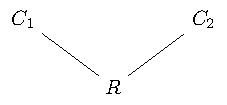
\includegraphics{resolvente-definicion.pdf}
    \end{center}

    \begin{ejemplo}\label{ej:resolvente-1}
        Sean $C_{1}=\{A_{1},\neg A_{2},A_{3}\}$ y $C_{2}=\{A_{2},\neg A_{3},A_{4}\}$. Dado que $A_{3}\in C_{1}$ y
        $\neg A_{3}\in C_{2}$, podemos hallar un resolvente.
        \begin{center}
            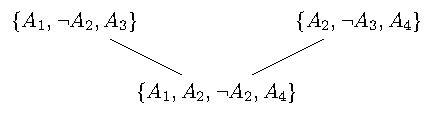
\includegraphics{resolvente-ejemplo1.pdf}
        \end{center}
    \end{ejemplo}

    \begin{ejemplo}\label{ej:resolvente-no-unico}
        El resolvente de dos cláusulas no es necesariamente único. En el ejemplo anterior, dado que $\neg A_{2}\in C_{1}$ y
        $A_{2}\in C_{2}$, también tenemos
        \begin{center}
            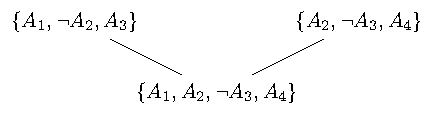
\includegraphics{resolvente-ejemplo2.pdf}
        \end{center}
    \end{ejemplo}

    Enumeramos ahora las tres reglas de deducción que se usan en la resolución.

    \begin{itemize}
        \item[$\bullet$] Sea $G$ cualquier fórmula. Sea $F$ la fórmula en FNC resultante de aplicar el Algoritmo FNC a $G$.
        Entonces $F$ puede deducirse de $G$.
        \item[$\bullet$] Sea $F$ una fórmula en FNC. Cualquier cláusula de $F$ puede deducirse de $F$.
        \item[$\bullet$] Sea $F$ una fórmula en FNC. Cualquier resolvente de dos cláusulas de $F$ puede deducirse de $F$.
    \end{itemize}

    Sorprendentemente, estas tres reglas bastan para la lógica proposicional. La resolución es completa. Antes de demostrar
    este hecho, debemos verificar que estas reglas son correctas. Mostramos algo más fuerte. Mostramos que cada una de estas
    reglas puede deducirse usando demostraciones formales. En la primera regla, $F$ puede deducirse de $G$ por la
    Proposición \ref{prop:fnc-fnd-demostrable}. Si $C$ es una cláusula de $F$, entonces podemos deducir $C$ a partir de $F$
    usando $\wedge$-Simetría y $\wedge$-Eliminación.\\
    Resta mostrar que $R$ puede deducirse de $F$ donde $R$ es un resolvente de dos cláusulas de $F$. Obsérvese la similitud
    entre esto y la regla del corte. Sean $C_{1}$ y $C_{2}$ como en el Ejemplo \ref{ej:resolvente-1}. Entonces $C_{1}$ es
    equivalente a $(\neg A_{1}\wedge A_{2})\rightarrow A_{3}$ y $C_{2}$ es equivalente a $A_{3}\rightarrow(A_{2}\vee A_{4})$.
    La regla del corte afirma que, a partir de estas fórmulas, podemos deducir la fórmula
    $(\neg A_{1}\wedge A_{2})\rightarrow(A_{2}\vee A_{4})$. Esta fórmula es equivalente al resolvente obtenido en el
    Ejemplo \ref{ej:resolvente-1}.

    \begin{proposicion}\label{prop:resolvente-deducible}
        Sean $C_{1}$ y $C_{2}$ cláusulas y sea $R$ un resolvente de $C_{1}$ y $C_{2}$. Entonces $\{C_{1},C_{2}\}\vdash R$.
    \end{proposicion}
    \begin{proof}
        Dado que $C_{1}$ y $C_{2}$ tienen un resolvente, debe existir una fórmula atómica $A$ tal que $A$ está en una de
        estas cláusulas y $\neg A$ está en la otra. Sin pérdida de generalidad, podemos suponer que $A$ está en $C_{1}$ y
        $\neg A$ está en $C_{2}$. Así, $C_{1}$ es equivalente a $(A\vee F)$ para alguna cláusula $F$ y $C_{2}$ es equivalente
        a $(\neg A\vee G)$ para alguna cláusula $G$. La fórmula $(F\vee G)$ es un resolvente de $C_{1}$ y $C_{2}$. Podemos
        suponer que $R$ es este resolvente. Damos una demostración formal de $\{C_{1},C_{2}\}\vdash R$.

        \begin{quote}
            Premisa: $\FF\vdash(A\vee F)$ y $\FF\vdash(\neg A\vee G)$\\
            Conclusión: $\FF\vdash(F\vee G)$
        \end{quote}

        \begin{derivacion}
            1. $\FF\vdash(A\vee F)$ & Premisa\\
            2. $\FF\cup\{\neg A\}\vdash(A\vee F)$ & Monotonicidad aplicada a 1\\
            3. $\FF\cup\{\neg A\}\vdash\neg A$ & Suposición\\
            4. $\FF\cup\{\neg A\}\vdash F$ & $\vee$-Eliminación aplicada a 2 y 3\\
            5. $\FF\cup\{\neg A\}\vdash(F\vee G)$ & $\vee$-Introducción aplicada a 4\\
            6. $\FF\vdash(\neg A\vee G)$ & Premisa\\
            7. $\FF\cup\{\neg\neg A\}\vdash(\neg A\vee G)$ & Monotonicidad aplicada a 1\\
            8. $\FF\cup\{\neg\neg A\}\vdash\neg\neg A$ & Suposición\\
            9. $\FF\cup\{\neg\neg A\}\vdash G$ & $\vee$-Eliminación aplicada a 7 y 8\\
            10. $\FF\cup\{\neg\neg A\}\vdash(G\vee F)$ & $\vee$-Introducción aplicada a 9\\
            11. $\FF\cup\{\neg\neg A\}\vdash(F\vee G)$ & $\vee$-Simetría aplicada a 10\\
            12. $\FF\vdash(F\vee G)$ & Demostración por casos aplicada a 5 y 11\\
        \end{derivacion}
    \end{proof}

    Así, cualquier cosa que pueda demostrarse usando resolución puede recibir una demostración formal. Se sigue entonces del
    Teorema \ref{thm:correccion} que la resolución es correcta. En particular, si $R$ es el resolvente de dos cláusulas de
    una fórmula $F$ en FNC, entonces $R$ es consecuencia de $F$. Aparentemente, la resolución es un fragmento de nuestro
    sistema de demostración formal. Como mostramos ahora, la resolución es tan poderosa como las demostraciones formales.

    \subsection{Completitud de la resolución}

    Mostramos que la resolución puede usarse para determinar si una fórmula dada es satisfacible o no. Podemos suponer que
    la fórmula está en FNC. Dada cualquier fórmula $F$ en FNC, sea $\mathrm{Res}_{0}(F)=\{C\mid C\text{ es una cláusula de }F\}$.
    Para cada $n>0$, sea
    \begin{equation*}
        \mathrm{Res}_{n}(F)=\mathrm{Res}_{n-1}(F)\cup\{R\mid R\text{ es un resolvente de dos cláusulas de }\mathrm{Res}_{n-1}(F)\}.
    \end{equation*}
    Dado que $\mathrm{Res}_{0}(F)=F$ es un conjunto finito, solo hay finitas cláusulas que pueden deducirse de $F$ usando
    resolventes. De hecho, solo hay finitas cláusulas que usan las mismas fórmulas atómicas que $F$. Así, eventualmente
    hallaremos algún $m$ tal que $\mathrm{Res}_{m}(F)=\mathrm{Res}_{m+1}(F)$. Sea $\mathrm{Res}^{*}(F)$ este $\mathrm{Res}_{m}(F)$.
    Este es el conjunto de todas las cláusulas que pueden deducirse de $F$ usando resolventes. Viéndolo como una fórmula,
    $\mathrm{Res}^{*}(F)$ es la conjunción de todas las consecuencias de $F$ que pueden deducirse mediante resolventes.

    \begin{proposicion}\label{prop:vacio-implica-insatisfacible}
        Sea $F$ una fórmula en FNC. Si $\emptyset\in\mathrm{Res}^{*}(F)$, entonces $F$ es insatisfacible.
    \end{proposicion}
    \begin{proof}
        Si $\emptyset\in\mathrm{Res}^{*}(F)$, entonces $\emptyset\in\mathrm{Res}_{n}(F)$ para algún $n$. Dado que
        $\emptyset\notin\mathrm{Res}_{0}(F)$ ($\emptyset$ no es una cláusula), debe existir algún $m$ tal que
        $\emptyset\notin\mathrm{Res}_{m}(F)$ y $\emptyset\in\mathrm{Res}_{m+1}(F)$, en cuyo caso $\emptyset$ es el resolvente
        de dos cláusulas de $\mathrm{Res}_{m}(F)$. Pero $\emptyset$ solo puede obtenerse como el resolvente de $\{A\}$ y
        $\{\neg A\}$ para alguna $A$ atómica. Tanto $\{A\}$ como $\{\neg A\}$ deben estar en $\mathrm{Res}_{m}(F)$. Por la
        proposición anterior, tanto $A$ como $\neg A$ son consecuencias de $F$. Se sigue que $A\wedge\neg A$ es consecuencia
        de $F$ y $F$ es insatisfacible.
    \end{proof}

    \begin{ejemplo}\label{ej:resolucion-insatisfacible}
        Sea $F$ la fórmula
        \begin{equation*}
            \{\{A,B,\neg C\},\{\neg A\},\{A,B,C\},\{A,\neg B\}\}.
        \end{equation*}
        Mostramos que $F$ es insatisfacible usando resolución.\\
        Sean $C_{1}$, $C_{2}$, $C_{3}$ y $C_{4}$ las cuatro cláusulas de $F$ en el orden dado anteriormente.
        \begin{center}
            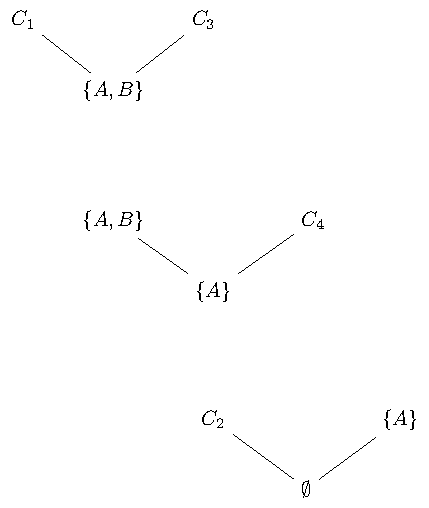
\includegraphics{resolucion-cadena.pdf}
        \end{center}

        Vemos que $\{A,B\}\in\mathrm{Res}(F)$, $\{A\}\in\mathrm{Res}_{2}(F)$, y $\emptyset\in\mathrm{Res}_{3}(F)$. Por la
        Proposición \ref{prop:vacio-implica-insatisfacible}, $F$ es insatisfacible. Podemos organizar esto como una
        demostración de dos columnas de la siguiente manera.

        \begin{center}
        \renewcommand{\arraystretch}{1.35}
        \begin{tabular}{@{}l l@{}}
            \textbf{Consecuencia de $F$} & \textbf{Justificación}\\
            \hline
            $C_{1}$ & Cláusula de $F$\\
            $C_{3}$ & Cláusula de $F$\\
            $\{A,B\}$ & Resolvente de $C_{1}$ y $C_{2}$\\
            $C_{4}$ & Cláusula de $F$\\
            $\{A\}$ & Resolvente de $\{A,B\}$ y $C_{4}$\\
            $C_{2}$ & Cláusula de $F$\\
            $\emptyset$ & Resolvente de $\{A\}$ y $C_{2}$\\
        \end{tabular}
        \end{center}
    \end{ejemplo}

    Consideremos ahora el recíproco de la Proposición \ref{prop:vacio-implica-insatisfacible}. Sea $F$ una fórmula en FNC.
    Si $F$ es insatisfacible, ¿debe entonces $\emptyset$ estar en $\mathrm{Res}^{*}(F)$? Mostramos que la respuesta es
    \comillas{sí.} La resolución es todo lo que necesitamos para mostrar insatisfacibilidad. Esto no es evidente de
    inmediato. Después de todo, para la columna de \comillas{Justificación} de estas demostraciones, solo tenemos dos
    opciones. O bien se da una cláusula, o bien es un resolvente de dos cláusulas deducidas previamente. Podría parecer que
    este método de demostración es demasiado restrictivo. Demostramos que no lo es.

    \begin{proposicion}\label{prop:insatisfacible-implica-vacio}
        Sea $F$ una fórmula en FNC. Si $F$ es insatisfacible, entonces $\emptyset\in\mathrm{Res}^{*}(F)$.
    \end{proposicion}
    \begin{proof}
        Sea $F=\{C_{1},\dots,C_{k}\}$. Suponemos que ninguna de las $C_{i}$ es una tautología (en caso contrario,
        simplemente descartamos estas cláusulas y mostramos que $\emptyset$ puede deducirse de lo que resta). Demostraremos
        esta proposición por inducción sobre el número $n$ de fórmulas atómicas que ocurren en $F$.\\
        Sea $n=1$. Sea $A$ la única fórmula atómica que ocurre en $F$. Entonces solo hay tres cláusulas posibles en $F$. Cada
        $C_{i}$ es $\{A\}$, $\{\neg A\}$, o $\{A,\neg A\}$. La última cláusula es una tautología y, por nuestra suposición
        anterior, no es una cláusula de $F$. Así, las únicas cláusulas en $F$ son $\{A\}$ y $\{\neg A\}$. Hay tres
        posibilidades: $F=\{\{A\}\}$, $F=\{\{\neg A\}\}$, o $F=\{\{A\},\{\neg A\}\}$. Las dos primeras son satisfacibles. Así,
        $F$ debe ser $\{\{A\},\{\neg A\}\}$. Claramente, $\emptyset\in\mathrm{Res}^{*}(F)$.\\
        Supongamos ahora que $F$ tiene subfórmulas atómicas $A_{1},\dots,A_{n+1}$. Supongamos además que
        $\emptyset\in\mathrm{Res}^{*}(G)$ para cualquier fórmula insatisfacible $G$ que use únicamente las fórmulas atómicas
        $A_{1},\dots,A_{n}$.\\
        Definimos algunas fórmulas nuevas. Sea $\widetilde{F}_{0}$ la conjunción de todas las $C_{i}$ de $F$ que no
        contienen a $\neg A_{n+1}$. Sea $\widetilde{F}_{1}$ la conjunción de todas las $C_{i}$ de $F$ que no contienen a
        $A_{n+1}$. Estas son fórmulas en FNC. Afirmamos que, al verlas como conjuntos,
        \begin{equation*}
            \widetilde{F}_{0}\cup\widetilde{F}_{1}=F.
        \end{equation*}
        Pues, supongamos que hay alguna cláusula $C_{i}$ de $F$ que no está en $\widetilde{F}_{0}\cup\widetilde{F}_{1}$.
        Entonces $C_{i}$ debe contener tanto a $A_{n+1}$ como a $\neg A_{n+1}$. Pero entonces $C_{i}$ es una tautología, lo
        cual contradice nuestra suposición anterior. Así, $\widetilde{F}_{0}\cup\widetilde{F}_{1}$ y $F$ contienen las mismas
        cláusulas.\\
        Sea $F_{0}=\{C_{i}-\{A_{n+1}\}\mid C_{i}\in\widetilde{F}_{0}\}$.\\
        Sea $F_{1}=\{C_{i}-\{\neg A_{n+1}\}\mid C_{i}\in\widetilde{F}_{1}\}$.\\
        Es decir, $F_{0}$ se forma eliminando $A_{n+1}$ de cada cláusula de $\widetilde{F}_{0}$ en la que aparece. De igual
        manera, $F_{1}$ se obtiene eliminando $\neg A_{n+1}$ de cada cláusula de $\widetilde{F}_{1}$.\\
        Afirmamos que, si reemplazamos $A_{n+1}$ en $F$ por una contradicción, entonces la fórmula resultante es equivalente
        a $F_{0}$. Y si reemplazamos $A_{n+1}$ en $F$ por una tautología, entonces la fórmula resultante es equivalente a
        $F_{1}$. Damos un ejemplo para ilustrar esto, pero dejamos al lector la verificación de este hecho.

        \begin{ejemplo}\label{ej:reduccion-atomicas}
            Supongamos que $n=2$, de modo que $A_{n+1}$ es $A_{3}$.\\
            Sea $F=\{\{A_{1},A_{3}\},\{A_{2}\},\{\neg A_{1},\neg A_{2},A_{3}\},\{\neg A_{2},\neg A_{3}\}\}$.\\
            Entonces $\widetilde{F}_{0}=\{\{A_{1},A_{3}\},\{A_{2}\},\{\neg A_{1},\neg A_{2},A_{3}\}\}$\\
            y $\widetilde{F}_{1}=\{\{A_{2}\},\{\neg A_{2},\neg A_{3}\}\}$.\\
            Así, $F_{0}=\{\{A_{1}\},\{A_{2}\},\{\neg A_{1},\neg A_{2}\}\}$\\
            y $F_{1}=\{\{A_{2}\},\{\neg A_{2}\}\}$.\\
            Ahora bien, $F$ es la fórmula $(A_{1}\vee A_{3})\wedge(A_{2})\wedge(\neg A_{1}\vee\neg A_{2}\vee A_{3})\wedge(\neg A_{2}\vee\neg A_{3})$.\\
            Si sabemos que $A_{3}$ tiene valor de verdad 0, esto se convierte en
            $(A_{1}\vee 0)\wedge(A_{2})\wedge(\neg A_{1}\vee\neg A_{2}\vee 0)\wedge(1)$, que es equivalente a $F_{0}$.\\
            Si sabemos que $A_{3}$ tiene valor de verdad 1, entonces $F$ se reduce a
            $(1)\wedge(A_{2})\wedge(1)\wedge(\neg A_{2}\vee 0)$, que es equivalente a $F_{1}$.
        \end{ejemplo}

        Dado que $A_{n+1}$ debe tener valor de verdad 0 o 1, se sigue que $F\equiv F_{0}\vee F_{1}$. Dado que $F$ es
        insatisfacible, $F_{0}$ y $F_{1}$ son cada una insatisfacible. Las fórmulas $F_{0}$ y $F_{1}$ solo usan las fórmulas
        atómicas $A_{1},\dots,A_{n}$. Por nuestra hipótesis de inducción, $\emptyset\in\mathrm{Res}^{*}(F_{0})$ y
        $\emptyset\in\mathrm{Res}^{*}(F_{1})$. (Obsérvese que $\emptyset$ puede deducirse fácilmente tanto de $F_{0}$ como de
        $F_{1}$ en nuestro ejemplo.)\\
        Ahora bien, $F_{0}$ se formó a partir de $\widetilde{F}_{0}$ eliminando $A_{n+1}$ de cada cláusula. Dado que podemos
        deducir $\emptyset$ a partir de $F_{0}$, podemos deducir $\emptyset$ o $\{A_{n+1}\}$ a partir de $\widetilde{F}_{0}$
        (reinstaurando $\{A_{n+1}\}$ en cada cláusula de $F_{0}$). De igual manera, podemos deducir $\emptyset$ o
        $\{\neg A_{n+1}\}$ a partir de $\widetilde{F}_{1}$. Si podemos deducir $\{A_{n+1}\}$ de $F_{0}$ y $\{\neg A_{n+1}\}$
        de $F_{1}$, entonces podemos deducir $\emptyset$ de $\widetilde{F}_{0}\cup\widetilde{F}_{1}$. Dado que
        $F=\widetilde{F}_{0}\cup\widetilde{F}_{1}$, concluimos que $\emptyset\in\mathrm{Res}^{*}(F)$.
    \end{proof}

    Esto proporciona un algoritmo para el problema de satisfacibilidad. Dada cualquier fórmula $G$, primero hallamos una
    fórmula $F$ en FNC que sea equivalente a $G$ (usando el Algoritmo FNC). Luego calculamos el conjunto finito
    $\mathrm{Res}^{*}(F)$. Si $\emptyset\in\mathrm{Res}^{*}(F)$, el algoritmo concluye \comillas{No, $G$ no es satisfacible.}
    En caso contrario, concluye \comillas{Sí, $G$ es satisfacible.} Por las Proposiciones
    \ref{prop:vacio-implica-insatisfacible} y \ref{prop:insatisfacible-implica-vacio}, este algoritmo funciona. Este
    algoritmo no es necesariamente rápido. Como mencionamos anteriormente, no se conoce ningún algoritmo de tiempo
    polinomial para este problema de decisión. Sin embargo, en ciertos casos, este algoritmo puede llegar rápidamente a una
    conclusión. Si $F$ es insatisfacible, no necesariamente tenemos que calcular todo $\mathrm{Res}^{*}(F)$. En cuanto
    aparece $\emptyset$, sabemos que no es satisfacible. Si $F$ es satisfacible, por otro lado, entonces las tablas de
    verdad pueden llegar rápidamente a una conclusión. Solo necesitamos calcular la tabla de verdad hasta hallar un valor de
    verdad de 1.\\
    Resumimos los principales resultados de esta sección en el siguiente teorema. Este teorema es una versión finita del
    Teorema de completitud para la lógica proposicional.

    \begin{teorema}\label{thm:completitud-finita}
        Sean $F$ y $G$ fórmulas de la lógica proposicional. Sea $H$ la fórmula en FNC obtenida al aplicar el Algoritmo FNC a
        la fórmula $F\wedge\neg G$. Las siguientes afirmaciones son equivalentes:
        \begin{enumerate}
            \item[1.] $F\models G$
            \item[2.] $\{F\}\vdash G$
            \item[3.] $\emptyset\in\mathrm{Res}^{*}(H)$
        \end{enumerate}
    \end{teorema}
    \begin{proof}
        (2) implica (1) por el Teorema \ref{thm:correccion}.\\
        (1) implica (3) por la Proposición \ref{prop:insatisfacible-implica-vacio}.\\
        Debemos mostrar que (3) implica (2). Por la Proposición \ref{prop:fnc-fnd-demostrable}, tenemos
        $\{F\wedge\neg G\}\vdash H$. Por $\wedge$-Introducción, $\{F,\neg G\}\vdash F\wedge\neg G$. Se sigue que
        $\{F,\neg G\}\vdash H$.\\
        Dado que $\emptyset\in\mathrm{Res}^{*}(H)$, debe existir una fórmula atómica $A$ tal que tanto $\{A\}$ como
        $\{\neg A\}$ están en $\mathrm{Res}^{*}(H)$. Se sigue de la Proposición \ref{prop:resolvente-deducible} que tanto
        $\{H\}\vdash A$ como $\{H\}\vdash\neg A$. Por lo tanto, tanto
        \begin{equation*}
            \{F,\neg G\}\vdash A\quad\text{como}\quad\{F,\neg G\}\vdash\neg A.
        \end{equation*}
        Por demostración por contradicción, tenemos $\{F\}\vdash\neg\neg G$. Finalmente, $\{F\}\vdash G$ por Doble negación.
    \end{proof}

    \section{Completitud y compacidad}

    La completitud y la compacidad son dos propiedades que una lógica puede o no poseer. Concluimos nuestro estudio de la
    lógica proposicional mostrando que esta lógica posee, en efecto, cada una de estas propiedades.\\
    Una lógica es un lenguaje formal que cuenta con reglas para deducir la verdad de un enunciado a partir de la de otro. Si
    una sentencia $G$ puede deducirse de un conjunto de sentencias $\FF$ usando estas reglas, entonces escribimos
    $\FF\vdash G$. La notación $\FF\models G$, por otro lado, significa que siempre que cada sentencia de $\FF$ sea
    verdadera, $G$ también lo es. Si $\FF\vdash G$, entonces $\FF\models G$. Lo contrario, sin embargo, no es
    necesariamente cierto. Dicho de otra manera, $\FF\models G$ significa que $\FF$ implica $G$ y $\FF\vdash G$ significa que
    podemos demostrar que $\FF$ implica $G$ usando las reglas de la lógica. Pero que algo sea verdadero no significa que
    podamos demostrarlo. Quizá las reglas de la lógica son demasiado débiles para demostrar todo (o el poder expresivo de la
    lógica es demasiado fuerte). Si podemos demostrar todo lo que es verdadero (es decir, si $\FF\models G$ sí implica
    $\FF\vdash G$), entonces decimos que la lógica es \textit{completa}.

    \begin{quote}
        (Completitud:) $\FF\models G$ si y solo si $\FF\vdash G$.
    \end{quote}

    En la Sección 1.4 definimos la notación $\FF\vdash G$ para la lógica proposicional enumerando un conjunto de reglas. Sin
    embargo, la completitud debe entenderse no como un enunciado sobre estas reglas específicas, sino como un enunciado
    sobre la lógica misma. La completitud afirma la existencia de una lista de reglas que nos permite deducir toda
    consecuencia a partir de cualquier conjunto de fórmulas de la lógica. Para demostrar esto necesitamos exhibir tal lista
    de reglas. Mostramos que las reglas de las Tablas 1.5 y 1.6, junto con las reglas de la resolución, bastan para la
    lógica proposicional. Como veremos en el Capítulo 9, la lógica de segundo orden no tiene completitud. No podemos dar una
    lista agradable de reglas que nos permita deducir toda consecuencia a partir de cualquier conjunto de sentencias de
    segundo orden.\\
    Para demostrar que la lógica proposicional tiene completitud, debemos pasar de conjuntos finitos a conjuntos infinitos
    de fórmulas. Si $F$ es finito, entonces $F\models G$ si y solo si $F\vdash G$ por el Teorema
    \ref{thm:completitud-finita}. Supongamos ahora que $F$ es infinito. Si $F$ es un conjunto de fórmulas en FNC, entonces
    puede verse como un conjunto de cláusulas. El conjunto $\mathrm{Res}_{n}(F)$ se define como se hizo para conjuntos
    finitos de cláusulas. Sea $\mathrm{Res}^{*}(F)$ la unión de todos los conjuntos $\mathrm{Res}_{n}(F)$ (para $n\in\N$). De
    nuevo, $\mathrm{Res}^{*}(F)$ es el conjunto de todas las cláusulas que pueden deducirse de $F$ usando resolución. Si $F$
    es infinito, entonces $\mathrm{Res}^{*}(F)$ es infinito y no puede verse como una fórmula. Tal conjunto infinito de
    cláusulas es satisfacible si y solo si existe una asignación que modela cada cláusula del conjunto. Para demostrar que
    la lógica proposicional tiene completitud, basta demostrar lo siguiente.

    \begin{proposicion}\label{prop:res-infinito}
        Sea $F$ un conjunto de fórmulas en FNC. Entonces $\emptyset\in\mathrm{Res}^{*}(F)$ si y solo si $F$ es
        insatisfacible.
    \end{proposicion}
    \begin{proof}
        Para $F$ finito, esto es una reformulación de las Proposiciones \ref{prop:vacio-implica-insatisfacible} y
        \ref{prop:insatisfacible-implica-vacio}. Recordemos las demostraciones de estos dos enunciados. Para la Proposición
        \ref{prop:insatisfacible-implica-vacio}, supusimos que $F$ era insatisfacible, y demostramos que
        $\emptyset\in\mathrm{Res}^{*}(F)$ por inducción sobre el número de fórmulas atómicas que ocurren en $F$. Pero la
        inducción matemática solo demuestra que algo es verdadero para todo $n$ finito. Así, el método que usamos para
        demostrar la Proposición \ref{prop:insatisfacible-implica-vacio} no funciona si $F$ involucra infinitas fórmulas
        atómicas.\\
        Consideremos la otra dirección de la Proposición \ref{prop:res-infinito}. Supongamos que
        $\emptyset\in\mathrm{Res}^{*}(F)$. Entonces $\emptyset\in\mathrm{Res}_{n}(F)$ para algún $n$. Es decir, podemos
        deducir $\emptyset$ a partir de $F$ en un número finito de pasos. Por lo tanto, podemos deducir $\emptyset$ a partir
        de algún subconjunto finito $F'$ de $F$. Por la Proposición \ref{prop:vacio-implica-insatisfacible}, $F'$ es
        insatisfacible. Dado que $F'$ es un subconjunto de $F$, $F$ también debe ser insatisfacible.\\
        Así, una dirección de la Proposición \ref{prop:res-infinito} se sigue de los resultados de la sección anterior.
        Podemos deducir el caso infinito a partir del caso finito observando que, si $\emptyset$ puede deducirse de $F$,
        entonces puede deducirse de algún subconjunto finito de $F$. Para demostrar la otra dirección de la Proposición
        \ref{prop:res-infinito} necesitamos una idea análoga. Necesitamos mostrar que si $F$ es insatisfacible, entonces
        algún subconjunto finito de $F$ es insatisfacible. Esto se conoce como \textit{compacidad}. Completamos esta
        demostración más adelante en esta sección, una vez establecida la compacidad de la lógica proposicional (Teorema
        \ref{thm:compacidad}).
    \end{proof}

    \begin{quote}
        \textbf{Compacidad:} $F$ es insatisfacible si y solo si algún subconjunto finito de $F$ es insatisfacible.
    \end{quote}

    Dicho de otra manera, la compacidad afirma que $F$ es satisfacible si y solo si todo subconjunto finito de $F$ es
    satisfacible. Al igual que con la completitud, una dirección de la compacidad siempre se cumple. Si $F$ es satisfacible,
    entonces todo subconjunto finito de $F$ también debe ser satisfacible. Pero el hecho de que todo subconjunto finito de
    un conjunto sea satisfacible no significa necesariamente que el conjunto mismo lo sea. Consideremos, por ejemplo, el
    siguiente conjunto de oraciones en español.

    \begin{quote}
        $F_{0}=$ \comillas{Hay finitos objetos en el universo.}\\
        $F_{1}=$ \comillas{Hay al menos un objeto en el universo.}\\
        $F_{2}=$ \comillas{Hay al menos dos objetos en el universo.}\\
        $F_{3}=$ \comillas{Hay al menos tres objetos en el universo.}\\
        $\dots$\\
        $F_{n}=$ \comillas{Hay al menos $n$ objetos en el universo.}\\
        $\dots$
    \end{quote}

    Tomadas en conjunto, estas oraciones son contradictorias. Si hay más de $n$ objetos para cada $n$, entonces no puede
    haber finitos objetos, como afirma $F_{0}$. Sin embargo, si tomamos solo finitas de las afirmaciones anteriores, no hay
    ningún problema. Cualquier conjunto finito de estas oraciones es satisfacible, pero la colección completa no lo es.
    Cualquier lógica que pueda expresar estas oraciones no tiene compacidad.\\
    Demostramos que la lógica proposicional sí tiene compacidad en el Teorema \ref{thm:compacidad}. Primero, demostramos el
    siguiente lema. Este lema puede no parecer relevante por el momento, pero es la clave para demostrar el Teorema
    \ref{thm:compacidad}.

    \begin{lema}\label{lema:cadenas-binarias}
        Sea $X$ un conjunto infinito de cadenas binarias finitas. Existe una cadena binaria infinita $\bar{w}$ tal que
        cualquier prefijo de $\bar{w}$ es también prefijo de infinitas $\bar{x}$ en $X$.
    \end{lema}
    \begin{proof}
        Una cadena binaria es una sucesión de ceros y unos, como $1011$. Las cadenas $1$, $10$, $101$ y $1011$ son los
        prefijos de $1011$. Tenemos un conjunto infinito $X$ de tales cadenas de longitud finita. Queremos construir una
        cadena infinita $\bar{w}$ de ceros y unos tal que cada prefijo de $\bar{w}$ sea también prefijo de infinitas
        cadenas de $X$.\\
        Construimos $\bar{w}$ paso a paso, de izquierda a derecha. En cada paso haremos dos cosas. En el paso $n$-ésimo, no
        solo decidimos cuál debe ser el $n$-ésimo dígito de $\bar{w}$, sino que también eliminamos de $X$ las cadenas que no
        nos convienen.\\
        Para determinar cuál debe ser el primer dígito de $\bar{w}$, observamos los primeros dígitos de todas las cadenas de
        $X$. Por supuesto, hay infinitas cadenas y no podemos observar todos estos dígitos a la vez, pero supongamos que
        somos, de alguna manera, omniscientes. Hay dos posibilidades. O bien vemos infinitos unos, o no los vemos. Si
        infinitas cadenas de $X$ comienzan con 1, entonces hacemos que el primer dígito de $\bar{w}$ sea 1 y eliminamos
        todas las cadenas de $X$ que comienzan con 0 (todavía nos quedan infinitas). En caso contrario, si solo finitas
        cadenas de $X$ comienzan con 1, las eliminamos y hacemos que el primer dígito de $\bar{w}$ sea 0.\\
        Supongamos ahora que hemos determinado los primeros $n$ dígitos de $\bar{w}$. Supongamos también que hemos
        eliminado de $X$ todas las sucesiones que no comienzan con estos mismos $n$ dígitos y que nos queda un subconjunto
        infinito $X'$ de $X$. Para determinar la entrada $(n+1)$-ésima de $\bar{w}$ observamos los dígitos $(n+1)$-ésimos de
        todas las cadenas de $X'$. Dado que $X'$ es infinito, $X'$ debe tener infinitas cadenas de longitud $n+1$ o mayor.
        Así, de nuevo hay dos posibilidades. Si infinitas cadenas de $X'$ tienen un 1 en la posición $(n+1)$-ésima, entonces
        hacemos que el dígito $(n+1)$-ésimo de $\bar{w}$ sea 1. En caso contrario, hacemos que el dígito $(n+1)$-ésimo sea 0.
        En cualquier caso, eliminamos todas las cadenas de $X'$ que no comparten las mismas primeras $n+1$ entradas que
        $\bar{w}$. Todavía nos queda un subconjunto infinito de $X$.\\
        Continuando este procedimiento, obtenemos una sucesión infinita $\bar{w}$ tal que los primeros $n$ dígitos de
        $\bar{w}$ coinciden con los primeros $n$ dígitos de infinitas sucesiones de $X$. En realidad no hemos dado una
        manera práctica de construir $\bar{w}$, pero hemos demostrado que tal cadena existe.
    \end{proof}

    Estamos listos ahora para demostrar que la lógica proposicional tiene compacidad.

    \begin{teorema}[Compacidad de la lógica proposicional]\label{thm:compacidad}
        Un conjunto de sentencias de la lógica proposicional es satisfacible si y solo si todo subconjunto finito es
        satisfacible.
    \end{teorema}
    \begin{proof}
        Como señalamos anteriormente, solo una dirección de esto requiere demostración. Supongamos que
        $F=\{F_{1},F_{2},\dots\}$ es un conjunto de fórmulas y que todo subconjunto finito de $F$ es satisfacible. Sean
        $A_{1},A_{2},A_{3},\dots$ una lista sin repetición de las fórmulas atómicas que ocurren en $F_{1}$, seguidas de las
        fórmulas atómicas que ocurren en $F_{2}$ (pero no en $F_{1}$), y así sucesivamente.\\
        Dado que todo subconjunto finito de $F$ es satisfacible, para cada $n$ existe una asignación $\AA_{n}$ tal que
        $\AA_{n}\models\bigwedge_{i=1}^{n}F_{i}$. Así, cada $F_{i}$ de $F$ se cumple bajo todas, salvo a lo sumo finitas, de
        estas asignaciones. Podemos suponer que $\AA_{n}$ está definida únicamente sobre las fórmulas atómicas que ocurren
        en $F_{1},\dots,F_{n}$. Para cada $n$, los valores de verdad que $\AA_{n}$ asigna a $A_{1},A_{2},\dots$ forman una
        sucesión finita de ceros y unos. Así, $X=\{\AA_{n}\mid n=1,2,\dots\}$ es un conjunto infinito de sucesiones binarias
        finitas. Por el lema anterior, existe una sucesión binaria infinita $\bar{w}$ tal que todo prefijo de $\bar{w}$ es
        prefijo de infinitas sucesiones de $X$.\\
        Definimos una asignación $\AA$ sobre todas las $\AA_{n}$ de la siguiente manera: sea $\AA(A_{n})$ el $n$-ésimo
        dígito de $\bar{w}$. Debemos mostrar que toda fórmula $F$ de $F$ se cumple bajo $\AA$. Esto se sigue del hecho de
        que $F$ se cumple bajo todas, salvo a lo sumo finitas, de las asignaciones de $X$. Sea $m$ tal que $F$ no contiene
        ninguna fórmula atómica posterior a $A_{m}$ en nuestra lista. Entonces existe una $\AA_{n}$ en $X$ tal que
        $\AA_{n}\models F$ y las primeras $m$ entradas de $\AA_{n}$ son las mismas que las de $\AA$. Se sigue que $\AA$
        también modela $F$.
    \end{proof}

    La Proposición \ref{prop:res-infinito} se sigue de la compacidad. Ahora podemos demostrar que la lógica proposicional
    tiene completitud. Podríamos dar una demostración similar a la del Teorema \ref{thm:completitud-finita} usando la
    Proposición \ref{prop:res-infinito} en lugar de las Proposiciones \ref{prop:vacio-implica-insatisfacible} y
    \ref{prop:insatisfacible-implica-vacio}. Sin embargo, la compacidad produce una demostración más directa.

    \begin{teorema}[Completitud de la lógica proposicional]\label{thm:completitud}
        Para cualquier sentencia $G$ y conjunto de sentencias $\FF$, $\FF\models G$ si y solo si $\FF\vdash G$.
    \end{teorema}
    \begin{proof}
        Por el Teorema \ref{thm:correccion}, si $\FF\vdash G$, entonces $\FF\models G$.\\
        Recíprocamente, supongamos que $\FF\models G$. Entonces $\FF\cup\{\neg G\}$ es insatisfacible. Por compacidad,
        algún subconjunto finito de $\FF\cup\{\neg G\}$ es insatisfacible. Así, existe un $\FF_{0}\subset\FF$ finito tal
        que $\FF_{0}\cup\{\neg G\}$ es insatisfacible y, equivalentemente, $\FF_{0}\models G$. Dado que $\FF_{0}$ es finito,
        podemos aplicar el Teorema \ref{thm:completitud-finita} para obtener $\FF_{0}\vdash G$. Finalmente,
        $\FF\vdash G$ por Monotonicidad.
    \end{proof}

    \section*{Ejercicios}

    \begin{ejercicio}
        Muestre que $\neg$ y $\vee$ pueden tomarse como símbolos primitivos en la lógica proposicional. Es decir, muestre
        que cada uno de los símbolos $\wedge$, $\rightarrow$ y $\ssi$ puede definirse en términos de $\neg$ y $\vee$.
    \end{ejercicio}

    \begin{ejercicio}
        Muestre que $\neg$ y $\rightarrow$ pueden tomarse como símbolos primitivos en la lógica proposicional. Es decir,
        muestre que cada uno de los símbolos $\wedge$, $\vee$ y $\ssi$ puede definirse en términos de $\neg$ y $\rightarrow$.
    \end{ejercicio}

    \begin{ejercicio}\label{ej:tablas-verdad-varias}
        Halle las tablas de verdad para cada una de las siguientes fórmulas. Indique si cada una es una tautología, una
        contradicción, o ninguna de las dos.
        \begin{enumerate}[label=(\alph*)]
            \item $(\neg A\rightarrow B)\vee((A\wedge\neg C)\ssi B)$
            \item $(A\rightarrow B)\wedge(A\rightarrow\neg B)$
            \item $(A\rightarrow(B\vee C))\vee(C\rightarrow\neg A)$
            \item $((A\rightarrow B)\wedge C)\vee(A\wedge D)$
        \end{enumerate}
    \end{ejercicio}

    \begin{ejercicio}
        En cada uno de los siguientes casos, determine si las dos fórmulas son equivalentes.
        \begin{enumerate}[label=(\alph*)]
            \item $(A\wedge B)\vee C$ y $(A\rightarrow\neg B)\rightarrow C$
            \item $(((A\rightarrow B)\rightarrow B)\rightarrow B)$ y $(A\rightarrow B)$
            \item $(((A\rightarrow B)\rightarrow A)\rightarrow A)$ y $(C\rightarrow D)\vee C$
            \item $A\ssi((\neg A\wedge B)\vee(A\wedge\neg B))$ y $\neg B$
        \end{enumerate}
    \end{ejercicio}

    \begin{ejercicio}
        Muestre que los siguientes enunciados son equivalentes.
        \begin{enumerate}
            \item[1.] $F\models G$,
            \item[2.] $\models F\rightarrow G$,
            \item[3.] $F\wedge\neg G$ es insatisfacible, y
            \item[4.] $F\equiv F\wedge G$.
        \end{enumerate}
    \end{ejercicio}

    \begin{ejercicio}
        Muestre que los siguientes enunciados son equivalentes.
        \begin{enumerate}
            \item[1.] $F\equiv G$,
            \item[2.] $\models F\ssi G$, y
            \item[3.] $(F\wedge\neg G)\vee(\neg F\wedge G)$ es insatisfacible.
        \end{enumerate}
    \end{ejercicio}

    \begin{ejercicio}
        \begin{enumerate}[label=(\alph*)]
            \item Halle una fórmula $F$ en FNC que tenga la siguiente tabla de verdad.
            \begin{center}
            \renewcommand{\arraystretch}{1.4}
            \begin{tabular}{c | c | c | c}
                $A$ & $B$ & $C$ & $F$\\
                \hline
                0 & 0 & 0 & 0\\
                1 & 0 & 0 & 1\\
                0 & 1 & 0 & 1\\
                0 & 0 & 1 & 1\\
                1 & 1 & 0 & 0\\
                1 & 0 & 1 & 0\\
                0 & 1 & 1 & 0\\
                1 & 1 & 1 & 1\\
            \end{tabular}
            \end{center}
            \item Halle una fórmula en FND que tenga la tabla de verdad anterior.
        \end{enumerate}
    \end{ejercicio}

    \begin{ejercicio}
        Halle fórmulas en FNC equivalentes a cada una de las siguientes.
        \begin{enumerate}[label=(\alph*)]
            \item $(A\ssi B)\ssi C$
            \item $(A\rightarrow(B\vee C))\vee(C\rightarrow\neg A)$
            \item $(\neg A\wedge\neg B\wedge C)\vee(\neg A\wedge\neg C)\vee(B\wedge C)\vee A$.
        \end{enumerate}
    \end{ejercicio}

    \begin{ejercicio}
        La \textit{regla del corte} afirma que, a partir de las fórmulas $(F\rightarrow G)$ y $(G\rightarrow H)$, podemos
        deducir la fórmula $(F\rightarrow H)$. Verifique esta regla dando una demostración formal.
    \end{ejercicio}

    \begin{ejercicio}
        \begin{enumerate}[label=(\alph*)]
            \item Sea $\ssi$-Simetría la siguiente regla:
            \begin{quote}
                Premisa: $\FF\vdash(F\ssi G)$\\
                Conclusión: $\FF\vdash(G\ssi F)$
            \end{quote}
            Verifique esta regla dando una demostración formal.
            \item Dé una demostración formal de que $\{(F\ssi G)\}\vdash(\neg F\ssi\neg G)$.
        \end{enumerate}
    \end{ejercicio}

    \begin{ejercicio}
        Dé demostraciones formales de que las fórmulas $(F\wedge(F\vee G))$ y $(F\vee(F\wedge G))$ son equivalentes de
        manera demostrable.
    \end{ejercicio}

    \begin{ejercicio}
        Si $F\rightarrow G$ es consecuencia de $F$, entonces también lo es $\neg G\rightarrow\neg F$. Nos referimos a esta
        regla como $\rightarrow$-Contrapositiva. Verifique esta regla dando una demostración formal.
    \end{ejercicio}

    \begin{ejercicio}
        Muestre que $\vee$-Simetría se sigue de las demás reglas de las Tablas 1.5 y 1.6.
    \end{ejercicio}

    \begin{ejercicio}
        Muestre que $\rightarrow$-Eliminación se sigue de las demás reglas de las Tablas 1.5 y 1.6.
    \end{ejercicio}

    \begin{ejercicio}
        Muestre que Doble negación se sigue de Suposición, Monotonicidad y Demostración por casos.
    \end{ejercicio}

    \begin{ejercicio}
        Supongamos que eliminamos de la Tabla 1.5 las siguientes cuatro reglas: $\vee$-Eliminación, $\vee$-Simetría,
        $\rightarrow$-Introducción y $\rightarrow$-Eliminación, y las reemplazamos por las Leyes de De Morgan, la
        Distributividad de $\vee$, la regla del corte (Ejercicio 1.9), y el recíproco de Doble negación (si
        $\FF\vdash\neg\neg F$ entonces $\FF\vdash F$). Muestre que el conjunto de reglas resultante es completo.
    \end{ejercicio}

    \begin{ejercicio}
        Use resolución para verificar cada uno de los siguientes enunciados:
        \begin{enumerate}[label=(\alph*)]
            \item $\neg A$ es consecuencia de $(A\rightarrow B)\wedge(A\rightarrow\neg B)$
            \item $(\neg A\wedge\neg B\wedge C)\vee(\neg A\wedge\neg C)\vee(B\wedge C)\vee A$ es una tautología
            \item $((A\rightarrow B)\wedge(A\rightarrow\neg B))\rightarrow\neg A$ es una tautología.
        \end{enumerate}
    \end{ejercicio}

    \begin{ejercicio}
        Para cada fórmula del Ejercicio \ref{ej:tablas-verdad-varias}, halle una fórmula equivalente en FNC.
    \end{ejercicio}

    \begin{ejercicio}
        Para cada fórmula del Ejercicio \ref{ej:tablas-verdad-varias}, verifique su respuesta a ese problema usando
        resolución.
    \end{ejercicio}

    \begin{ejercicio}
        Determine si las siguientes fórmulas de Horn son satisfacibles o no. Si es satisfacible, halle una asignación que
        modele la fórmula.
        \begin{enumerate}[label=(\alph*)]
            \item $(T\rightarrow A_{1})\wedge(T\rightarrow A_{2})\wedge(A_{1}\wedge A_{2}\wedge A_{3}\rightarrow A_{4})
            \wedge(A_{1}\wedge A_{2}\wedge A_{4}\rightarrow A_{5})\wedge(A_{1}\wedge A_{2}\wedge A_{3}\wedge A_{4}\rightarrow A_{6})$\\
            $\wedge(A_{5}\wedge A_{6}\rightarrow A_{7})\wedge(A_{2}\rightarrow A_{3})\wedge(A_{7}\rightarrow\perp)$
            \item $(T\rightarrow A_{1})\wedge(T\rightarrow A_{2})\wedge(A_{1}\wedge A_{2}\wedge A_{4}\rightarrow A_{3})
            \wedge(A_{1}\wedge A_{5}\wedge A_{6})\wedge(A_{2}\wedge A_{7}\rightarrow A_{5})$\\
            $\wedge(A_{1}\wedge A_{3}\wedge A_{5}\rightarrow A_{7})\wedge(A_{2}\rightarrow A_{4})\wedge(A_{4}\rightarrow A_{8})
            \wedge(A_{2}\wedge A_{3}\wedge A_{4}\rightarrow A_{9})$\\
            $\wedge(A_{3}\wedge A_{9}\rightarrow A_{6})\wedge(A_{6}\wedge A_{7}\rightarrow A_{8})\wedge(A_{7}\wedge A_{8}\wedge A_{9}\rightarrow\perp)$
        \end{enumerate}
    \end{ejercicio}

    \begin{ejercicio}
        Considere la siguiente fórmula en FND.
        \begin{equation*}
            (A_{1}\wedge B_{1})\vee(A_{2}\wedge B_{2})\vee\dots\vee(A_{n}\wedge B_{n})
        \end{equation*}
        Dada esta fórmula como entrada, ¿cuántos pasos le tomará al Algoritmo FNC detenerse y producir una fórmula en FNC?
        ¿Es este algoritmo de tiempo polinomial?
    \end{ejercicio}

    \begin{ejercicio}\label{ej:completar-correccion}
        Complete la demostración del Teorema \ref{thm:correccion}.
    \end{ejercicio}

    \begin{ejercicio}\label{ej:completar-demorgan}
        Complete la demostración de la Proposición \ref{prop:demorgan-demostrable}.
    \end{ejercicio}

    \begin{ejercicio}\label{ej:distributividad-and-completa}
        Demuestre la Proposición \ref{prop:distributividad-and-demostrable} dando dos demostraciones formales.
    \end{ejercicio}

    \begin{ejercicio}\label{ej:distributividad-or-completa}
        Demuestre la Proposición \ref{prop:distributividad-or-demostrable}.
    \end{ejercicio}

    \begin{ejercicio}
        ¿Qué tiene de incorrecto la siguiente afirmación? ¿Por qué la \comillas{demostración falsa} dada no es una
        demostración?
        \begin{quote}
            \textbf{Afirmación:} $(A\rightarrow B)\vee C$ no es subfórmula de ninguna fórmula.\\[0.2cm]
            \textbf{Demostración [Falsa]} Sea $F$ cualquier fórmula. Mostramos que $(A\rightarrow B)\vee C$ no es
            subfórmula de $F$ por inducción sobre la complejidad de $F$.\\
            Si $F$ es atómica, entonces claramente $(A\rightarrow B)\vee C$ no es una subfórmula.\\
            Sean $F_{1}$ y $F_{2}$ dos fórmulas. Nuestra hipótesis de inducción es que ni $F_{1}$ ni $F_{2}$ tienen a
            $(A\rightarrow B)\vee C$ como subfórmula.\\
            Supongamos que $F$ es $\neg F_{1}$. Si $(A\rightarrow B)\vee C$ es subfórmula de $F$, entonces
            $(A\rightarrow B)\vee C$ es subfórmula de $F_{1}$ o es $F$ misma. No es subfórmula de $F_{1}$ por nuestra
            hipótesis de inducción. Además, dado que $(A\rightarrow B)\vee C$ no contiene el símbolo $\neg$, no puede ser
            $F$.\\
            Supongamos que $F$ es $F_{1}\wedge F_{2}$. Si $(A\rightarrow B)\vee C$ es subfórmula de $F$, entonces, dado que
            $(A\rightarrow B)\vee C$ no contiene el símbolo $\wedge$, debe ser subfórmula de $F_{1}$ o de $F_{2}$. Pero, por
            nuestra hipótesis de inducción, este no es el caso.\\
            Se sigue que $(A\rightarrow B)\vee C$ no es subfórmula de ninguna fórmula.
        \end{quote}
    \end{ejercicio}

    \begin{ejercicio}\label{ej:prop-distributividad-generalizada}
        Demuestre la Proposición \ref{prop:distributividad-generalizada} por inducción matemática. Es decir, dadas las
        fórmulas $\{F_{1},\dots,F_{n}\}$ y $\{G_{1},\dots,G_{m}\}$, demuestre cada uno de los siguientes enunciados por
        inducción sobre $n$.
        \begin{enumerate}[label=(\alph*)]
            \item $\left(\bigvee_{i=1}^{n}F_{i}\right)\vee\left(\bigvee_{j=1}^{m}G_{j}\right)\equiv
            \bigvee_{i=1}^{n}\bigvee_{j=1}^{m}(F_{i}\vee G_{j})$
            \item $\left(\bigwedge_{i=1}^{n}F_{i}\right)\wedge\left(\bigwedge_{j=1}^{m}G_{j}\right)\equiv
            \bigwedge_{i=1}^{n}\bigwedge_{j=1}^{m}(F_{i}\wedge G_{j})$.
        \end{enumerate}
    \end{ejercicio}

    \begin{ejercicio}\label{ej:sustitucion-demostrable-completa}
        Demuestre el Teorema \ref{thm:sustitucion-demostrable} por inducción sobre la complejidad de $H$.
    \end{ejercicio}

    \begin{ejercicio}
        Sean $\FF$ y $\GG$ conjuntos de fórmulas. Decimos que $\FF$ es equivalente a $\GG$, denotado $\FF\equiv\GG$, si para
        toda asignación $\AA$, $\AA\models\FF$ si y solo si $\AA\models\GG$.
        \begin{enumerate}[label=(\alph*)]
            \item Muestre que lo siguiente es verdadero:
            \begin{quote}
                Para cualesquiera $\FF$ y $\GG$, $\FF\equiv\GG$ si y solo si tanto\\
                $\FF\vdash G$ para cada $G\in\GG$ como\\
                $\GG\vdash F$ para cada $F\in\FF$.
            \end{quote}
            \item Demuestre que lo siguiente no es verdadero:
            \begin{quote}
                Para cualesquiera $\FF$ y $\GG$, $\FF\equiv\GG$ si y solo si tanto\\
                para cada $G\in\GG$ existe $F\in\FF$ tal que $G\models F$, como\\
                para cada $F\in\FF$ existe $G\in\GG$ tal que $F\models G$.
            \end{quote}
        \end{enumerate}
    \end{ejercicio}

    \begin{ejercicio}\label{ej:consistencia}
        Si una contradicción puede deducirse de un conjunto de sentencias, entonces se dice que el conjunto de sentencias
        es \textit{inconsistente}. En caso contrario, el conjunto de sentencias es \textit{consistente}. Sea $\FF$ un
        conjunto de sentencias. Muestre que $\FF$ es consistente si y solo si es satisfacible.
    \end{ejercicio}

    \begin{ejercicio}
        Supongamos que $\FF$ es un conjunto inconsistente de sentencias (según se definió en el Ejercicio
        \ref{ej:consistencia}). Para cada $G\in\FF$, sea $\FF_{G}$ el conjunto obtenido al eliminar $G$ de $\FF$.
        \begin{enumerate}[label=(\alph*)]
            \item Demuestre que, para cualquier $G\in\FF$, $\FF_{G}\vdash\neg G$ usando el resultado del Ejercicio
            \ref{ej:consistencia}.
            \item Demuestre que, para cualquier $G\in\FF$, $\FF_{G}\vdash\neg G$ esbozando una demostración formal.
        \end{enumerate}
    \end{ejercicio}

    \begin{ejercicio}
        Un conjunto de sentencias $\FF$ se dice \textit{cerrado bajo conjunción} si para cualesquiera $F$ y $G$ en $\FF$,
        $F\wedge G$ también está en $\FF$. Supongamos que $\FF$ está cerrado bajo conjunción y es inconsistente (según se
        definió en el Ejercicio \ref{ej:consistencia}). Demuestre que, para cualquier $G\in\FF$, existe $F\in\FF$ tal que
        $\{F\}\vdash\neg G$.
    \end{ejercicio}

    \begin{ejercicio}
        Llamamos a un conjunto de sentencias \textit{minimal insatisfacible} si es insatisfacible, pero todo subconjunto
        propio es satisfacible.
        \begin{enumerate}[label=(\alph*)]
            \item Muestre que existen conjuntos minimales insatisfacibles de sentencias de tamaño $n$ para cualquier $n$.
            \item Muestre que todo conjunto insatisfacible de sentencias tiene un subconjunto minimal insatisfacible.
        \end{enumerate}
    \end{ejercicio}

    \begin{ejercicio}[Teorema de interpolación de Craig]
        Supongamos que $\models(F\rightarrow G)$ y que $F$ no es una contradicción y $G$ no es una tautología. Muestre que
        existe una fórmula $H$ tal que toda fórmula atómica de $H$ está tanto en $F$ como en $G$, y $\models(F\rightarrow H)$
        y $\models(H\rightarrow G)$.
    \end{ejercicio}

    \begin{ejercicio}[Teorema de definibilidad de Beth]
        Sea $H$ una subfórmula de $F$. Sean $A_{1},\dots,A_{m}$ las subfórmulas atómicas de $F$ que no ocurren en $H$.
        Supongamos que, para cualquier fórmula $H'$, la fórmula $H\ssi H'$ es consecuencia de la fórmula $F\wedge F'$, donde
        $F'$ es la fórmula obtenida al reemplazar cada ocurrencia de $H$ en $F$ por $H'$. Supongamos también que $m\geq 1$.
        Muestre que existe una fórmula $G$ que no tiene subfórmulas atómicas distintas de $A_{1},\dots,A_{m}$ tal que
        $\models F\rightarrow(H\ssi G)$.
    \end{ejercicio}

    \chapter{Estructuras y lógica de primer orden}

    \section{El lenguaje de la lógica de primer orden}

    La lógica de primer orden es un lenguaje más rico que la lógica proposicional. Su léxico contiene no solo los símbolos
    $\wedge,\vee,\neg,\rightarrow$ y $\ssi$ (y los paréntesis) de la lógica proposicional, sino también los símbolos $\exists$ y
    $\forall$ para \comillas{existe} y \comillas{para todo}, junto con diversos símbolos para representar variables,
    constantes, funciones y relaciones. Estos símbolos se agrupan en cinco categorías.

    \begin{itemize}
        \item[$\bullet$] \textbf{Variables.} Las letras minúsculas del final del alfabeto ($\dots,x,y,z$) se usan para
        denotar variables. Las variables representan elementos arbitrarios de un conjunto subyacente. Esto, de hecho, es a lo
        que se refiere \comillas{primer orden.} Las variables que representan conjuntos de elementos se llaman de
        \textit{segundo orden}. La lógica de segundo orden, tratada en el Capítulo 9, se distingue por la inclusión de tales
        variables.
        \item[$\bullet$] \textbf{Constantes.} Las letras minúsculas del principio del alfabeto ($a,b,c,\dots$) se usan
        habitualmente para denotar constantes. Una constante representa un elemento específico de un conjunto subyacente.
        \item[$\bullet$] \textbf{Funciones.} Las letras minúsculas $f$, $g$ y $h$ se usan comúnmente para denotar funciones.
        Los argumentos pueden enumerarse entre paréntesis después del símbolo de función, como $f(x_{1},x_{2},\dots,x_{n})$.
        La lógica de primer orden cuenta con símbolos para funciones de cualquier número de variables. Si $f$ es una función
        de una, dos o tres variables, entonces se llama unaria, binaria o ternaria, respectivamente. En general, una función
        de $n$ variables se llama $n$-aria y a $n$ se le llama la \textit{aridad} de la función.
        \item[$\bullet$] \textbf{Relaciones.} Las letras mayúsculas, especialmente $P$, $Q$, $R$ y $S$, se usan para denotar
        relaciones. Al igual que las funciones, cada relación tiene una aridad asociada.
    \end{itemize}

    Disponemos de una cantidad infinita de cada uno de estos cuatro tipos de símbolos. Dado que solo hay finitas letras, se
    usan subíndices para lograr esta infinitud. Por ejemplo, $x_{1},x_{2},x_{3},\dots$ se usan a menudo para denotar
    variables. Por supuesto, podemos usar cualquier símbolo que queramos en lógica de primer orden. Asignar las letras del
    alfabeto de la manera anterior es una convención conveniente. Si abre este libro en una página al azar y ve
    \comillas{$R(a,x,y)$,} puede suponer con seguridad que $R$ es una relación ternaria, $x$ y $y$ son variables, y $a$ es una
    constante. Sin embargo, en ocasiones podemos usar símbolos que aún no hemos mencionado. Podemos usar el símbolo $\heartsuit$
    si así lo deseamos. Sin embargo, si lo hacemos, debemos indicar qué representa este símbolo, ya sea una constante, una
    variable, una función de 23 variables, una relación ternaria, o lo que sea.

    \begin{itemize}
        \item[$\bullet$] \textbf{Símbolos fijos.} Los símbolos fijos son $\wedge,\vee,\neg,\rightarrow,\ssi,($, $)$,
        $\exists$ y $\forall$.
    \end{itemize}

    Por \comillas{fijos} entendemos que estos símbolos siempre se interpretan de la misma manera. Si busca en la página 211
    de este libro y ve el símbolo $\wedge$, significa lo mismo que en la página 8. Significa \comillas{y.} Lo mismo ocurre
    con cada uno de los símbolos fijos. En cambio, la interpretación del símbolo de función $f$ depende del contexto. Podemos
    usar este símbolo para representar cualquier función que elijamos.\\
    Los símbolos fijos $\exists$ y $\forall$, llamados \textit{cuantificadores}, hacen que el lenguaje de la lógica de primer
    orden sea mucho más expresivo que la lógica proposicional. Se llaman el cuantificador existencial y el cuantificador
    universal, respectivamente. En cualquier fórmula de primer orden, cada cuantificador va inmediatamente seguido de una
    variable. Leemos $\exists x$ como \comillas{existe $x$ tal que} y $\forall x$ como \comillas{para todo $x$.}\\
    A continuación se muestra un ejemplo de una sentencia de la lógica de primer orden: $\forall y\exists xR(f(x),y)$. Esta
    sentencia dice que para todo $y$ existe $x$ tal que la relación $R$ se cumple para el par ordenado $(f(x),y)$. Aquí $f$
    es una función unaria y $R$ es una relación binaria. Que esta sentencia sea verdadera o no depende del contexto. Si la
    relación $R$ es la igualdad, entonces esta sentencia es verdadera si y solo si la función $f$ es sobreyectiva.\\
    Debido a la ubicuidad de la igualdad en las matemáticas, agregamos a nuestra lista de símbolos fijos el símbolo $=$ para
    \comillas{igual.} Seguimos refiriéndonos a esto como \comillas{lógica de primer orden,} aunque a menudo se le llama
    \comillas{lógica de primer orden con igualdad.} La inclusión de la igualdad permite que los cuantificadores realmente
    cuantifiquen. Por ejemplo, la sentencia
    \begin{equation*}
        \exists x_{1}\exists x_{2}\exists x_{3}(\neg(x_{1}=x_{2})\wedge\neg(x_{1}=x_{3})\wedge\neg(x_{2}=x_{3}))
    \end{equation*}
    dice que existen al menos tres elementos distintos. Del mismo modo, podemos escribir sentencias que digan que existen al
    menos siete elementos, o menos de 23 elementos, o exactamente 45 elementos.\\
    Hemos enumerado ya por completo los símbolos de la lógica de primer orden. Nuestro siguiente objetivo es definir la
    sintaxis y la semántica. Es decir, necesitamos decir qué cadenas de estos símbolos son admisibles como fórmulas y
    también cómo interpretar las fórmulas.

    \section{La sintaxis de la lógica de primer orden}

    La definición de fórmula en lógica de primer orden es análoga a la definición de fórmula en lógica proposicional.
    Primero definimos las fórmulas atómicas y luego damos reglas para construir fórmulas más complejas. Usamos letras
    romanas mayúsculas como $F$, $G$ y $H$ para denotar fórmulas en lógica proposicional. En lógica de primer orden,
    reservamos estas letras para otros usos y en su lugar usamos letras griegas minúsculas como $\varphi$, $\psi$ y $\theta$
    para denotar fórmulas.\\
    Antes de definir las fórmulas, debemos definir el término \textit{término}. Los términos se definen inductivamente
    mediante las siguientes dos reglas.

    \begin{quote}
        (T1) Toda variable y toda constante es un término.\\
        (T2) Si $f$ es una función $m$-aria y $t_{1},\dots,t_{m}$ son términos, entonces $f(t_{1},\dots,t_{m})$ también es un
        término.
    \end{quote}

    \begin{definicion}[Fórmula atómica]\label{def:formula-atomica-fol}
        Una \textit{fórmula atómica} es una fórmula que tiene la forma $t_{1}=t_{2}$ o $R(t_{1},\dots,t_{n})$ donde $R$ es
        una relación $n$-aria y $t_{1},\dots,t_{n}$ son términos.
    \end{definicion}

    Al igual que en la lógica proposicional, consideramos primitivos algunos de los símbolos fijos. Los demás símbolos se
    definen en función de los símbolos primitivos. Consideramos primitivos a $\neg$, $\wedge$ y $\exists$. Toda fórmula de
    la lógica de primer orden se construye a partir de fórmulas atómicas mediante la aplicación repetida de tres reglas.
    Cada regla corresponde a un símbolo primitivo.

    \begin{quote}
        (R1) Si $\varphi$ es una fórmula, entonces también lo es $\neg\varphi$.\\
        (R2) Si $\varphi$ y $\psi$ son fórmulas, entonces también lo es $\varphi\wedge\psi$.\\
        (R3) Si $\varphi$ es una fórmula, entonces también lo es $\exists x\varphi$ para cualquier variable $x$.
    \end{quote}

    Obsérvese que (R1) y (R2) también eran reglas de la lógica proposicional, y solo la regla (R3) es nueva.

    \begin{definicion}\label{def:formula-fol}
        Una cadena de símbolos es una \textit{fórmula} de la lógica de primer orden si y solo si se construye a partir de
        fórmulas atómicas mediante la aplicación repetida de las reglas (R1), (R2) y (R3).
    \end{definicion}

    Las definiciones de $\vee$, $\rightarrow$ y $\ssi$ son las mismas que en lógica proposicional. Definimos $\forall x\varphi$
    como $\neg\exists x\neg\varphi$. Para cualquier fórmula $\varphi$, las dos fórmulas $\forall x\varphi$ y $\neg\exists x\neg\varphi$
    son intercambiables. Así, de (R1) y (R3) obtenemos lo siguiente: si $\varphi$ es una fórmula, entonces también lo es
    $\forall x\varphi$ para cualquier variable $x$.

    \begin{ejemplo}
        $\forall yP(x,y)\vee\exists yQ(x,y)$ es una fórmula de la lógica de primer orden, y $x(Q\forall P)y\exists)(\vee$ no
        lo es.
    \end{ejemplo}

    En la siguiente sección discutimos la semántica de la lógica de primer orden. Para ello necesitamos conocer el orden de
    las operaciones de los símbolos. Los paréntesis dictan el orden de las operaciones en cualquier fórmula. En ausencia de
    paréntesis, usamos la siguiente regla: $\neg$, $\exists$ y $\forall$ tienen prioridad sobre $\wedge$, $\vee$,
    $\rightarrow$ y $\ssi$.

    \begin{ejemplo}
        $\exists xP(x,y)\vee Q(x,y)$ significa $(\exists xP(x,y))\vee(Q(x,y))$ y $\forall yP(x,y)\rightarrow Q(x,y)$
        significa $(\forall yP(x,y))\rightarrow(Q(x,y))$.
    \end{ejemplo}

    También usamos la siguiente convención: el orden en que se consideran $\neg$, $\exists$ y $\forall$ está determinado por
    el orden en que aparecen enumerados. Empleamos de nuevo las convenciones (C1) y (C2) de la Sección 1.1. Estas nos
    permiten omitir los paréntesis que no son necesarios.

    \begin{ejemplo}
        Escribimos $\neg\exists x\forall y\exists zR(x,y,z)$ en lugar de $\neg(\exists x(\forall y(\exists z(R(x,y,z)))))$.
    \end{ejemplo}

    Habiendo definido las fórmulas, definimos a continuación la noción de subfórmula.

    \begin{definicion}\label{def:subformula-fol}
        Sea $\varphi$ una fórmula de la lógica de primer orden. Definimos inductivamente qué significa que $\theta$ sea una
        subfórmula de $\varphi$ de la siguiente manera:
        \begin{itemize}
            \item[$\bullet$] Si $\varphi$ es atómica, entonces $\theta$ es una subfórmula de $\varphi$ si y solo si $\theta=\varphi$.
            \item[$\bullet$] Si $\varphi$ tiene la forma $\neg\psi$, entonces $\theta$ es una subfórmula de $\varphi$ si y solo si
            $\theta=\varphi$ o $\theta$ es una subfórmula de $\psi$.
            \item[$\bullet$] Si $\varphi$ tiene la forma $\psi_{1}\wedge\psi_{2}$, entonces $\theta$ es una subfórmula de $\varphi$
            si y solo si $\theta=\varphi$, o $\theta$ es una subfórmula de $\psi_{1}$, o $\theta$ es una subfórmula de $\psi_{2}$.
            \item[$\bullet$] Si $\varphi$ tiene la forma $\exists x\psi$, entonces $\theta$ es una subfórmula de $\varphi$ si y
            solo si $\theta=\varphi$ o $\theta$ es una subfórmula de $\psi$.
        \end{itemize}
    \end{definicion}

    \begin{ejemplo}\label{ej:subformulas-fol}
        Sea $\varphi$ la fórmula $\exists x\forall yP(x,y)\vee\forall x\exists yQ(x,y)$ donde $P$ y $Q$ son relaciones
        binarias. Las subfórmulas de $\varphi$ son $\exists x\forall yP(x,y)$, $\forall yP(x,y)$, $P(x,y)$,
        $\forall x\exists yQ(x,y)$, $\exists yQ(x,y)$, $Q(x,y)$ y $\varphi$ misma. Obsérvese que la fórmula
        $P(x,y)\vee\forall x\exists yQ(x,y)$, que ocurre como parte de $\varphi$, no es una subfórmula de $\varphi$.
    \end{ejemplo}

    Las variables libres de una fórmula $\varphi$ son aquellas variables que ocurren en $\varphi$ y que no están
    cuantificadas. Por ejemplo, en la fórmula $\forall yR(x,y)$, $x$ es una variable libre, pero $y$ no lo es, ya que está
    cuantificada por $\forall$. Para cualquier fórmula de primer orden $\varphi$, sea $\libre(\varphi)$ el conjunto de
    variables libres de $\varphi$. Podemos definir $\libre(\varphi)$ inductivamente de la siguiente manera:

    \begin{quote}
        Si $\varphi$ es atómica, entonces $\libre(\varphi)$ es el conjunto de todas las variables que ocurren en $\varphi$,\\
        si $\varphi=\neg\psi$, entonces $\libre(\varphi)=\libre(\psi)$,\\
        si $\varphi=\psi\wedge\theta$, entonces $\libre(\varphi)=\libre(\psi)\cup\libre(\theta)$, y\\
        si $\varphi=\exists x\psi$, entonces $\libre(\varphi)=\libre(\psi)-\{x\}$.
    \end{quote}

    \begin{definicion}[Sentencia]\label{def:sentencia}
        Una \textit{sentencia} de la lógica de primer orden es una fórmula que no tiene variables libres.
    \end{definicion}

    \begin{ejemplo}
        $\exists x\forall yP(x,y)\vee\forall x\exists yQ(x,y)$ es una sentencia de la lógica de primer orden, mientras que
        $\exists xP(x,y)\vee\forall xQ(x,y)$ es una fórmula pero no una sentencia ($y$ es una variable libre).
    \end{ejemplo}

    \begin{ejemplo}
        Sea $\varphi$ la fórmula $\forall y\exists xf(x)=y$. Entonces $\varphi$ es una sentencia, ya que ambas variables que
        ocurren en $\varphi$ están cuantificadas. Las fórmulas $f(x)=y$ y $\exists xf(x)=y$ son ambas subfórmulas de
        $\varphi$. Ninguna de estas subfórmulas es una sentencia.
    \end{ejemplo}

    En contraste con las variables libres de una fórmula $\varphi$, las variables ligadas de $\varphi$ son aquellas
    variables que sí tienen cuantificadores. Para cualquier fórmula de primer orden $\varphi$, $\lig(\varphi)$ denota el
    conjunto de variables ligadas que ocurren en $\varphi$. Nuevamente, esta noción puede definirse con precisión por
    inducción.

    \begin{quote}
        Si $\varphi$ es atómica, entonces $\lig(\varphi)=\emptyset$,\\
        si $\varphi=\neg\psi$, entonces $\lig(\varphi)=\lig(\psi)$,\\
        si $\varphi=\psi\wedge\theta$, entonces $\lig(\varphi)=\lig(\psi)\cup\lig(\theta)$, y\\
        si $\varphi=\exists x\psi$, entonces $\lig(\varphi)=\lig(\psi)\cup\{x\}$.
    \end{quote}

    Toda variable que ocurre en $\varphi$ está en $\libre(\varphi)$ o en $\lig(\varphi)$. Como muestra el siguiente ejemplo,
    estos dos conjuntos no son necesariamente disjuntos. Una variable puede tener tanto ocurrencias libres como ligadas
    dentro de la misma fórmula.

    \begin{ejemplo}
        Considere la fórmula $\exists x(R(x,y)\wedge\exists yR(y,x))$. La variable $y$ ocurre libre en $R(x,y)$ y ligada en
        $\exists yR(y,x)$. La variable $x$ ocurre únicamente como variable ligada. Así, si $\psi$ denota esta fórmula,
        $\libre(\psi)=\{y\}$ y $\lig(\psi)=\{x,y\}$.
    \end{ejemplo}

    \textbf{Notación.} Escribimos $\varphi(x_{1},x_{2},\dots,x_{n})$ para denotar una fórmula que tiene variables libres
    $x_{1},x_{2},\dots,x_{n}$. Escribimos $\varphi(t_{1},t_{2},\dots,t_{n})$ para denotar la fórmula obtenida al reemplazar
    cada ocurrencia libre de $x_{i}$ en $\varphi$ por el término $t_{i}$. Al usar esta notación, siempre debe suponerse que
    cada $t_{i}$ no contiene ninguna de las variables en $\lig(\varphi)$. (Por ejemplo, si $\varphi(x)$ es
    $\exists y\neg(x=y)$, entonces no permitimos la sustitución $\varphi(y)$.)\\
    La presencia de variables libres distingue las fórmulas de las sentencias. Esta distinción no existía en la lógica
    proposicional. La noción de verdad se define solo para las sentencias. No tiene sentido preguntar si la fórmula
    $y=x+1$ es verdadera o no. Pero sí podemos preguntar si $\forall y\exists x(y=x+1)$ o $c_{1}=c_{2}+1$ son verdaderas o
    no. La respuesta, como ya hemos indicado, depende del contexto.

    \section{Semántica y estructuras}

    Al igual que en la lógica proposicional, la semántica de $\wedge$ y $\neg$ puede describirse diciendo que $\wedge$ se
    comporta como \comillas{y} y $\neg$ se comporta como \comillas{negación.} Del mismo modo, la semántica de los
    cuantificadores $\exists$ y $\forall$ puede inferirse de las frases \comillas{existe} y \comillas{para todo.} Sin
    embargo, debemos ser más precisos al definir la semántica de una lógica. El objetivo de esta sección es definir
    formalmente la semántica de la lógica de primer orden. Primero, describimos intuitivamente la semántica con algunos
    ejemplos.\\
    Considere la sentencia de primer orden
    \begin{equation*}
        \forall y\exists xf(x)=y.
    \end{equation*}
    Esta sentencia dice que para todo $y$ existe $x$ tal que $f(x)=y$. Para determinar si esta sentencia es verdadera o no,
    necesitamos un contexto. Depende de qué representen las variables y qué sea la función $f$. Por ejemplo, supongamos que
    las variables son números reales y $f$ está definida por la regla $f(x)=x^{2}$. Entonces la sentencia anterior es falsa,
    ya que no existe $x$ tal que $f(x)=-1$. Si la función $f$ está definida por $f(x)=x^{3}$ (o si las variables representan
    números complejos), entonces la sentencia es verdadera.\\
    Considere ahora $\forall x\forall y(R(x,y)\rightarrow\exists z(\neg(z=x)\wedge\neg(z=y)\wedge(R(x,z)\wedge R(z,y))))$.
    Esta sentencia dice que, para cualesquiera $x$ y $y$, si $R(x,y)$ se cumple, entonces existe algún $z$ distinto de $x$ y
    de $y$ tal que tanto $R(x,z)$ como $R(z,y)$ se cumplen. Supongamos de nuevo que las variables representan números
    reales. Si la relación $R(x,y)$ significa $x<y$, entonces la sentencia anterior es verdadera, ya que entre cualesquiera
    dos números reales existen otros números reales. Es decir, los números reales son densos. Sin embargo, si las variables
    representan enteros (o si $R$ significa $\leq$), entonces esta sentencia es falsa.\\
    Así pues, que una sentencia sea verdadera o no depende de dos cosas: nuestro conjunto subyacente y nuestra
    interpretación de los símbolos de función, constante y relación. Esta observación nos lleva al concepto central de este
    capítulo. Una \textit{estructura} consiste en un conjunto subyacente junto con una interpretación de diversas funciones,
    constantes y relaciones. El papel de las estructuras en la lógica de primer orden es análogo al papel que desempeñan las
    asignaciones en la lógica proposicional. Dada cualquier sentencia $\varphi$ y cualquier estructura $M$, definimos qué
    significa que $M$ modele a $\varphi$. Intuitivamente, esto significa que la sentencia $\varphi$ es verdadera respecto de
    $M$. Como en la lógica proposicional, escribimos $M\models\varphi$ para denotar este concepto. La definición formal de
    este concepto se dará más adelante en esta sección.\\
    Las estructuras surgen de manera natural en muchas ramas de las matemáticas. Por ejemplo, un espacio vectorial es una
    estructura. Los grupos, anillos y campos del álgebra abstracta también proporcionan ejemplos de estructuras. En teoría
    de grafos, los grafos pueden verse como estructuras de primer orden (discutiremos esto en detalle en la Sección 2.4). Los
    números reales proporcionan ejemplos de estructuras que deberían resultar familiares a cualquier lector. Los números
    reales no forman una sola estructura, sino muchas. Recordemos que una estructura tiene dos componentes: un conjunto
    subyacente y una interpretación de ciertas funciones, constantes y relaciones. Cuando nos referimos a \comillas{los
    números reales,} solo estamos especificando el conjunto subyacente y no los símbolos que han de interpretarse. Podríamos
    querer considerar los reales con las funciones de suma y multiplicación. Esa es una estructura. Otra estructura son los
    reales con la relación $\leq$ y la constante 0. Dependiendo de qué aspecto de los números reales queramos investigar,
    podemos elegir diversas funciones, constantes y relaciones sobre los reales. A las funciones, constantes y relaciones
    que elegimos considerar se le llama el \textit{vocabulario} de la estructura. Cada elección de un vocabulario determina
    una estructura distinta que tiene a los números reales como conjunto subyacente.

    \begin{definicion}[Vocabulario]\label{def:vocabulario}
        Un \textit{vocabulario} es un conjunto de símbolos de función, de relación y de constante.
    \end{definicion}

    \begin{definicion}[$\VV$-estructura]\label{def:v-estructura}
        Sea $\VV$ un vocabulario. Una \textit{$\VV$-estructura} consiste en un conjunto subyacente no vacío $U$ junto con
        una interpretación de $\VV$. Una interpretación de $\VV$ asigna:
        \begin{itemize}
            \item[$\bullet$] un elemento de $U$ a cada constante de $\VV$,
            \item[$\bullet$] una función de $U^{n}$ en $U$ a cada función $n$-aria de $\VV$, y
            \item[$\bullet$] un subconjunto de $U^{n}$ a cada relación $n$-aria de $\VV$.
        \end{itemize}
        Decimos que $M$ es una \textit{estructura} si es una $\VV$-estructura para algún vocabulario $\VV$.
    \end{definicion}

    Presentamos las estructuras enumerando el conjunto subyacente, o universo, seguido de los símbolos de función, relación
    y constante que interpreta.

    \begin{ejemplo}\label{ej:estructura-Z}
        Sea $\VV=\{f,R,c\}$ donde $f$ es una función unaria, $R$ es una relación binaria y $c$ es una constante. Entonces
        $M=(\Z\mid f,R,c)$ denota una $\VV$-estructura. El universo de $M$ es el conjunto de los enteros $\Z$. Para
        completar la descripción de $M$, debemos decir cómo se interpretan los símbolos de $\VV$. Podemos decir, por
        ejemplo, que $M$ interpreta $f(x)$ como $x^{2}$, $R(x,y)$ como $x<y$, y la constante $c$ como 3. Esto describe por
        completo la estructura $M$.
    \end{ejemplo}

    \begin{ejemplo}\label{ej:estructura-N}
        Sea $\VV=\{P,R\}$ donde $P$ es una relación unaria y $R$ es una relación binaria. Entonces $M=(\N\mid P,R)$ denota
        una $\VV$-estructura. El universo de $M$ es el conjunto de los números naturales $\N$. Para completar la
        descripción de $M$, debemos decir cómo se interpretan los símbolos de $\VV$. Podemos decir, por ejemplo, que $M$
        interpreta
        \begin{align*}
            P(x)&\text{ como \comillas{$x$ es un número par,} y}\\
            R(x,y)&\text{ como \comillas{$x+1=y$.}}
        \end{align*}
        Esta información describe por completo la estructura $M$.
    \end{ejemplo}

    \begin{ejemplo}\label{ej:estructura-R-aritmetica}
        $R=(\R\mid+,\cdot,0,1)$ denota una estructura en el vocabulario $\{+,\cdot,0,1\}$ donde $+$ y $\cdot$ son funciones
        binarias y $0$ y $1$ son constantes. El universo de $R$ es el conjunto de los números reales $\R$. Para completar la
        descripción de $R$, debemos decir cómo se interpretan los símbolos. Podemos simplemente decir que $R$ interpreta los
        símbolos \comillas{de la manera usual.} Esto significa que $R$ interpreta $+$ como la suma, $\cdot$ como el
        producto, $0$ como el 0 y $1$ como el 1. Esto describe por completo la estructura $R$.
    \end{ejemplo}

    \begin{definicion}\label{def:v-formula-sentencia}
        Sea $\VV$ un vocabulario. Una \textit{$\VV$-fórmula} es una fórmula en la que toda función, relación y constante
        pertenece a $\VV$. Una \textit{$\VV$-sentencia} es una $\VV$-fórmula que es una sentencia.
    \end{definicion}

    Si $M$ es una $\VV$-estructura, entonces cada $\VV$-sentencia $\varphi$ es verdadera o falsa en $M$. Si $\varphi$ es
    verdadera en $M$, decimos que $M$ modela $\varphi$ y escribimos $M\models\varphi$. Las estructuras en lógica de primer
    orden desempeñan un papel análogo al de las asignaciones en lógica proposicional. Pero mientras que, en lógica
    proposicional, solo había finitas asignaciones posibles para una sentencia, no hay fin a la cantidad de estructuras que
    pueden o no modelar una sentencia dada de la lógica de primer orden.\\
    Intuitivamente, $M\models\varphi$ significa que la sentencia $\varphi$ es verdadera respecto de $M$. Debemos definir
    este concepto con precisión. Antes de hacerlo, consideramos un ejemplo más.

    \begin{ejemplo}\label{ej:var-sentencia}
        Consideremos de nuevo la estructura $R$ del Ejemplo \ref{ej:estructura-R-aritmetica}. El vocabulario de esta
        estructura es $\{+,\cdot,0,1\}$, que denotamos por $\VV_{ar}$ (el vocabulario de la aritmética).\\
        Consideremos la $\VV_{ar}$-sentencia $\forall x\exists y(1+x\cdot x=y)$. Esta sentencia dice que para cualquier $x$
        existe $y$ que es igual a $x^{2}+1$. Esto es verdadero en $R$. Si tomamos cualquier número real, lo elevamos al
        cuadrado y le sumamos uno, el resultado es otro número real. Así, $R\models\forall x\exists y(1+x\cdot x=y)$.\\
        Consideremos ahora la $\VV_{ar}$-sentencia $\forall y\exists x(1+x\cdot x=y)$. Esta sentencia afirma que para todo
        $y$ existe $x$ tal que $1+x^{2}=y$. Esta sentencia no es verdadera en $R$. Si tomamos, por ejemplo, $y=-2$, entonces
        no existe tal $x$. Así, la estructura $R$ no modela la sentencia $\forall y\exists x(1+x\cdot x=y)$.
    \end{ejemplo}

    Sea $M$ una $\VV$-estructura y sea $\varphi$ una $\VV$-sentencia. Definimos ahora formalmente qué significa que $M$
    modele a $\varphi$. Primero definimos este concepto para sentencias $\varphi$ que no contienen las abreviaturas $\vee$,
    $\rightarrow$, $\ssi$ ni $\forall$. Definimos $M\models\varphi$ por inducción sobre el número total de ocurrencias de
    los símbolos $\wedge$, $\neg$ y $\exists$. Si $\varphi$ tiene cero ocurrencias de estos símbolos, entonces $\varphi$ es
    atómica.

    \begin{itemize}
        \item[$\bullet$] Si $\varphi$ es atómica, entonces $\varphi$ tiene la forma $t_{1}=t_{2}$ o $R(t_{1},\dots,t_{m})$
        donde $t_{1},\dots,t_{m}$ son términos y $R$ es una relación de $\VV$. Dado que $\varphi$ es una sentencia,
        $\varphi$ no contiene variables, así que cada $t_{i}$ se interpreta como algún elemento $a_{i}$ del universo $U$ de
        $M$. En este caso,
        \begin{align*}
            &M\models t_{1}=t_{2}\text{ si y solo si $a_{1}$ y $a_{2}$ son el mismo elemento de $U$, y}\\
            &M\models R(t_{1},\dots,t_{m})\text{ si y solo si la tupla $(a_{1},\dots,a_{m})$ está en el subconjunto de
            $U^{m}$ asignado a la relación $m$-aria $R$.}
        \end{align*}
    \end{itemize}

    Supongamos ahora que $\varphi$ contiene $m+1$ ocurrencias de $\wedge$, $\neg$ y $\exists$. Supongamos que $M\models\psi$
    se ha definido para cualquier sentencia $\psi$ que contenga a lo sumo $m$ ocurrencias de estos símbolos. Dado que las
    fórmulas de primer orden se construyen a partir de fórmulas atómicas usando las reglas (R1), (R2) y (R3), hay tres
    posibilidades para $\varphi$.

    \begin{itemize}
        \item[$\bullet$] Si $\varphi$ tiene la forma $\neg\psi$, entonces $M\models\varphi$ si y solo si $M$ no modela $\psi$.
        \item[$\bullet$] Si $\varphi$ tiene la forma $\psi\wedge\theta$, entonces $M\models\varphi$ si y solo si tanto
        $M\models\psi$ como $M\models\theta$.
    \end{itemize}

    La tercera posibilidad es que $\varphi$ tenga la forma $\exists x\psi$. Si $x$ no es una variable libre de $\psi$,
    entonces $M\models\varphi$ si y solo si $M\models\psi$. En caso contrario, sea $\psi(x)$ una fórmula que tiene a $x$
    como variable libre. Antes de definir $M\models\varphi$ en este caso, introducimos la noción de \textit{expansión}.

    \begin{definicion}[Expansión]\label{def:expansion-vocabulario}
        Sea $\VV$ un vocabulario. Una \textit{expansión} de $\VV$ es un vocabulario que contiene a $\VV$ como subconjunto.
    \end{definicion}

    \begin{definicion}\label{def:expansion-estructura}
        Sea $M$ una $\VV$-estructura. Una estructura $M'$ es una \textit{expansión} de $M$ si $M'$ tiene el mismo universo
        que $M$ e interpreta los símbolos de $\VV$ de la misma manera que $M$.
    \end{definicion}

    Si $M'$ es una expansión de $M$, entonces, invirtiendo nuestro punto de vista, decimos que $M$ es un \textit{reducto}
    de $M'$. Si $M'$ es una expansión de $M$, entonces el vocabulario de $M'$ es necesariamente una expansión del
    vocabulario de $M$.

    \begin{ejemplo}
        La estructura $M'=(\R\mid+,-,\cdot,<,0,1)$ es una expansión de $M=(\R\mid+,\cdot,<,0)$, donde cada una de estas
        estructuras interpreta los símbolos de la manera usual (véase el Ejemplo \ref{ej:estructura-R-aritmetica}).
    \end{ejemplo}

    \begin{ejemplo}
        Cualquier estructura es (trivialmente) una expansión de sí misma.
    \end{ejemplo}

    Nuestro interés inmediato es la expansión de una $\VV$-estructura $M$ que se obtiene al agregar al vocabulario una
    nueva constante por cada elemento del universo $U_{M}$ de $M$. Sea $\VV(M)$ el vocabulario $\VV\cup\{c_{m}\mid m\in U_{M}\}$
    donde cada $c_{m}$ es una constante. Sea $M_{C}$ la única expansión de $M$ a una $\VV(M)$-estructura que interpreta
    cada $c_{m}$ como el elemento $m$.

    \begin{itemize}
        \item[$\bullet$] Si $\varphi$ tiene la forma $\exists x\psi(x)$, entonces $M\models\varphi$ si y solo si
        $M_{C}\models\psi(c)$ para alguna constante $c$ de $\VV(M)$.
    \end{itemize}

    Hemos definido ahora $M\models\varphi$ para cualquier sentencia $\varphi$ que no use $\vee$, $\rightarrow$, $\ssi$ ni
    $\forall$. Dado que cada uno de estos símbolos se define en función de $\neg$, $\wedge$ y $\exists$, la definición de
    $M\models\varphi$ puede extenderse a todas las sentencias de manera natural. Supongamos que, para alguna sentencia
    $\varphi'$, se ha definido $M\models\varphi'$. Supongamos además que $\varphi$ tiene una subfórmula de la forma
    $\neg(\neg\psi\wedge\neg\theta)$. Sea $\varphi'$ la sentencia obtenida al reemplazar una ocurrencia de la subfórmula
    $\neg(\neg\psi\wedge\neg\theta)$ en $\varphi$ por $(\psi\vee\theta)$. Definimos que $M\models\varphi$ signifique lo
    mismo que $M\models\varphi'$. Del mismo modo, si $\varphi'$ se obtiene de $\varphi$ reemplazando una subfórmula de la
    forma $(\psi\rightarrow\theta)$ por $(\neg\psi\vee\theta)$, $(\psi\ssi\theta)$ por $(\psi\rightarrow\theta)\wedge(\theta\rightarrow\psi)$,
    o $\neg\exists x\neg\psi(x)$ por $\forall x\psi(x)$, entonces, por definición, $M\models\varphi$ si y solo si
    $M\models\varphi'$.\\
    Hemos definido ahora qué significa que una $\VV$-estructura $M$ sea un modelo de una $\VV$-sentencia $\varphi$.
    Extendemos además la definición para que se aplique a todas las $\VV(M)$-sentencias. Recordemos que $\VV(M)$ es la
    expansión de $\VV$ obtenida al agregar una nueva constante por cada elemento del universo de $M$. Existe una expansión
    natural de $M$ a una $\VV(M)$-estructura denotada por $M_{C}$. Para cualquier $\VV(M)$-sentencia $\varphi$, definimos
    $M\models\varphi$ como $M_{C}\models\varphi$. Para cualquier $\VV$-estructura $M$, nos referimos a las constantes de
    $\VV(M)$ que no están en $\VV$ como \textit{parámetros}.

    \begin{ejemplo}\label{ej:parametros}
        Sea $\VV_{<}$ el vocabulario que consiste en una única relación binaria $<$. Sea $R_{<}$ la $\VV_{<}$-estructura
        cuyo conjunto subyacente es $\R$ y que interpreta $<$ de la manera usual. Entonces $R_{<}$ modela
        \begin{gather*}
            \forall x\exists y\exists z((y<x)\wedge(x<z)),\\
            \forall x\forall y((x<y)\rightarrow\exists z((x<z)\wedge(z<y)))\\
            (3<5)\wedge(-2<0),\quad\text{y}\\
            \neg\exists x((x<-2)\wedge(5<x)).
        \end{gather*}
        Las dos primeras son $\VV_{<}$-sentencias. Las otras dos son $\VV_{<}(R_{<})$-sentencias que no son
        $\VV_{<}$-sentencias. Consideramos a $-2$, $0$, $3$ y $5$ como parámetros.
    \end{ejemplo}

    Obsérvese que no hemos definido el concepto de \comillas{modelar} para fórmulas que no son sentencias. Por convención,
    cuando se dice que una estructura $M$ modela una fórmula $\varphi(x_{1},\dots,x_{n})$, lo que se quiere decir es que $M$
    modela la sentencia $\forall x_{1}\dots\forall x_{n}\varphi(x_{1},\dots,x_{n})$. Por supuesto, la fórmula
    $\varphi(x_{1},\dots,x_{n})$ puede ser verdadera para algunos valores de $x_{1},\dots,x_{n}$ y no para otros. El
    conjunto de $n$-tuplas para las cuales la fórmula se cumple se llama el \textit{conjunto definido} por $\varphi$.

    \begin{definicion}\label{def:conjunto-definible}
        Sea $\varphi(x_{1},\dots,x_{n})$ una $\VV$-fórmula. Sea $M$ una $\VV$-estructura con conjunto subyacente $U_{M}$. El
        conjunto de todas las $n$-tuplas $(b_{1},\dots,b_{n})\in(U_{M})^{n}$ para las cuales $M\models\varphi(b_{1},\dots,b_{n})$
        se denota por $\varphi(M)$. El conjunto $\varphi(M)$ se llama un \textit{subconjunto $\VV$-definible} de $M$ (aunque
        en realidad es un subconjunto de $(U_{M})^{n}$).
    \end{definicion}

    Típicamente, la mayoría de los subconjuntos del universo de una estructura no son definibles (como veremos en la
    Sección 2.5). Los subconjuntos definibles son subconjuntos especiales y desempeñan un papel central en la teoría de
    modelos (Capítulos 4 a 6). Los subconjuntos $\VV$-definibles son los subconjuntos que el vocabulario $\VV$ es capaz de
    describir. Para efectos de la teoría de modelos, la noción de estructura de primer orden puede definirse sin hacer
    referencia a la sintaxis de la lógica de primer orden. En general, una \comillas{estructura} puede definirse como un
    conjunto junto con subconjuntos especiales que tienen nombres. Una estructura de primer orden es una estructura que
    tiene nombres para aquellos conjuntos que son definibles mediante una fórmula de primer orden (véanse los Ejercicios
    2.11 y 2.12).

    \begin{ejemplo}\label{ej:conjunto-definible-orden}
        Sean $\VV_{<}$ y $R_{<}$ como en el ejemplo anterior. Consideremos las $\VV_{<}(R_{<})$-fórmulas
        \begin{gather*}
            (x<y)\vee(x>y)\vee(x=y),\quad\text{y}\\
            (\neg(x<3)\wedge\neg(x=3)\wedge(5<x))\vee(x=5)\vee(x<-2).
        \end{gather*}
        Sea $\varphi(x,y)$ la primera fórmula y sea $\psi(x)$ la segunda fórmula. Entonces $R_{<}\models\varphi(x,y)$. Con
        esto queremos decir que $R_{<}$ modela la sentencia $\forall x\forall y\varphi(x,y)$. Se sigue que el conjunto
        definido por $\varphi(x,y)$ es todo $\R^{2}$. En cambio, la fórmula $\psi(x)$ no se cumple para todo $x$ en $\R$.
        Así, $R_{<}$ no modela esta fórmula. El conjunto $\psi(R_{<})$ definido por $\psi(x)$ es $(-\infty,-2)\cup(3,5]$.
        Obsérvese que $R_{<}$ tampoco modela la fórmula $\neg\psi(x)$. El conjunto $\neg\psi(R_{<})$ es $[-2,3]\cup(5,\infty)$,
        el complemento de $\psi(R_{<})$ en $\R$.
    \end{ejemplo}

    Si $M$ modela a $\varphi$, decimos que $\varphi$ se cumple en $M$, o simplemente, que $\varphi$ es verdadera en $M$.
    Una sentencia puede ser verdadera en una estructura y no en otra. Si una $\VV$-sentencia $\varphi$ se cumple en toda
    $\VV$-estructura, entonces es \textit{válida} (o una \textit{tautología}). Si la sentencia $\varphi$ se cumple en alguna
    estructura, entonces es \textit{satisfacible}. En caso contrario, si no hay ninguna estructura en la que $\varphi$ sea
    verdadera, entonces $\varphi$ es \textit{insatisfacible} (o una \textit{contradicción}).\\
    Usamos la misma terminología que en lógica proposicional. Damos las definiciones análogas de consecuencia y
    equivalencia. Para $\VV$-sentencias $\theta$ y $\varphi$, \comillas{$\theta$ es consecuencia de $\varphi$} significa
    que, para toda $\VV$-estructura $M$, si $M\models\varphi$ entonces $M\models\theta$. Y \comillas{$\theta$ es
    equivalente a $\varphi$} significa que $\theta$ y $\varphi$ son consecuencias la una de la otra. De nuevo, usamos la
    siguiente notación:
    \begin{gather*}
        \models\varphi\text{ significa que $\varphi$ es una tautología,}\\
        \varphi\models\psi\text{ significa que $\psi$ es consecuencia de $\varphi$, y}\\
        \varphi\equiv\theta\text{ significa que $\varphi$ y $\theta$ son equivalentes.}
    \end{gather*}

    La definición de satisfacibilidad puede extenderse para aplicarse a todas las fórmulas de la lógica de primer orden (no
    solo a las sentencias). La fórmula $\varphi(x_{1},\dots,x_{m})$ es satisfacible si y solo si la sentencia
    $\forall x_{1}\dots\forall x_{m}\varphi(x_{1},\dots,x_{m})$ es satisfacible. Por lo tanto, las nociones de
    insatisfacibilidad, tautología y consecuencia también se aplican a las fórmulas, además de a las sentencias (véase el
    Ejercicio 2.6).\\
    Uno de nuestros objetivos principales es resolver los siguientes problemas de decisión.

    \begin{quote}
        \textbf{Problema de validez:} Dada una fórmula $\varphi$, ¿es $\varphi$ válida?\\
        \textbf{Problema de satisfacibilidad:} Dada una fórmula $\varphi$, ¿es $\varphi$ satisfacible?\\
        \textbf{Problema de consecuencia:} Dadas las fórmulas $\varphi$ y $\psi$, ¿es $\psi$ consecuencia de $\varphi$?\\
        \textbf{Problema de equivalencia:} Dadas las fórmulas $\varphi$ y $\psi$, ¿son $\varphi$ y $\psi$ equivalentes?
    \end{quote}

    Estos son, en cierto sentido, variaciones del mismo problema. Por esta razón nos enfocamos en uno solo de ellos: el
    problema de satisfacibilidad. Si pudiéramos resolver este problema, entonces también podríamos resolver el problema de
    validez (preguntando si $\neg\varphi$ es insatisfacible), el problema de consecuencia (preguntando si
    $\varphi\wedge\neg\psi$ es insatisfacible), y el problema de equivalencia (preguntando si $\varphi$ y $\psi$ son
    consecuencias la una de la otra).\\
    La pregunta de si una fórmula dada es satisfacible o no concierne a la sintaxis de la fórmula, más que a la semántica.
    Por ejemplo, consideremos la fórmula $(y+1)<y$. Si interpretamos el vocabulario $\{+,<,1\}$ de la manera usual, entonces
    esta fórmula no puede satisfacerse. El resultado de sumarle uno a un número no puede ser menor que el número. Bajo una
    interpretación diferente, sin embargo, esta fórmula sí es satisfacible (supongamos que interpretamos $<$ como
    \comillas{distinto de}). Por la misma razón, $2+2=4$ no es una tautología. Como ejemplo de una fórmula que no es
    satisfacible, consideremos $\forall xR(x,y)\rightarrow\exists x\neg R(x,y)$. Esta fórmula es insatisfacible en virtud
    de su estructura. Tiene la forma \comillas{$p$ implica no $p$.} Sin importar cómo se interprete la relación binaria
    $R$, la fórmula es contradictoria.\\
    El problema de satisfacibilidad para la lógica de primer orden es decididamente más difícil que el problema
    correspondiente para la lógica proposicional. En lógica proposicional podíamos, en teoría, calcular una tabla de verdad
    para determinar si una fórmula es satisfacible o no. En lógica de primer orden, tendríamos que revisar cada estructura
    para hacer esto. No tenemos una manera sistemática de hacerlo. Así, por ahora, no tenemos manera de demostrar que una
    fórmula de primer orden es insatisfacible. Mostrar que una fórmula es satisfacible, sin embargo, puede ser fácil. Solo
    necesitamos hallar una estructura en la que sea verdadera.

    \begin{ejemplo}\label{ej:satisfacible-sucesor}
        Sea $\varphi$ la sentencia $\forall x\exists yR(x,y)\wedge\exists y\forall x\neg R(x,y)$. Para mostrar que esto es
        satisfacible, debemos hallar una estructura $M$ que modele $\varphi$.\\
        Sea $M=(\N\mid R)$ donde $\N$ denota los números naturales y la relación binaria $R$ se interpreta como la relación
        sucesor. Es decir, $R(x,y)$ se cumple si y solo si $y=x+1$ ($y$ es el sucesor de $x$).\\
        Bajo esta interpretación, $\varphi$ dice que todo elemento tiene un sucesor y existe un elemento que no tiene
        predecesor. Esto es verdadero en $M$. Todo número natural tiene un sucesor, pero 0 no tiene predecesor.\\
        Así, $M\models\varphi$ y $\varphi$ es satisfacible.\\
        También es fácil ver que $\varphi$ no es una tautología. Solo necesitamos hallar una estructura que modele
        $\neg\varphi$. Consideremos, por ejemplo, la estructura $N=(\Z\mid R)$ donde $\Z$ denota el conjunto de los enteros
        y la relación binaria $R$ se interpreta como la relación sucesor. Esta estructura no modela $\varphi$, ya que todo
        entero tiene un predecesor.
    \end{ejemplo}

    \begin{ejemplo}\label{ej:relacion-equivalencia-fol}
        Sea $\VV_{E}$ el vocabulario $\{E\}$ que consiste en una relación binaria. Sea $M$ una $\VV_{E}$-estructura. La
        relación $E$ es una relación de equivalencia sobre $M$ si y solo si $M$ modela las tres sentencias
        \begin{gather*}
            \forall xE(x,x)\\
            \forall x\forall y(E(x,y)\rightarrow E(y,x))\\
            \forall x\forall y\forall z((E(x,y)\wedge E(y,z)\rightarrow E(x,z))).
        \end{gather*}
        La primera sentencia, llamémosla $\varphi_{1}$, dice que $E$ es reflexiva; la segunda sentencia, $\varphi_{2}$, dice
        que $E$ es simétrica; y la tercera sentencia $\varphi_{3}$ dice que $E$ es transitiva.\\
        Ya hemos visto relaciones de equivalencia antes. \comillas{Equivalencia} fue el nombre que dimos a la relación
        $\equiv$ entre fórmulas de la lógica proposicional. Es fácil ver que esta relación merece el nombre que le dimos.
        Claramente satisface las tres condiciones de una relación de equivalencia. Es decir, la $\VV_{E}$-estructura
        $(U\mid E)$ modela cada $\varphi_{i}$, donde $U$ es el conjunto de todas las fórmulas de la lógica proposicional y
        $E$ se interpreta como $\equiv$.\\
        Podemos mostrar que estas tres sentencias no son redundantes, es decir, que las tres son necesarias para definir la
        noción de relación de equivalencia. Para ello, mostramos que ninguna de estas sentencias es consecuencia de las
        otras dos. Por ejemplo, para mostrar que $\varphi_{2}$ no es consecuencia de $\varphi_{1}$ y $\varphi_{3}$, debemos
        hallar una estructura que sea modelo de $\varphi_{1}\wedge\varphi_{3}\wedge\neg\varphi_{2}$. Es decir, debemos
        exhibir una $\VV_{E}$-estructura donde $E$ sea reflexiva y transitiva, pero no simétrica. La $\VV_{E}$-estructura
        $(\R\mid E)$ donde $E$ se interpreta como $\leq$ sobre los números reales es una estructura así. Del mismo modo,
        podemos mostrar que $\varphi_{1}$ no es consecuencia de $\varphi_{2}$ y $\varphi_{3}$, y que $\varphi_{3}$ no es
        consecuencia de $\varphi_{1}$ y $\varphi_{2}$. Dejamos esto como Ejercicio 2.4.
    \end{ejemplo}

    En estos ejemplos hemos podido mostrar que ciertas fórmulas son satisfacibles exhibiendo estructuras en las que se
    cumplen. Usando esta misma idea, podemos mostrar que una fórmula dada no es una tautología, que una fórmula no es
    consecuencia de otra, y que dos fórmulas dadas no son equivalentes. Sin embargo, por ahora no tenemos manera de mostrar
    que una fórmula es insatisfacible, o una tautología, o que una fórmula es consecuencia de otra. Este es el tema del
    Capítulo 3, donde definimos tanto las demostraciones formales como la resolución para la lógica de primer orden.

    \section{Ejemplos de estructuras}

    Examinemos ahora algunas estructuras específicas. Consideramos cuatro tipos de estructuras que uno encuentra en
    matemáticas y en ciencias de la computación: sistemas numéricos, órdenes lineales, bases de datos y grafos.

    \subsection{Grafos}

    La teoría de grafos proporciona ejemplos de estructuras matemáticas que son a la vez accesibles y versátiles.

    \begin{definicion}[Grafo]\label{def:grafo}
        Un \textit{grafo} es un conjunto de puntos, llamados \textit{vértices}, y líneas, llamadas \textit{aristas}, de
        modo que toda arista comienza en un vértice y termina en un vértice. Se dice que dos vértices son \textit{adyacentes}
        si están conectados por una arista.
    \end{definicion}

    Los siguientes son ejemplos de grafos:

    \begin{center}
        \begin{tabular}{cccc}
            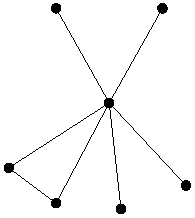
\includegraphics[height=2.6cm]{grafo-1.pdf} &
            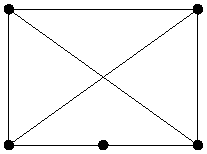
\includegraphics[height=2.6cm]{grafo-2.pdf} &
            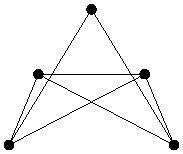
\includegraphics[height=2.6cm]{grafo-3.pdf} &
            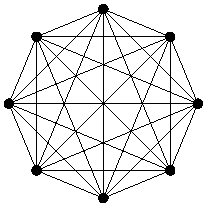
\includegraphics[height=2.6cm]{grafo-4.pdf} \\
            Grafo 1 & Grafo 2 & Grafo 3 & Grafo 4
        \end{tabular}
    \end{center}

    En lugar de dar una imagen, podemos describir un grafo enumerando sus vértices y aristas. Los siguientes datos
    describen por completo un grafo.

    \begin{quote}
        Vértices: $a,b,c,d,e$\\
        Aristas: $ab,ad,ae,bc,cd,ce,de$
    \end{quote}

    Este grafo tiene cinco vértices ($a$, $b$, $c$, $d$ y $e$) y siete aristas (entre los vértices $a$ y $b$, $a$ y $d$, y
    así sucesivamente). Obsérvese que tanto el Grafo 2 como el Grafo 3 se ajustan a esta descripción. Consideramos al Grafo
    2 y al Grafo 3 como dos representaciones del mismo grafo.\\
    Podemos ver cualquier grafo como una estructura $G$ de la siguiente manera. El conjunto subyacente $U$ de $G$ es el
    conjunto de vértices. El vocabulario $\VV_{G}$ de $G$ consiste en una única relación binaria $R$. La estructura $G$
    interpreta $R$ como la relación de adyacencia. Es decir, para elementos $a$ y $b$ de $U$, $G\models R(a,b)$ si y solo si
    el grafo tiene una arista entre los vértices $a$ y $b$.\\
    Cada uno de los grafos anteriores modela cada una de las siguientes dos $\VV_{G}$-sentencias.
    \begin{gather*}
        \forall x\neg R(x,x)\\
        \forall x\forall y(R(x,y)\ssi R(y,x))
    \end{gather*}
    La primera de estas sentencias dice que la relación binaria $R$ no es reflexiva (ningún vértice es adyacente a sí
    mismo). La segunda sentencia dice que $R$ es simétrica. De ahora en adelante, cuando hablemos de un \textit{grafo},
    queremos decir una $\VV_{G}$-estructura que modela las dos sentencias anteriores. Nuestra noción de \comillas{grafo} se
    describe con más precisión, en términos de la teoría de grafos, como un \comillas{grafo no dirigido sin aristas
    múltiples ni lazos.}\\
    Los Grafos 1 a 4 también modelan la sentencia $\forall x\exists yR(x,y)$, que afirma que cada vértice es adyacente a
    algún otro vértice. Sin embargo, esto no es cierto para todos los grafos. Por ejemplo, considere el siguiente grafo:

    \begin{center}
        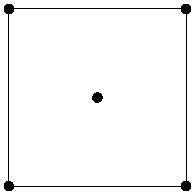
\includegraphics[height=2.6cm]{grafo-5.pdf}\\
        Grafo 5
    \end{center}

    El vértice en el centro del cuadrado no es adyacente a ningún vértice. Por lo tanto, este grafo modela
    $\exists x\forall y\neg R(x,y)$, que es equivalente a la negación de $\forall x\exists yR(x,y)$. Cualquier grafo que
    contenga más de un vértice y modele esta negación no puede ser \textit{conexo}. Definimos ahora esta terminología.

    \begin{definicion}\label{def:camino-grafo}
        Para cualesquiera vértices $a$ y $b$ de un grafo, un \textit{camino} de $a$ a $b$ es una sucesión de vértices que
        comienza con $a$ y termina con $b$, tal que cada vértice, salvo $a$, es adyacente al vértice anterior en la
        sucesión.
    \end{definicion}

    \begin{definicion}[Conexo]\label{def:conexo}
        Un grafo es \textit{conexo} si para cualesquiera dos vértices $a$ y $b$ de $G$, existe un camino de $a$ a $b$.
    \end{definicion}

    Cada uno de los Grafos 1 a 4 es conexo. Dado que cada uno tiene más de un vértice, cada uno modela
    $\forall x\exists yR(x,y)$. Por otro lado, ninguno de estos grafos modela $\exists x\forall yR(x,y)$. Esta sentencia
    afirma que existe un vértice adyacente a todo vértice. Dado que ningún vértice es adyacente a sí mismo, ningún grafo
    modela esta sentencia (es decir, la negación de $\exists x\forall yR(x,y)$ es consecuencia de $\forall x\neg R(x,x)$).
    Sin embargo, el Grafo 1 contiene un vértice que es adyacente a todo vértice distinto de sí mismo. Esto puede expresarse
    en lógica de primer orden de la siguiente manera:
    \begin{equation*}
        \exists x\forall y(\neg(x=y)\rightarrow R(x,y)).
    \end{equation*}
    El Grafo 4 también modela esta sentencia.\\
    Para distinguir el Grafo 1 del Grafo 4, podemos decir que el Grafo 1 contiene un \textit{único} vértice que es
    adyacente a todo vértice distinto de sí mismo. Esto puede expresarse como una sentencia de la lógica de primer orden.
    Para simplificar esta sentencia, sea $\varphi(x)$ la fórmula $\forall y(\neg(x=y)\rightarrow R(x,y))$. Para cualquier
    grafo $G$ y cualquier vértice $a$ de $G$, $G\models\varphi(a)$ si y solo si $a$ es adyacente a todo vértice de $G$
    distinto de $a$ mismo. La siguiente sentencia dice que existe un único elemento así:
    \begin{equation*}
        \exists y\varphi(y)\wedge\forall z(\varphi(z)\rightarrow(z=y)).
    \end{equation*}
    Esta sentencia distingue al Grafo 1 de los Grafos 2 a 4.\\
    El Grafo 4, por otro lado, se caracteriza por la siguiente sentencia, que dice que $\varphi(x)$ se cumple para todo
    vértice $x$.
    \begin{equation*}
        \forall x\forall y(\neg(x=y)\rightarrow R(x,y)).
    \end{equation*}
    A cualquier grafo que modele esta sentencia se le llama una \textit{clica} (o \textit{grafo completo}). A la clica que
    tiene $n$ vértices se le llama la $n$-clica y se denota por $K_{n}$. Así, el Grafo 4 es la 8-clica $K_{8}$. Obsérvese
    que, cuando se especifica $n$, usamos el artículo definido al referirnos a la $n$-clica. Esto se debe a que dos
    $n$-clicas cualesquiera son esencialmente la misma. Más precisamente, son isomorfas.

    \begin{definicion}[Isomorfismo de grafos]\label{def:isomorfismo-grafos}
        Se dice que los grafos $G_{1}$ y $G_{2}$ son \textit{isomorfos} si existe una correspondencia biunívoca $f$ del
        conjunto de vértices de $G_{1}$ sobre el conjunto de vértices de $G_{2}$ tal que, para cualesquiera vértices $a$ y
        $b$ de $G_{1}$, $a$ y $b$ son adyacentes en $G_{1}$ si y solo si $f(a)$ y $f(b)$ son adyacentes en $G_{2}$. A tal
        función $f$ se le llama un \textit{isomorfismo}.
    \end{definicion}

    Los grafos isomorfos son esencialmente el mismo.

    \begin{ejemplo}\label{ej:grafos-isomorfos}
        Considere los siguientes dos grafos.

        \begin{quote}
            Grafo $G$:\\
            Vértices: $a,b,c,d$\\
            Aristas: $ab,bc,cd,ad$.
        \end{quote}

        \begin{quote}
            Grafo $H$:\\
            Vértices: $w,x,y,z$\\
            Aristas: $wx,wy,xz,yz$.
        \end{quote}

        La función $f$ definida por
        \begin{equation*}
            f(a)=w,\quad f(b)=x,\quad f(c)=z,\quad\text{y}\quad f(d)=y
        \end{equation*}
        es un isomorfismo de $G$ sobre $H$. Ambos grafos pueden representarse como cuadrados. La única diferencia entre
        $G$ y $H$ son las letras usadas para representar los vértices.
    \end{ejemplo}

    Hemos exhibido una $\VV_{G}$-sentencia que distingue al Grafo 1 del Grafo 4. Podemos hacer algo mucho mejor que esto.
    Existe una $\VV_{G}$-sentencia que distingue al Grafo 1 de todos los grafos que no son isomorfos al Grafo 1. Es decir,
    existe una $\VV_{G}$-sentencia $\varphi_{G}$ tal que, para cualquier grafo $H$, $H\models\varphi_{G}$ si y solo si $H$
    es isomorfo a $G$. Demostramos esto en la Sección 2.6 como Proposición \ref{prop:sentencia-caracteriza-grafo-finito}. En
    este sentido, la lógica de primer orden es un lenguaje poderoso para describir grafos finitos.\\
    En otro sentido, sin embargo, la lógica de primer orden no es un lenguaje poderoso. Propiedades básicas de la teoría de
    grafos no pueden expresarse usando lógica de primer orden. Por ejemplo, no existe ninguna sentencia de primer orden que
    diga que un grafo tiene un número par de vértices. Tampoco puede la lógica de primer orden decir que un grafo es
    conexo. Recordemos que la sentencia $\forall x\exists yR(x,y)$ se cumple en cualquier grafo conexo que tenga más de un
    vértice. Sin embargo, el hecho de que esta sentencia se cumpla en una estructura no significa que sea conexa. No existe
    una $\VV_{G}$-sentencia $\varphi$ tal que $G\models\varphi$ si y solo si $G$ es un grafo conexo. Estas y otras
    limitaciones de la lógica de primer orden se discuten en la Sección 4.7.

    \subsection{Bases de datos relacionales}

    Las bases de datos relacionales proporcionan ejemplos concretos de estructuras. Cualquier colección de datos puede
    verse como una base de datos, ya sea un directorio telefónico, un catálogo de discos, o un árbol genealógico. Una base
    de datos relacional se presenta como un conjunto de tablas. Por ejemplo, las tres tablas siguientes forman una base de
    datos relacional (Tablas 2.1 a 2.3).\\
    Describimos ahora una estructura $D$ que representa esta base de datos relacional. El conjunto subyacente de $D$
    consiste en todos los elementos que aparecen como entrada en alguna columna de una tabla. Así, este conjunto contiene
    13 nombres y cuatro fechas.

    % ----- Tabla 2.1 -----
    \begin{table}[htbp]
        \centering
        \caption{Tabla de padres}
        \renewcommand{\arraystretch}{1.3}
        \begin{tabular}{c c}
            Padre/Madre & Hijo/Hija\\
            \hline
            Ray & Ken\\
            Ray & Sue\\
            Sue & Tim\\
            Dot & Jim\\
            Bob & Jim\\
            Bob & Liz\\
            Jim & Tim\\
            Sue & Sam\\
            Jim & Sam\\
            Zelda & Max\\
            Sam & Max\\
        \end{tabular}
    \end{table}

    % ----- Tabla 2.2 -----
    \begin{table}[htbp]
        \centering
        \caption{Tabla de mujeres}
        \renewcommand{\arraystretch}{1.3}
        \begin{tabular}{c}
            Mujeres\\
            \hline
            Dot\\
            Zelda\\
            Liz\\
            Sue\\
        \end{tabular}
    \end{table}

    % ----- Tabla 2.3 -----
    \begin{table}[htbp]
        \centering
        \caption{Tabla de cumpleaños}
        \renewcommand{\arraystretch}{1.3}
        \begin{tabular}{c c}
            Persona & Cumpleaños\\
            \hline
            Ann & 5 de agosto\\
            Leo & 8 de agosto\\
            Max & 28 de julio\\
            Sam & 1 de agosto\\
            Sue & 24 de julio\\
        \end{tabular}
    \end{table}

    El vocabulario $\VV$ de $D$ consiste en una relación $n$-aria por cada tabla, donde $n$ es el número de columnas de la
    tabla. Es decir, el vocabulario contiene una relación unaria $F$ y relaciones binarias $P$ y $B$ correspondientes a las
    tablas de Mujeres, Padres y Cumpleaños.\\
    La $\VV$-estructura $D$ interpreta estas relaciones como filas de las tablas. Por ejemplo, $D\models B(a,b)$ si y solo
    si \comillas{$ab$} es una fila de la tabla de Cumpleaños. Esto describe por completo la $\VV$-estructura $D$. Por
    ejemplo, vemos que
    \begin{gather*}
        D\models F(\text{Dot}),\quad D\models P(\text{Zelda},\text{Max}),\quad\text{y}\\
        D\models\neg B(\text{Zelda},\text{28 de julio}).
    \end{gather*}
    Además de $B$, $F$ y $P$, podemos definir fórmulas de primer orden que expresan otras relaciones diversas en $D$. Por
    ejemplo, la fórmula $\neg F(x)$ dice que $x$ es hombre. La fórmula $\exists z(P(x,z)\wedge P(z,y))$ dice que $x$ es
    abuelo o abuela de $y$. La conjunción de esta fórmula con $F(x)$ dice que $x$ es abuela de $y$. La fórmula
    $\exists yB(x,y)$ dice que $x$ es una fecha, y la negación de esta fórmula dice que $x$ es una persona. La fórmula
    $\exists z(B(x,z)\wedge B(y,z))$ afirma que $x$ y $y$ cumplen años el mismo día. No hay fin a las relaciones que pueden
    definirse (véase el Ejercicio 2.2).\\
    Volvemos a este ejemplo al final del Capítulo 3, donde discutimos Prolog. Prolog es un lenguaje de programación basado
    en la lógica de Horn de primer orden que puede usarse para presentar y consultar cualquier base de datos relacional.

    \subsection{Órdenes lineales}

    A continuación, examinamos algunas estructuras en el vocabulario $\VV_{<}$ que consiste únicamente en la relación
    binaria $<$. En lugar de usar la notación \comillas{$<(x,y)$,} usamos la más familiar \comillas{$x<y$} para expresar
    que la relación binaria $<$ se cumple para el par ordenado $(x,y)$. Como indica nuestra elección de símbolos, cada una
    de las estructuras que consideramos interpreta $<$ como \comillas{menor que.}\\
    Consideramos cuatro $\VV_{<}$-estructuras denotadas por $\N_{<}$, $\Z_{<}$, $\Q_{<}$ y $\R_{<}$. Para definir cada
    estructura, debemos indicar cuál es el conjunto subyacente y cómo se interpretan los símbolos. Los conjuntos
    subyacentes de las estructuras anteriores son, en orden, los números naturales, los enteros, los números racionales y
    los números reales. Cada una de estas estructuras interpreta $<$ de la manera usual. Podemos presentar estas
    estructuras de forma más concisa como sigue:

    \begin{itemize}
        \item[$\bullet$] $\N_{<}=(\N\mid<)$
        \item[$\bullet$] $\Z_{<}=(\Z\mid<)$
        \item[$\bullet$] $\Q_{<}=(\Q\mid<)$
        \item[$\bullet$] $\R_{<}=(\R\mid<)$.
    \end{itemize}

    Estas cuatro estructuras tienen mucho en común. Todas son $\VV_{<}$-estructuras y cada una de ellas modela las
    siguientes $\VV_{<}$-sentencias:
    \begin{gather*}
        \forall x\forall y((x<y)\rightarrow\neg(y<x))\\
        \forall x(\neg(x<x))\\
        \forall x\forall y((x<y)\vee(y<x)\vee(x=y))\\
        \forall x\forall y\forall z(((x<y)\wedge(y<z))\rightarrow(x<z)).
    \end{gather*}
    Tomadas en conjunto, estas sentencias dicen que $<$ ordena linealmente al conjunto subyacente. Cada una de las cuatro
    estructuras modela cada una de estas cuatro sentencias. Sin embargo, esto no es cierto para todas las
    $\VV_{<}$-sentencias. Sea $\varphi$ la sentencia $\forall x\exists y(y<x)$, que dice que no hay un elemento más pequeño.
    Claramente, $\R_{<}$, $\Q_{<}$ y $\Z_{<}$ son modelos de $\varphi$. Sin embargo, $\N_{<}$ sí tiene un elemento más
    pequeño, a saber, 1. Así, $\N_{<}$ no modela $\varphi$; más bien, $\N_{<}$ modela la sentencia
    $\exists x\forall y\neg(y<x)$, que afirma que existe un elemento más pequeño. Llamemos $\theta$ a esta sentencia.
    Obsérvese que $\theta$ es equivalente a $\neg\varphi$. La sentencia $\theta$ distingue a $\N_{<}$ de los otros tres
    modelos.\\
    A continuación, busquemos una sentencia de primer orden que distinga a $\Z_{<}$ de las otras tres estructuras.
    Observemos que $\Z_{<}$ no tiene un elemento más pequeño y no es densa. Un conjunto linealmente ordenado es
    \textit{denso} si entre cualesquiera dos elementos hay otro elemento. Esta propiedad puede expresarse en lógica de
    primer orden mediante la siguiente $\VV_{<}$-sentencia
    \begin{equation*}
        \forall x\forall y((x<y)\rightarrow\exists z((x<z)\wedge(z<y))).
    \end{equation*}
    Llamemos $\delta$ a esta sentencia. Tanto $\Q_{<}$ como $\R_{<}$ modelan $\delta$. Entre cualesquiera dos números
    racionales $a$ y $b$ existen infinitos números racionales [$(a+b)/2$, por ejemplo]. Lo mismo es cierto para los números
    reales. Sin embargo, los enteros no son densos. Entre 1 y 2 no hay otros enteros. Así, $\Z_{<}\models\neg\delta$. La
    $\VV_{<}$-sentencia $\varphi\wedge\neg\delta$ distingue a $\Z_{<}$ de las otras tres estructuras.\\
    Supongamos ahora que queremos distinguir entre $\Q_{<}$ y $\R_{<}$. Podríamos usar el hecho de que $\R_{<}$ es más
    grande que $\Q_{<}$. (En la siguiente sección discutimos en detalle el tamaño de una estructura y mostramos que, en
    cierto sentido preciso, hay más números reales que números racionales.) Otra característica distintiva es la
    completitud del orden. Un orden lineal es \textit{completo en el orden} si no puede partirse en dos intervalos
    abiertos. El conjunto de los números racionales, por ejemplo, es la unión de los intervalos $(-\infty,\sqrt{2})$ y
    $(\sqrt{2},\infty)$. Los paréntesis \comillas{(} y \comillas{)} indican que los intervalos no contienen los extremos
    (esto es lo que queremos decir con \comillas{abierto}). Dado que $\sqrt{2}$ no es un número racional, todo número
    racional está en uno de estos dos intervalos. Así, $\Q_{<}$ no tiene completitud en el orden. La estructura $\R_{<}$,
    por otro lado, sí tiene completitud en el orden. Esta es una característica distintiva de los números reales.\\
    Sin embargo, si intentamos hallar una $\VV_{<}$-sentencia que distinga a $\R_{<}$ de $\Q_{<}$, fracasaremos. Para toda
    $\VV_{<}$-sentencia $\varphi$, $\R_{<}\models\varphi$ si y solo si $\Q_{<}\models\varphi$. Damos una demostración
    elemental de esto en la Sección 5.2. Nuestro lenguaje de primer orden es demasiado débil para expresar cualquier
    diferencia entre estas estructuras. Señalamos que $\R_{<}$ es completa en el orden mientras que $\Q_{<}$ no lo es, pero
    no podemos expresar esto mediante una sentencia de primer orden (inténtelo). Más bien, la completitud del orden es un
    concepto de segundo orden. En lógica de segundo orden podemos expresar cosas como \comillas{no existen dos
    subconjuntos tales que\dots} También señalamos que $\R$ es más grande que $\Q$, pero, como veremos en el Capítulo 4, la
    lógica de primer orden no puede distinguir entre un número infinito y otro. Tanto $\Q_{<}$ como $\R_{<}$ son infinitas,
    y eso es todo lo que la lógica de primer orden puede decir. Desde el punto de vista de las $\VV_{<}$-sentencias, las
    estructuras $\R_{<}$ y $\Q_{<}$ son idénticas.

    \subsection{Sistemas numéricos}

    Aunque la lógica de primer orden no puede distinguir entre las $\VV_{<}$-estructuras $\Q_{<}$ y $\R_{<}$, sí puede
    distinguir entre los números reales y los números racionales en vocabularios distintos de $\VV_{<}$. Consideremos el
    vocabulario de la aritmética $\{+,\cdot,0,1\}$, con funciones binarias $+$ y $\cdot$, y constantes $0$ y $1$. Sea
    $\VV_{ar}$ este vocabulario, y consideremos las siguientes $\VV_{ar}$-estructuras:

    \begin{itemize}
        \item[$\bullet$] $A=(\Z\mid+,\cdot,0,1)$,
        \item[$\bullet$] $Q=(\Q\mid+,\cdot,0,1)$,
        \item[$\bullet$] $R=(\R\mid+,\cdot,0,1)$,
        \item[$\bullet$] $C=(\C\mid+,\cdot,0,1)$.
    \end{itemize}

    Los conjuntos subyacentes de estas estructuras son, en orden, los enteros, los números racionales, los números reales y
    los números complejos. Cada una de estas estructuras interpreta los símbolos de $\VV_{ar}$ de la manera usual.\\
    En lugar de usar la notación formal \comillas{$+(x,y)=z$,} usamos la más convencional \comillas{$x+y=z$.} Del mismo
    modo, escribimos $x\cdot y$ en lugar de $\cdot(x,y)$. Dejamos que 2 abrevie $(1+1)$, $x^{2}$ abrevie $x\cdot x$, y así
    sucesivamente. Cualquier polinomio que tenga números naturales como coeficientes es un $\VV_{ar}$-término. Ecuaciones
    como (por ejemplo)
    \begin{equation*}
        x^{5}-9x+3=0
    \end{equation*}
    son $\VV_{ar}$-fórmulas. De nuevo, 3 y $x^{5}$ no son símbolos de $\VV_{ar}$; son abreviaturas de los $\VV_{ar}$-términos
    $(1+(1+1))$ y $x\cdot(x\cdot(x\cdot(x\cdot x)))$, respectivamente.\\
    Todavía no podemos expresar la completitud del orden en este vocabulario, pero sí podemos distinguir entre las
    estructuras $R$ y $Q$. La $\VV_{ar}$-sentencia $\exists x(x^{2}=1+1)$ afirma la existencia de $\sqrt{2}$. Se sigue que
    $R$ modela esta sentencia y $Q$ no. Del mismo modo, la ecuación $2x+3=0$ tiene solución en $Q$ pero no en $A$. Así,
    $Q\models\exists x(2x+3=0)$, mientras que $A\models\neg\exists x(2x+3=0)$.\\
    Para progresar de $\N$ a $\Z$, a $Q$, agregamos soluciones para cada vez más polinomios. Llegamos al final del camino
    con los números complejos $C$. Los números complejos se obtienen agregando a los reales la solución $i=\sqrt{-1}$ de la
    ecuación $x^{2}+1=0$. La $\VV_{ar}$-sentencia $\exists x(x^{2}+1=0)$ distingue a $C$ de las demás estructuras de nuestra
    lista. El conjunto $\C$ consiste en todos los números de la forma $a+bi$ donde $a$ y $b$ son ambos números reales. El
    Teorema Fundamental del Álgebra establece que, para cualquier polinomio no constante $P(x)$ con coeficientes en $\C$, la
    ecuación $P(x)=0$ tiene solución en $\C$ (esto es cierto incluso para polinomios de más de una variable). Así, no hay
    necesidad de extender a un sistema numérico más grande. En virtud de agregar una solución de $x^{2}+1=0$ a $\R$, hemos
    agregado una solución para todo polinomio.\\
    Los nombres de estos sistemas numéricos reflejan sesgos históricos. Los números de conteo $1,2,3,\dots$ son los números
    \comillas{naturales} a considerar en matemáticas. Los números negativos no son naturales, la raíz cuadrada de 2 es
    irracional, y la raíz cuadrada de $-1$ es imaginaria. Los nombres sugieren que las cosas se vuelven más complicadas a
    medida que avanzamos de los números \comillas{naturales} a los números \comillas{complejos.} Desde el punto de vista de
    la lógica de primer orden, sin embargo, esto está al revés. La estructura $C$ es la más simple. La estructura $R$ no es
    simple como $C$, pero sí tiene muchas propiedades deseables. Discutiremos las propiedades de estas dos estructuras en
    el Capítulo 5. La estructura $A$ no es tan agradable. La \comillas{$A$} representa \comillas{aritmética,} lo cual suena
    bastante elemental. Sin embargo, desde el punto de vista de la lógica de primer orden, $A$ es la más compleja.
    Investigamos la estructura $A$ en el Capítulo 8.

    \section{El tamaño de una estructura}

    Para cualquier conjunto $U$, $|U|$ denota el número de elementos de $U$. Para una $\VV$-estructura $M$, $|M|$ significa
    $|U_{M}|$, el número de elementos del conjunto subyacente $U_{M}$ de $M$. Nos referimos a $|M|$ como el
    \textit{tamaño} de $M$. Por ejemplo, si $M_{2}$ es el Grafo 2 de la Sección 2.4.1, entonces $|M_{2}|=5$. Si el conjunto
    subyacente de $M$ es infinito, podríamos simplemente escribir $|M|=\infty$ y no decir más, pero esto simplifica
    excesivamente la situación. Implica que dos conjuntos infinitos cualesquiera tienen el mismo tamaño. Este no es el
    caso. Para explicar esto, necesitamos decir con precisión qué queremos decir con \comillas{el mismo tamaño.}\\
    Sean $A$ y $B$ dos conjuntos finitos. Imagine cada conjunto como una caja de pelotas de ping-pong. Imagine meter la
    mano izquierda en la caja $A$ y la mano derecha en la caja $B$, y sacar una pelota de cada una. Repita este proceso.
    Meta las manos en las cajas y simultáneamente saque una pelota de cada una, y de nuevo, y de nuevo. Eventualmente, una
    de las cajas se vacía. Si la caja $B$ se vacía primero, entonces concluimos que la caja $A$ debía contener al menos
    tantas pelotas como la caja $B$ al principio. Es decir, $|B|\leq|A|$. Dado que $A$ y $B$ son finitos, esto es
    elemental. Para conjuntos infinitos tomamos esta idea como la definición de \comillas{$|B|$ es menor o igual que $|A|$.}

    \begin{definicion}\label{def:menor-igual-tamano}
        Sean $A$ y $B$ conjuntos. Definimos \comillas{$|B|\leq|A|$} de la siguiente manera: $|B|\leq|A|$ si existe una
        función inyectiva $f$ de $B$ en $A$.
    \end{definicion}

    La función de esta definición desempeña el mismo papel que nuestras manos derecha e izquierda en la discusión anterior.
    La definición exige que $f$ sea inyectiva y tenga dominio $B$. Dado cualquier elemento $b$ de $B$, la función
    \comillas{elige} un elemento $f(b)$ de $A$. Si existe tal función, concluimos que $|B|\leq|A|$.

    \begin{ejemplo}
        Sea $P$ el conjunto de todos los números naturales primos y sea $E$ el conjunto de todos los números naturales
        pares. Sea $f:P\rightarrow E$ definida por $f(p)=2p$. Esta función es inyectiva. Concluimos que $|P|\leq|E|$. Es
        decir, hay al menos tantos números pares como números primos.
    \end{ejemplo}

    \begin{ejemplo}\label{ej:NxN-mismo-tamano}
        Recordemos que $\N\times\N$ denota el conjunto de todos los pares ordenados $(m,n)$ de números naturales. Sea
        $f:\N\rightarrow\N\times\N$ definida por $f(n)=(n,1)$ para todo $n\in\N$. Esta función es inyectiva. Concluimos que
        $|\N|\leq|\N\times\N|$. Al lector no debería sorprenderle este hecho. Menos evidente es que lo contrario también es
        cierto. Considere la función $g:\N\times\N\rightarrow\N$ definida por $g(m,n)=2^{m}3^{n}$. Esta también es una
        función inyectiva. Así, no solo $|\N|$ es menor o igual que $|\N\times\N|$, sino que también $|\N\times\N|$ es menor
        o igual que $|\N|$. Naturalmente, concluimos que estos dos conjuntos tienen el mismo tamaño.
    \end{ejemplo}

    \begin{definicion}\label{def:mismo-tamano}
        Sean $A$ y $B$ conjuntos. Decimos que $A$ y $B$ tienen el \textit{mismo tamaño} y escribimos $|A|=|B|$ si tanto
        $|B|\leq|A|$ como $|A|\leq|B|$. Escribimos $|A|<|B|$ si $|A|\leq|B|$ y no es el caso que $|A|=|B|$.
    \end{definicion}

    Así pues, para mostrar que dos conjuntos $A$ y $B$ tienen el mismo tamaño, debemos exhibir una función inyectiva de
    $A$ a $B$ y una función inyectiva de $B$ a $A$. Basta con mostrar que existe una función $f$ de $A$ a $B$ (o de $B$ a
    $A$) que sea tanto inyectiva como sobreyectiva (dado que $f^{-1}$ también es inyectiva y sobreyectiva). A tal función
    se le llama una \textit{correspondencia biunívoca} o \textit{biyección}.

    \begin{ejemplo}
        Sea $\N$ el conjunto de los números naturales y sea de nuevo $E$ el conjunto de los números naturales pares. En
        cierto sentido hay \comillas{más} números naturales que números pares (dado que $E\subset\N$). Sin embargo, estos
        dos conjuntos tienen el mismo tamaño. Esto lo atestigua la función $f(x)=2x$, que define una biyección de $\N$
        sobre $E$.
    \end{ejemplo}

    \begin{ejemplo}\label{ej:R-I-mismo-tamano}
        Sea $\R$ los números reales y sea $I$ el intervalo $(0,1)$, el conjunto de todos los reales entre 0 y 1. La función
        $f:\R\rightarrow I$ definida por $f(x)=(2/\pi)\arctan x$ es una biyección de $\R$ sobre $I$. Así, $|\R|=|I|$.
    \end{ejemplo}

    Si los conjuntos $A$ y $B$ pueden ponerse en correspondencia biunívoca entre sí, entonces deben tener el mismo tamaño.
    El siguiente teorema afirma que el recíproco también es cierto. Si $|A|\leq|B|$ y $|B|\leq|A|$, entonces debe existir
    una biyección entre $A$ y $B$. Esto proporciona una definición alternativa de \comillas{mismo tamaño.}

    \begin{teorema}\label{thm:cantor-bernstein}
        Los conjuntos $A$ y $B$ tienen el mismo tamaño si y solo si existe una biyección de $A$ sobre $B$.
    \end{teorema}
    \begin{proof}
        Solo una dirección requiere demostración. Como ya señalamos, si existe una biyección entre $A$ y $B$, entonces $A$
        y $B$ deben tener el mismo tamaño. Demostramos ahora lo contrario: si $|A|=|B|$, entonces tal biyección
        necesariamente existe.\\
        Supongamos que $A$ y $B$ tienen el mismo tamaño. Por la definición de \comillas{mismo tamaño,} existen funciones
        inyectivas $f:A\rightarrow B$ y $g:B\rightarrow A$. Nuestro objetivo es exhibir una biyección $h:A\rightarrow B$.
        Antes de definir $h$, definimos algunas sucesiones.\\
        Dado cualquier $a\in A$, definimos una sucesión (posiblemente finita) $s_{a}$ de la siguiente manera. Sea $a_{1}=a$.
        Supongamos ahora que $a_{m}\in A$ se ha definido para algún $m\in\N$. Tomemos $b_{m}\in B$ tal que $g(b_{m})=a_{m}$.
        Si no existe tal $b_{m}$, entonces la sucesión termina. En caso contrario, si $b_{m}$ sí existe, la sucesión
        continúa. Tomemos $a_{m+1}\in A$ tal que $f(a_{m+1})=b_{m}$. De nuevo, si no existe tal $a_{m+1}$, la sucesión
        termina. Obsérvese que la sucesión alterna entre elementos de $A$ y elementos de $B$. La sucesión $s_{a}$ puede
        representarse de la siguiente manera:
        \begin{equation*}
            a_{1}\xleftarrow{g}b_{1}\xleftarrow{f}a_{2}\xleftarrow{g}b_{2}\xleftarrow{f}a_{3}\xleftarrow{g}b_{3}\cdots
        \end{equation*}
        Hay tres posibilidades para la sucesión $s_{a}$. O bien termina en algún elemento $a_{i}\in A$, o bien termina en
        algún elemento $b_{i}\in B$, o bien nunca termina. Estas tres posibilidades dividen al conjunto $A$ en tres
        subconjuntos.

        \begin{itemize}
            \item[$\bullet$] Sea $A_{A}$ el conjunto de todos los $a\in A$ tales que $s_{a}$ termina en $A$.
            \item[$\bullet$] Sea $A_{B}$ el conjunto de todos los $a\in A$ tales que $s_{a}$ termina en $B$.
            \item[$\bullet$] Sea $A_{N}$ el conjunto de todos los $a\in A$ tales que $s_{a}$ nunca termina.
        \end{itemize}

        De manera similar, podemos definir sucesiones $s_{b}$ que comienzan con $b\in B$ y dividen a $B$ de la siguiente
        manera:

        \begin{itemize}
            \item[$\bullet$] Sea $B_{A}$ el conjunto de todos los $b\in B$ tales que $s_{b}$ termina en $A$.
            \item[$\bullet$] Sea $B_{B}$ el conjunto de todos los $b\in B$ tales que $s_{b}$ termina en $B$.
            \item[$\bullet$] Sea $B_{N}$ el conjunto de todos los $b\in B$ tales que $s_{b}$ nunca termina.
        \end{itemize}

        La función $f$, restringida a $A_{A}$, es una biyección $f:A_{A}\rightarrow B_{A}$. Sabemos que $f$ es inyectiva.
        Para ver que es sobreyectiva, tomemos cualquier $b\in B_{A}$. Dado que la sucesión $s_{b}$ termina en $A$, debe
        existir $a\in A_{A}$ tal que $f(a)=b$. (En caso contrario, $s_{b}$ sería la sucesión de un solo elemento $b$).
        Del mismo modo, $g$, restringida a $B_{B}$, forma una biyección $g:B_{B}\rightarrow A_{B}$. Finalmente, $A_{N}$ y
        $B_{N}$ están en correspondencia biunívoca tanto por $g$ como por $f$. Una biyección $h:A\rightarrow B$ puede
        definirse ahora uniendo estas tres partes.
        \begin{equation*}
            h(a)=
            \begin{cases}
                f(a), & a\in A_{A}\\
                g^{-1}(a), & a\in A_{B}\\
                f(a), & a\in A_{N}
            \end{cases}
        \end{equation*}
    \end{proof}

    Para conjuntos finitos, el Teorema \ref{thm:cantor-bernstein} es elemental. Para determinar cuántas pelotas de
    ping-pong hay en una caja dada, ponemos las pelotas de ping-pong en correspondencia biunívoca con el conjunto
    $\{1,2,3,\dots,k\}$ para algún $k\in\N$ (es decir, las contamos). Decimos que dos cajas contienen el mismo número de
    pelotas de ping-pong si cada una puede ponerse en correspondencia biunívoca con el mismo conjunto $\{1,2,3,\dots,k\}$
    y, por lo tanto, entre sí. Si $A$ y $B$ son infinitos, podemos tener dificultad para visualizarlos como cajas de
    pelotas de ping-pong. Extrapolamos nuestras definiciones para conjuntos infinitos a partir de las definiciones
    correspondientes para conjuntos finitos. Además, empleamos la siguiente suposición.

    \begin{quote}
        \textbf{Suposición:} Si $A$ y $B$ son conjuntos, entonces $|A|\leq|B|$ o $|B|\leq|A|$.
    \end{quote}

    Para $A$ y $B$ finitos, esta suposición es un hecho que puede demostrarse. Si sacamos pelotas de ping-pong, una a la
    vez, de cada una de dos cajas dadas, eventualmente una (o ambas) de las cajas se vaciará. Debemos tener cuidado, sin
    embargo, al manejar cajas que contienen infinitas pelotas de ping-pong (véase el Ejercicio 2.43). Para $A$ y $B$
    infinitos, aceptamos esta suposición sin demostración. Es equivalente a un axioma de las matemáticas conocido como el
    Axioma de Elección.\\
    Se sigue de esta suposición que, para cualquier conjunto infinito $A$, $|\N|\leq|A|$. Esto da lugar a una dicotomía
    crucial de los conjuntos infinitos: o bien $|\N|=|A|$ o bien $|\N|<|A|$.

    \begin{definicion}\label{def:numerable}
        Un conjunto $A$ es \textit{numerable} si existe una biyección entre $A$ y $\N$.
    \end{definicion}

    \begin{definicion}\label{def:contable}
        Un conjunto $A$ es \textit{contable} si es finito o numerable. En caso contrario, $A$ es \textit{no contable}.
    \end{definicion}

    \begin{proposicion}\label{prop:Q-contable}
        El conjunto de los números racionales $\Q$ es contable.
    \end{proposicion}
    \begin{proof}
        Claramente, $|\N|\leq|\Q|$ (dado que $\N\subset\Q$). Recíprocamente, cada elemento no nulo de $\Q$ puede escribirse
        de manera única como una fracción reducida de números naturales multiplicada por $(-1)^{m}$ para $m=1$ o $2$. Sea
        $f:\Q\rightarrow\N$ definida por $f\left(\frac{a}{b}(-1)^{m}\right)=2^{a}3^{b}5^{m}$ donde $\frac{a}{b}$ está
        reducida. Además, sea $f(0)=0$. Entonces $f$ es una función inyectiva de $\Q$ en $\N$. Por definición,
        $|\Q|\leq|\N|$. Por lo tanto, $\Q$ y $\N$ tienen el mismo tamaño.
    \end{proof}

    De manera similar, mostramos en el Ejemplo \ref{ej:NxN-mismo-tamano} que $\N\times\N$ tiene el mismo tamaño que $\N$.
    Así, $\N\times\N$ es un conjunto contable. Usamos esto para demostrar el siguiente hecho útil.

    \begin{proposicion}\label{prop:union-contable-contable}
        La unión de una cantidad contable de conjuntos contables es contable.
    \end{proposicion}
    \begin{proof}
        Para cada $n\in\N$, sea $A_{n}$ un conjunto contable. Sea $U$ la unión de estos conjuntos. Si cada $A_{n}$ es
        numerable y son disjuntos entre sí, entonces $U$ es lo más grande posible. Supongamos que este es el caso. Así,
        cada $A_{n}$ puede enumerarse como $\{a_{1},a_{2},a_{3},\dots\}$. Sea $f(m,n)$ el $m$-ésimo elemento de la
        enumeración de $A_{n}$. Esto define una biyección $f:\N\times\N\rightarrow U$. Concluimos que $U$ tiene el mismo
        tamaño que $\N\times\N$. Dado que $\N\times\N$ es contable, también lo es $U$.
    \end{proof}

    Un ejemplo de un conjunto no contable lo proporciona el conjunto de todos los subconjuntos de $\N$. Para cualquier
    conjunto $A$, el conjunto de todos los subconjuntos de $A$ se llama el \textit{conjunto potencia} de $A$, denotado por
    $\PP(A)$. Mostramos que $|\PP(A)|$ es siempre estrictamente mayor que $|A|$.

    \begin{proposicion}\label{prop:potencia-mas-grande}
        Para cualquier conjunto $A$, $|A|<|\PP(A)|$.
    \end{proposicion}
    \begin{proof}
        Para mostrar que $|A|<|\PP(A)|$ debemos mostrar tanto que $|A|\leq|\PP(A)|$ como que $|A|\neq|\PP(A)|$.\\
        La función inyectiva $f:A\rightarrow\PP(A)$ definida por $f(a)=\{a\}$ (para cada $a\in A$) muestra que
        $|A|\leq|\PP(A)|$.\\
        Para mostrar que $|A|\neq|\PP(A)|$, debemos mostrar que no existe una biyección entre $A$ y $\PP(A)$. Sea $g$ una
        función inyectiva arbitraria de $A$ a $\PP(A)$. Mostramos que $g$ necesariamente no es sobreyectiva. (Obsérvese que
        la función inyectiva $f$ anterior tampoco es sobreyectiva.) Para cada elemento $a$ de $A$, o bien $a$ está en el
        conjunto $g(a)$, o bien $a$ no está en $g(a)$. Sea $X$ el conjunto de aquellos elementos $a$ de $A$ para los cuales
        $a$ no está en $g(a)$. Entonces $a\in X$ si y solo si $a\notin g(a)$. Para cada $a\in A$, no puede ser el caso que
        $g(a)=X$ (de lo contrario tendríamos $a\in X$ si y solo si $a\notin X$, lo cual es absurdo). Dado que $X$ no está
        en el rango de $g$, $g$ no es sobreyectiva. Dado que $g$ era arbitraria, concluimos que ninguna función inyectiva de
        $A$ a $\PP(A)$ es sobreyectiva.
    \end{proof}

    \begin{corolario}\label{cor:numerable-subconjuntos-no-contable}
        Todo conjunto numerable tiene una cantidad no contable de subconjuntos.
    \end{corolario}

    En particular, hay una cantidad no contable de subconjuntos de $\N$. Usamos este hecho para mostrar que hay una
    cantidad no contable de números reales.

    \begin{proposicion}\label{prop:R-no-contable}
        El conjunto de los números reales $\R$ es no contable.
    \end{proposicion}
    \begin{proof}
        Definimos una función inyectiva $f$ de $\PP(\N)$ en $\R$.\\
        Sea $X$ un elemento de $\PP(\N)$. Entonces, como subconjunto de los números naturales, $X$ contiene a lo sumo 10
        números de un dígito, a lo sumo 90 números de dos dígitos, a lo sumo 900 números de tres dígitos, y así
        sucesivamente. Sea $r_{X}$ el número real entre 0 y 1 descrito de la siguiente manera. Los primeros dos dígitos
        después del punto decimal representan el número de números de un dígito en $X$. A estos les siguen cada uno de los
        números de un dígito de $X$, enumerados en orden ascendente. Los siguientes dos dígitos en la expansión decimal de
        $r_{X}$ representan el número de números de dos dígitos en $X$. A estos les siguen la lista de los números de dos
        dígitos de $X$. Los siguientes tres dígitos indican cuántos números de tres dígitos hay en $X$, y así
        sucesivamente.\\
        Por ejemplo, sea $X=\{2,4,5,6,7,8,9,10,24,213,3246\}$. Hay 07 números de un dígito en $X$ (a saber, 2, 4, 5, 6, 7,
        8 y 9), hay 02 números de dos dígitos (a saber, 10 y 24), hay 001 número de tres dígitos (213), y 0001 número de
        cuatro dígitos (3246). Así, tenemos
        \begin{equation*}
            r_{X}=0.0724567890210240012130001324600000000\dots
        \end{equation*}
        El número $r_{X}$ contiene una descripción completa del conjunto $X$. Se sigue que la función
        $f:\PP(\N)\rightarrow\R$ definida por $f(X)=r_{X}$ es una función inyectiva. Por lo tanto, $|\PP(\N)|\leq|\R|$.
        Dado que $\PP(\N)$ es no contable, también lo es $\R$.
    \end{proof}

    A continuación mostramos que solo hay una cantidad contable de $\VV$-fórmulas para cualquier vocabulario contable $\VV$.

    \begin{proposicion}\label{prop:formulas-contables}
        Si el vocabulario $\VV$ es contable, entonces también lo es el conjunto de todas las $\VV$-fórmulas.
    \end{proposicion}
    \begin{proof}
        Definimos una función inyectiva $f$ del conjunto de todas las $\VV$-fórmulas en $\N$.\\
        Dado que $\VV$ es contable, podemos asignar un número natural distinto a cada símbolo que ocurre en una
        $\VV$-fórmula. Entonces, a cada $\VV$-fórmula le corresponde una sucesión finita de números naturales. Supongamos
        que una $\VV$-fórmula dada $\varphi$ tiene a $a_{1},a_{2},\dots,a_{m}$ como su sucesión asociada de números
        naturales. Definimos $f(\varphi)$ como el producto
        \begin{equation*}
            2^{a_{1}}\cdot 3^{a_{2}}\cdot 5^{a_{3}}\cdots p_{n}^{a_{n}}
        \end{equation*}
        donde $p_{n}$ denota el $n$-ésimo número primo. Recordemos dos hechos básicos sobre los números naturales: hay
        infinitos números primos y hay una única manera de factorizar cualquier número natural dado en primos. Así,
        podemos factorizar el número natural $f(\varphi)$ para recuperar la sucesión $a_{1},\dots,a_{n}$ y la fórmula
        $\varphi$. Se sigue que $f$ es una función inyectiva, como se requería.
    \end{proof}

    Por la Proposición \ref{prop:formulas-contables}, la mayoría de los subconjuntos de $\N$ no son definibles en ningún
    vocabulario contable. La misma idea usada para demostrar la Proposición \ref{prop:formulas-contables} puede usarse
    para mostrar que hay una cantidad contable de sentencias en español, o en cualquier otro idioma natural. Así, existen
    incontables números reales que eluden descripción en cualquier idioma natural. Del mismo modo, existen incontables
    subconjuntos de los números naturales que no pueden definirse. La siguiente proposición muestra que esto también es
    cierto para las funciones sobre los números naturales.

    \begin{proposicion}\label{prop:funciones-no-contables}
        El conjunto de todas las funciones de $\N$ en $\N$ es no contable.
    \end{proposicion}
    \begin{proof}
        Sea $F$ el conjunto de todas las funciones de $\N$ en $\N$. Mostramos que $|I|\leq|F|$. Recordemos que $I$ es el
        intervalo $(0,1)$ que consiste en los números reales entre 0 y 1. Por el Ejemplo \ref{ej:R-I-mismo-tamano}, $I$ y
        $\R$ tienen el mismo tamaño. Por la proposición anterior, $I$ es no contable. Sea $r$ un elemento arbitrario de $I$.
        Sea $f_{r}:\N\rightarrow\N$ definida dejando que $f_{r}(n)$ sea el $n$-ésimo dígito en la expansión decimal de $r$.
        Claramente, si $r_{1}$ y $r_{2}$ son números distintos en $I$, entonces $f_{r_{1}}$ y $f_{r_{2}}$ son funciones
        distintas. Por lo tanto, la función que asigna $f_{r}$ a la entrada $r$ es una función inyectiva de $I$ a $F$. Se
        sigue que $|I|\leq|F|$ y $F$ es no contable. (De hecho, hemos mostrado que existen incontables funciones de
        $\N$ al conjunto $\{0,1,2,3,4,5,6,7,8,9\}$.)
    \end{proof}

    Se dice que una función $f(x)$ es \textit{computable} si existe un programa de computadora que produce $f(x)$ al
    recibir $x$ como entrada. Aplicando la Proposición \ref{prop:formulas-contables} a los lenguajes de programación, vemos
    que solo hay una cantidad contable de posibles programas de computadora. Se sigue que existen incontables funciones de
    $\N$ en $\N$ que no pueden computarse. Esto también es cierto para las funciones sobre los reales. La mayoría de las
    funciones no son computables. Este hecho desafía la evidencia empírica. La mayoría de las funciones con las que estamos
    familiarizados (la mayoría de las funciones que uno encuentra en cálculo, digamos) son computables. La noción de
    computabilidad se discute en detalle en el Capítulo 7. En la Sección 7.6.1 daremos ejemplos de funciones que están
    definidas con precisión pero que no son computables.\\
    Al comienzo de esta sección dijimos que tener una sola noción de \comillas{infinito} es engañoso. Hemos sustituido
    esto por dos nociones. Un conjunto infinito es o bien contable o bien no contable. Muchos de los conjuntos infinitos que
    encontramos tienen el mismo tamaño que $\N$ o el mismo tamaño que $\R$. (Tanto $\PP(\N)$ como $F$ tienen el mismo
    tamaño que $\R$; véanse los Ejercicios 2.41 y 2.42.) Esta dicotomía sigue siendo tosca. La Proposición
    \ref{prop:potencia-mas-grande} garantiza la existencia de conjuntos no contables arbitrariamente grandes, así que
    tener una sola noción de \comillas{no contable} resulta ahora engañoso. En la Sección 4.2 introducimos los números
    cardinales para representar el tamaño de un conjunto y estudiamos con más profundidad la plétora de números no
    contables. Por ahora, terminamos nuestra digresión hacia el infinito y volvemos a nuestra discusión sobre las
    estructuras.

    \section{Relaciones entre estructuras}

    Consideramos ciertas relaciones que pueden o no darse entre dos estructuras de un mismo vocabulario.

    \subsection{Encajes}

    Sean $M$ y $N$ estructuras. La notación $f:M\rightarrow N$ se usa para denotar \comillas{$f$ es una función de $M$ en
    $N$.} Al usar esta notación, se entiende que $f$ no es un símbolo de los vocabularios de $M$ o de $N$. Cada función
    unaria del vocabulario de $M$ se interpreta como una función del universo de $M$ en sí mismo. Cuando hablamos de una
    función de $M$ en $N$, en realidad nos referimos a una función del conjunto subyacente de $M$ al conjunto subyacente de
    $N$. Es decir, a cada elemento $a$ del universo $U_{M}$ de $M$, $f$ le asigna un elemento $f(a)$ del universo $U_{N}$ de
    $N$. Nos interesa principalmente el caso en que, para algún vocabulario $\VV$, $M$ y $N$ son ambas $\VV$-estructuras y
    $f$ \textit{preserva} ciertas $\VV$-fórmulas.

    \begin{definicion}[Preservación]\label{def:preserva-formula}
        Sea $\VV$ un vocabulario y sean $M$ y $N$ $\VV$-estructuras. Una función $f:M\rightarrow N$ \textit{preserva} la
        $\VV$-fórmula $\varphi(\bar{x})$ si, para cada tupla $\bar{a}$ de elementos de $M$, $M\models\varphi(\bar{a})$
        implica $N\models\varphi(f(\bar{a}))$.
    \end{definicion}

    \begin{definicion}[Encaje]\label{def:encaje-literal-elemental}
        Sean $M$ y $N$ $\VV$-estructuras y sea $f:M\rightarrow N$ una función. Si $f$ preserva todas las $\VV$-fórmulas
        que son literales, entonces $f$ es un \textit{encaje literal} (o simplemente un \textit{encaje}). Si $f$ preserva
        todas las $\VV$-fórmulas, entonces $f$ es un \textit{encaje elemental}.
    \end{definicion}

    \begin{ejemplo}\label{ej:encaje-grafos}
        Considere los siguientes dos grafos:

        \begin{center}
            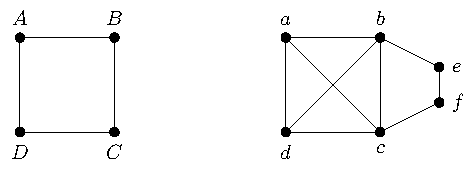
\includegraphics{grafos-encaje.pdf}
        \end{center}

        Sea $f:M\rightarrow N$ definida por
        \begin{equation*}
            f(A)=a,\ f(B)=b,\ f(C)=c,\quad\text{y}\quad f(D)=d.
        \end{equation*}
        Sea $g:M\rightarrow N$ definida por
        \begin{equation*}
            g(A)=b,\ g(B)=e,\ g(C)=d,\quad\text{y}\quad g(D)=f.
        \end{equation*}
        Entonces $g$ es un encaje literal y $f$ no lo es.
    \end{ejemplo}

    \begin{ejemplo}\label{ej:encaje-ordenes}
        Recordemos las estructuras $\N_{<}$, $\Z_{<}$, $\Q_{<}$ y $\R_{<}$ de la Sección 2.4.3.\\
        Sea $\mathrm{id}:\N_{<}\rightarrow\Z_{<}$ la función identidad definida por $\mathrm{id}(x)=x$. Este es un encaje
        literal. Dado que $\N_{<}\models\neg\exists x(x<0)$ y $\Z_{<}\models\exists x(x<0)$, este encaje no preserva la
        fórmula $\neg\exists x(x<y)$, y por lo tanto no es un encaje elemental.\\
        La función identidad $\mathrm{id}:\Z_{<}\rightarrow\Q_{<}$ también es un encaje literal que no es elemental (no
        preserva la fórmula $\neg\exists x(y<x\wedge x<z)$).\\
        La función identidad de $\Q_{<}$ a $\R_{<}$, por otro lado, es un encaje elemental. Esto se demostrará en el
        Capítulo 5.
    \end{ejemplo}

    A continuación mostramos que los encajes literales preservan necesariamente fórmulas que no son literales.

    \begin{definicion}[Fórmula sin cuantificadores]\label{def:formula-sin-cuantificadores}
        Una \textit{fórmula sin cuantificadores} es una fórmula en la que no ocurren los cuantificadores $\exists$ ni
        $\forall$.
    \end{definicion}

    \begin{definicion}[Fórmula existencial]\label{def:formula-existencial}
        Una \textit{fórmula existencial} es una fórmula de la forma $\exists y_{1}\exists y_{2}\dots\exists y_{m}
        \varphi(\bar{x},y_{1},y_{2},\dots,y_{m})$, donde $\varphi(\bar{x},\bar{y})$ es una fórmula sin cuantificadores y
        $m\geq 0$.
    \end{definicion}

    Mostramos que los encajes preservan las fórmulas existenciales. Primero demostramos la siguiente proposición relativa
    a las fórmulas sin cuantificadores.

    \begin{proposicion}\label{prop:encaje-preserva-sin-cuantificadores}
        Sea $f:M\rightarrow N$ un encaje. Entonces, para cualquier fórmula sin cuantificadores $\varphi(\bar{x})$ y
        cualquier tupla $\bar{a}$ de elementos del universo de $M$,
        \begin{equation*}
            M\models\varphi(\bar{a})\text{ si y solo si }N\models\varphi(f(\bar{a})).
        \end{equation*}
    \end{proposicion}
    \begin{proof}
        Procedemos por inducción sobre la complejidad de $\varphi$.\\
        Supongamos que $\varphi(\bar{x})$ es atómica. Entonces, dado que $f$ preserva literales, si $M\models\varphi(\bar{a})$,
        entonces $N\models\varphi(f(\bar{a}))$. Recíprocamente, si $N\models\varphi(f(\bar{a}))$ entonces, dado que
        $\neg\varphi(\bar{x})$ es un literal preservado por $f$, debe ser el caso que $M\models\varphi(\bar{a})$.\\
        Supongamos ahora que, para las fórmulas $\psi$ y $\theta$,
        \begin{equation*}
            M\models\psi(\bar{a})\text{ si y solo si }N\models\psi(f(\bar{a})),\quad\text{y}\quad
            M\models\theta(\bar{a})\text{ si y solo si }N\models\theta(f(\bar{a}))
        \end{equation*}
        para cualquier tupla $\bar{a}$ de elementos del universo de $M$. Esta es nuestra hipótesis de inducción. Dado que
        queremos demostrar la proposición solo para fórmulas sin cuantificadores, el paso inductivo, como en lógica
        proposicional, consta de tres partes correspondientes a $\neg$, $\wedge$ y $\equiv$. Debemos mostrar que
        $M\models\varphi(\bar{a})$ si y solo si $N\models\varphi(f(\bar{a}))$ cuando $\varphi$ es $\neg\psi$, cuando
        $\varphi$ es $\psi\wedge\theta$, y cuando $\varphi\equiv\psi$. Las dos primeras se siguen inmediatamente de la
        semántica de la lógica de primer orden, y la última se sigue de la definición de $\equiv$.
    \end{proof}

    \begin{proposicion}\label{prop:encaje-preserva-existenciales}
        Los encajes preservan las fórmulas existenciales.
    \end{proposicion}
    \begin{proof}
        Sea $f:M\rightarrow N$ un encaje y sea $\varphi(\bar{x})$ una fórmula existencial. Debemos mostrar que, para
        cualquier tupla $\bar{a}$ de elementos del universo $U_{M}$ de $M$, si $M\models\varphi(\bar{a})$ entonces
        $N\models\varphi(f(\bar{a}))$. Dado que $\varphi(\bar{x})$ es existencial, tiene la forma
        $\exists y_{1}\exists y_{2}\dots\exists y_{m}\varphi_{0}(\bar{x},y_{1},y_{2},\dots,y_{m})$, donde
        $\varphi_{0}(\bar{x},\bar{y})$ es una fórmula sin cuantificadores y $m\geq 0$.\\
        Por la semántica de $\exists$, $M\models\varphi(\bar{a})$ significa que $M\models\varphi_{0}(\bar{a},\bar{b})$ para
        alguna tupla $\bar{b}$ de elementos de $U_{M}$. Dado que $\varphi_{0}$ es sin cuantificadores, tenemos
        $N\models\varphi_{0}(f(\bar{a}),f(\bar{b}))$ por la proposición anterior. De nuevo por la semántica de $\exists$,
        $N\models\varphi(f(\bar{a}))$.
    \end{proof}

    Obsérvese que si $f:M\rightarrow N$ es un encaje literal, entonces, por la Proposición
    \ref{prop:encaje-preserva-sin-cuantificadores}, $M\models a=b$ si y solo si $N\models f(a)=f(b)$. Se sigue que todo
    encaje literal es necesariamente una función inyectiva. Obsérvese también que todo encaje elemental es un encaje
    literal. En general, \comillas{elemental} es un adjetivo mucho más fuerte que \comillas{literal.} Sin embargo, si $f$
    resulta ser sobreyectiva, entonces estas dos nociones coinciden.

    \begin{proposicion}\label{prop:encaje-biyectivo-elemental}
        Sean $M$ y $N$ $\VV$-estructuras. Si la función $f:M\rightarrow N$ es sobreyectiva, entonces $f$ es un encaje
        literal si y solo si $f$ es un encaje elemental.
    \end{proposicion}
    \begin{proof}
        Sea $f:M\rightarrow N$ un encaje literal que es sobreyectivo. Entonces $f^{-1}$ es una función inyectiva de $N$
        sobre $M$. Mostramos que tanto $f$ como $f^{-1}$ preservan cada $\VV$-fórmula. Es decir, para cada $\VV$-fórmula
        $\varphi(\bar{x})$ y cada tupla $\bar{a}$ de elementos de $M$, $M\models\varphi(\bar{a})$ si y solo si
        $N\models\varphi(f(\bar{a}))$. Demostramos esto por inducción sobre la complejidad de $\varphi(\bar{x})$. Si
        $\varphi(\bar{x})$ es atómica, esto es precisamente la Proposición \ref{prop:encaje-preserva-sin-cuantificadores}.\\
        Nuestra hipótesis de inducción es que tanto $f$ como $f^{-1}$ preservan las $\VV$-fórmulas $\psi$ y $\theta$. Si
        $\varphi$ es equivalente a $\psi$, entonces también es preservada por $f$ y $f^{-1}$. Además, si $\varphi$ es
        $\neg\psi$ o $\psi\wedge\theta$, entonces, por la semántica de $\neg$ y $\wedge$, $\varphi$ es preservada por $f$ y
        $f^{-1}$. Resta mostrar que $\varphi$ se preserva en el caso en que $\varphi$ es la fórmula $\exists y\psi$.\\
        Sea $\varphi(\bar{x})$ la fórmula $\exists y\psi(\bar{x},y)$. Primero mostramos que $f$ preserva $\varphi$.
        Supongamos que $M\models\varphi(\bar{a})$ para alguna tupla $\bar{a}$ de elementos de $M$. Entonces, por la
        semántica de $\exists$, $M\models\psi(\bar{a},b)$ para algún elemento $b$ de $M$. Dado que $\psi$ es preservada por
        $f$, $N\models\psi(f(\bar{a}),f(b))$. De nuevo por la semántica de $\exists$, $N\models\varphi(f(\bar{a}))$.\\
        Ahora mostramos que $f^{-1}$ preserva $\varphi$. Supongamos que $N\models\varphi(f(\bar{a}))$. Entonces, por la
        semántica de $\exists$, $N\models\psi(f(\bar{a}),c)$ para algún elemento $c$ de $N$. Dado que $f$ es sobreyectiva,
        $c=f(b)$ para algún elemento $b$ de $M$. Dado que $f^{-1}$ preserva $\psi$, $M\models\psi(\bar{a},b)$. Finalmente,
        de nuevo por la semántica de $\exists$, $M\models\varphi(\bar{a})$.
    \end{proof}

    \begin{definicion}[Isomorfismo]\label{def:isomorfismo-estructuras}
        Sean $M$ y $N$ $\VV$-estructuras. Una función de $M$ a $N$ es un \textit{isomorfismo} si es una correspondencia
        biunívoca que preserva toda $\VV$-fórmula. Si tal isomorfismo existe, decimos que $M$ y $N$ son \textit{isomorfas},
        denotado por $M\cong N$.
    \end{definicion}

    \begin{definicion}[Equivalencia elemental]\label{def:equivalencia-elemental}
        Sean $M$ y $N$ $\VV$-estructuras. Si $M$ y $N$ modelan las mismas $\VV$-sentencias, decimos que $M$ y $N$ son
        \textit{elementalmente equivalentes}, denotado por $M\equiv N$.
    \end{definicion}

    \begin{ejemplo}
        Las $\VV_{<}$-estructuras $\Q_{<}$ y $\R_{<}$ de la Sección 2.4.3 son elementalmente equivalentes.
    \end{ejemplo}

    \begin{proposicion}\label{prop:isomorfo-implica-equivalente}
        Sean $M$ y $N$ $\VV$-estructuras. Si $M\cong N$, entonces $M\equiv N$.
    \end{proposicion}
    \begin{proof}
        Sea $f:M\rightarrow N$ un isomorfismo. Entonces tanto $f$ como $f^{-1}$ preservan toda fórmula. En particular, para
        cualquier sentencia $\varphi$, $M\models\varphi$ si y solo si $N\models\varphi$.
    \end{proof}

    Si las $\VV$-estructuras $M$ y $N$ son elementalmente equivalentes, entonces no podemos distinguirlas usando lógica de
    primer orden. Además, si $M$ y $N$ son isomorfas, entonces son esencialmente la misma. La única diferencia entre
    estructuras isomorfas son los nombres dados a los elementos de los conjuntos subyacentes (recuerde el Ejemplo
    \ref{ej:grafos-isomorfos}).

    \subsection{Subestructuras}

    Si $B$ es un conjunto, $A\subset B$ significa que $A$ es un subconjunto de $B$. Si $N$ es una estructura, $M\subset N$
    significa que $M$ es una subestructura de $N$. Definimos ahora este concepto.

    \begin{definicion}[Subestructura]\label{def:subestructura}
        Para cualquier estructura $N$, $M$ es una \textit{subestructura} de $N$, denotado $M\subset N$, si
        \begin{enumerate}
            \item[1.] $M$ es una estructura que tiene el mismo vocabulario que $N$,
            \item[2.] el conjunto subyacente $U_{M}$ de $M$ es un subconjunto del conjunto subyacente $U_{N}$ de $N$, y
            \item[3.] $M$ interpreta el vocabulario de la misma manera que $N$ sobre $U_{M}$.
        \end{enumerate}
    \end{definicion}

    \begin{ejemplo}
        Recordemos las estructuras $\N_{<}$, $\Z_{<}$, $\Q_{<}$ y $R$ de la Sección 2.4.3. Tenemos
        $\N_{<}\subset\Z_{<}\subset\Q_{<}\subset R$. Del mismo modo, para las estructuras discutidas en la Sección 2.4.4,
        $A\subset Q\subset R\subset C$.
    \end{ejemplo}

    \begin{ejemplo}\label{ej:subgrafo-no-subestructura}
        Sea $G$ el siguiente grafo:

        \begin{quote}
            Vértices: $a,b,c,d,e$\\
            Aristas: $ab,ac,ad,ae,bc,cd,de$
        \end{quote}

        Si elegimos cualquier subconjunto de estos vértices y cualquier subconjunto de aristas que involucre a los vértices
        elegidos, obtenemos lo que en teoría de grafos se conoce como un \textit{subgrafo}.\\
        Sea $H$ el siguiente subgrafo de $G$.

        \begin{quote}
            Vértices: $a,b,c,d$\\
            Aristas: $ab,ad,bc,cd$
        \end{quote}

        Aunque $H$ es un subgrafo de $G$, $H$ no es una subestructura de $G$ (viendo a $G$ y a $H$ como
        $\VV_{G}$-estructuras). Dado que $G\models R(a,c)$ y $H\models\neg R(a,c)$, $H$ no interpreta la relación binaria
        $R$ de la misma manera que $G$ en el conjunto $\{a,b,c,d\}$. La noción de subestructura corresponde a la noción,
        propia de la teoría de grafos, de subgrafo inducido.
    \end{ejemplo}

    Sea $N$ una $\VV$-estructura y sea $U_{N}$ el conjunto subyacente de $N$. No todo subconjunto de $U_{N}$ puede servir
    como universo de una subestructura de $N$. Dado que una subestructura es en sí misma una $\VV$-estructura, debe
    interpretar cada constante y función de $\VV$. Dado que $N$ es una $\VV$-estructura, interpreta cada constante $c$ de
    $\VV$ como un elemento $a_{c}$ de $U_{N}$. Sea $C$ el subconjunto de $U_{N}$ definido por $C=\{a_{c}\mid c\text{ es una
    constante de }\VV\}$. Sea $f$ una función $n$-aria de $\VV$. Un subconjunto $D$ de $U_{N}$ es \textit{cerrado bajo $f$}
    si y solo si, para cada $n$-tupla $\bar{a}$ de elementos de $D$, $f(\bar{a})$ también es un elemento de $D$. Para que
    $D$ sea el universo de una subestructura de $N$, es necesario y suficiente que $D$ contenga a cada elemento de $C$ y
    sea cerrado bajo cada función de $\VV$.

    \begin{ejemplo}\label{ej:subestructuras-sucesor-relacion}
        Sea $N$ la estructura $(\N\mid S)$ que interpreta la relación binaria $S$ como la relación sucesor. Es decir, para
        cualesquiera $a$ y $b$ en $\N$, $N\models S(a,b)$ si y solo si $b=a+1$. Dado que el vocabulario no contiene ni
        constantes ni funciones, todo subconjunto de $\N$ es el universo de una subestructura de $N$. Se sigue que hay una
        cantidad no contable de subestructuras de $N$. Además, existen incontables subestructuras, ninguna de las cuales es
        isomorfa a otra. Dejamos la verificación de este hecho como Ejercicio 2.35.
    \end{ejemplo}

    \begin{ejemplo}\label{ej:subestructuras-sucesor-funcion}
        Sea $N$ la estructura $(\N\mid s)$ que interpreta la función unaria $s$ como la función sucesor. Es decir, para
        cualesquiera $a$ y $b$ en $\N$, $N\models s(a)=b$ si y solo si $b=a+1$. Solo aquellos subconjuntos de $\N$ que son
        cerrados bajo $s$ pueden servir como universo de una subestructura. Los subconjuntos cerrados de $\N$ son los
        conjuntos de la forma $\{n\mid n\geq d\}$ para algún $d\in\N$. Se sigue que hay una cantidad contable de
        subestructuras de $N$. Además, todas estas subestructuras son isomorfas. Así, solo hay una subestructura salvo
        isomorfismo.
    \end{ejemplo}

    \begin{ejemplo}
        Sea $N$ la estructura $(\N\mid s,1)$ que interpreta la función unaria $s$ como la función sucesor y la constante
        $1$ como el elemento 1 de $\N$. Si $D\subset\N$ es el universo de una subestructura de $N$, entonces $D$ debe
        contener a 1 y ser cerrado bajo la función $s$. Se sigue que $D$ debe ser todo $\N$. Por lo tanto, la única
        subestructura de $N$ es $N$ misma.
    \end{ejemplo}

    Una definición alternativa de subestructura la proporciona la noción de encaje.

    \begin{proposicion}\label{prop:subestructura-encaje-identidad}
        Sean $N$ y $M$ estructuras del mismo vocabulario. Entonces $M$ es una subestructura de $N$ si y solo si la función
        identidad $\mathrm{id}:M\rightarrow N$ definida por $\mathrm{id}(x)=x$ es un encaje.
    \end{proposicion}
    \begin{proof}
        Ejercicio \ref{ej:subestructura-encaje-identidad-completa}.
    \end{proof}

    Si $M\subset N$, decimos entonces, invirtiendo nuestro punto de vista, que $N$ es una \textit{extensión} de $M$.
    Obsérvese la distinción entre una \comillas{extensión} y una \comillas{expansión} de una estructura. Una estructura
    tiene tanto un conjunto subyacente como un vocabulario. Una expansión de una estructura tiene el mismo conjunto
    subyacente, pero el vocabulario puede aumentar. Una extensión de una estructura tiene el mismo vocabulario, pero el
    conjunto subyacente puede ampliarse.

    \begin{definicion}\label{def:preservada-extensiones}
        Se dice que la fórmula $\varphi(\bar{x})$ se \textit{preserva bajo extensiones} si, siempre que $M\subset N$ y
        $\bar{a}$ sea una tupla de elementos del universo de $M$, si $M\models\varphi(\bar{a})$ entonces
        $N\models\varphi(\bar{a})$.
    \end{definicion}

    \begin{definicion}\label{def:preservada-subestructuras}
        Se dice que la fórmula $\varphi(\bar{x})$ se \textit{preserva bajo subestructuras} si, siempre que $M\subset N$ y
        $\bar{a}$ sea una tupla de elementos del universo de $M$, si $N\models\varphi(\bar{a})$ entonces
        $M\models\varphi(\bar{a})$.
    \end{definicion}

    \begin{proposicion}\label{prop:sin-cuantificadores-preservada}
        Las fórmulas sin cuantificadores se preservan bajo subestructuras y bajo extensiones.
    \end{proposicion}
    \begin{proof}
        Esto se sigue inmediatamente de la Proposición \ref{prop:encaje-preserva-sin-cuantificadores}.
    \end{proof}

    \begin{proposicion}\label{prop:existencial-preservada-extensiones}
        Las fórmulas existenciales se preservan bajo extensiones.
    \end{proposicion}
    \begin{proof}
        Esto se sigue inmediatamente de la Proposición \ref{prop:encaje-preserva-existenciales}.
    \end{proof}

    En particular, las sentencias existenciales se preservan bajo extensiones. Intuitivamente, una sentencia existencial
    afirma que una fórmula sin cuantificadores $\varphi_{0}(\bar{y})$ se cumple para alguna tupla $\bar{y}$ de elementos
    del universo. Si esto es cierto en $M$ y $M\subset N$, entonces también debe ser cierto en $N$, ya que toda tupla de
    elementos del universo de $M$ es también una tupla de elementos del universo de $N$. Del mismo modo, si
    $\varphi_{0}(\bar{y})$ se cumple para todas las tuplas $\bar{y}$ de elementos del universo de $N$, entonces, en
    particular, se cumple para todos los elementos de cualquier subestructura de $N$. Así, las sentencias de la forma
    $\forall\bar{y}\varphi_{0}(\bar{y})$ se preservan bajo subestructuras.

    \begin{definicion}[Fórmula universal]\label{def:formula-universal}
        Una \textit{fórmula universal} es una fórmula de la forma
        \begin{equation*}
            \forall y_{1}\forall y_{2}\dots\forall y_{m}\varphi(\bar{x},y_{1},y_{2},\dots,y_{m}),
        \end{equation*}
        donde $\varphi(\bar{x},\bar{y})$ es una fórmula sin cuantificadores y $m\geq 0$.
    \end{definicion}

    \begin{proposicion}\label{prop:universal-preservada-subestructuras}
        Las fórmulas universales se preservan bajo subestructuras.
    \end{proposicion}
    \begin{proof}
        Ejercicio \ref{ej:universal-preservada-completa}.
    \end{proof}

    En el Capítulo 4 demostramos los recíprocos de estas proposiciones. Mostramos en la Sección 4.5.1 que si una fórmula
    $\varphi$ se preserva bajo subestructuras, entonces $\varphi$ es equivalente a una fórmula universal. Del mismo modo,
    si $\varphi$ se preserva bajo extensiones, entonces $\varphi$ es equivalente a una fórmula existencial.\\
    La noción de encaje elemental da lugar al siguiente fortalecimiento de la noción de subestructura.

    \begin{definicion}[Subestructura elemental]\label{def:subestructura-elemental}
        Sean $N$ y $M$ estructuras del mismo vocabulario. Entonces $M$ es una \textit{subestructura elemental} de $N$ (o,
        equivalentemente, $N$ es una \textit{extensión elemental} de $M$), denotado $M\prec N$, si y solo si la función
        identidad $\mathrm{id}:M\rightarrow N$ definida por $\mathrm{id}(x)=x$ es un encaje elemental.
    \end{definicion}

    Si $N$ es una extensión elemental de $M$, entonces, para cualquier fórmula $\varphi(\bar{x})$ y cualquier tupla
    $\bar{a}$ de elementos del universo de $M$, $M\models\varphi(\bar{a})$ si y solo si $N\models\varphi(\bar{a})$. Se
    sigue que si $M\prec N$, entonces $M\equiv N$. El recíproco de esto no se cumple. En el siguiente ejemplo, $M$ es una
    subestructura de $N$ y $M\equiv N$, pero $M$ no es una subestructura elemental de $N$.

    \begin{ejemplo}\label{ej:subestructura-no-elemental}
        Sea $N$ los números naturales con la función sucesor. Es decir, $N=(\N\mid s)$ del Ejemplo
        \ref{ej:subestructuras-sucesor-funcion}. Sea $M$ la subestructura de $N$ con universo $\{2,3,4,\dots\}$. Sea
        $f:N\rightarrow M$ definida por $f(n)=n+1$ para cada $n$ en $\N$. Entonces $f$ es un isomorfismo de $N$ sobre $M$.
        Tenemos tanto $M\subset N$ como $M\cong N$. Sin embargo, $M$ no es una subestructura elemental de $N$. Existe un
        encaje elemental de $M$ en $N$, pero no es la función identidad. En particular, sea $\varphi(x)$ la fórmula
        $\neg\exists y(s(y)=x)$, que dice que $x$ no tiene predecesor. Entonces $M\models\varphi(2)$, pero
        $N\models\neg\varphi(2)$.
    \end{ejemplo}

    \subsection{Diagramas}

    El concepto de diagrama (y, más específicamente, de diagrama elemental) de una $\VV$-estructura $M$ es un concepto
    fundamental que usaremos repetidamente en este libro (principalmente en el Capítulo 4). Intuitivamente, un diagrama de
    $M$ es un conjunto de sentencias de primer orden que, en conjunto, dicen \comillas{$M$ puede encajarse en mí.} Es
    decir, $M$ puede encajarse en cualquier modelo del diagrama de $M$. Del mismo modo, el diagrama elemental de $M$ es un
    conjunto de sentencias tal que $M$ puede encajarse elementalmente en cualquier modelo. Definimos ahora explícitamente
    estos conjuntos de sentencias. Recordemos que $\VV(M)$ denota la expansión de $\VV$ obtenida al agregar una constante
    por cada elemento del conjunto subyacente de $M$, y $M_{C}$ denota la expansión de $M$ a una $\VV(M)$-estructura que
    interpreta estas constantes de la manera natural.

    \begin{definicion}[Diagrama]\label{def:diagrama}
        Sea $M$ una $\VV$-estructura.\\
        El \textit{diagrama elemental} de $M$, denotado $ED(M)$, es el conjunto de todas las $\VV(M)$-sentencias que se
        cumplen en $M_{C}$.\\
        El \textit{diagrama literal} de $M$, denotado $D(M)$, es el conjunto de todos los literales de $ED(M)$. Con
        frecuencia nos referimos al diagrama literal de $M$ simplemente como el diagrama de $M$.
    \end{definicion}

    \begin{ejemplo}\label{ej:diagrama-grafo}
        Considere el grafo definido por la siguiente información:

        \begin{quote}
            Vértices: $a,b,c,d$\\
            Aristas: $ab,bc,cd,bd$.
        \end{quote}

        Sea $G$ la $\VV_{G}$-estructura representada por este grafo. El diagrama $D(G)$ contiene las fórmulas atómicas
        \begin{equation*}
            R(a,b),\quad R(b,c),\quad R(c,d),\quad\text{y}\quad R(b,d)
        \end{equation*}
        que expresan las aristas de $G$. También contiene las fórmulas atómicas negadas
        \begin{equation*}
            \neg R(a,c)\quad\text{y}\quad\neg R(a,d)
        \end{equation*}
        que expresan las aristas que no están en $G$. También hay fórmulas atómicas negadas que indican que $a$, $b$, $c$
        y $d$ son distintos:
        \begin{equation*}
            \neg(a=b),\ \neg(a=c),\ \neg(a=d),\ \neg(b=c),\ \neg(b=d),\quad\text{y}\quad\neg(c=d).
        \end{equation*}
        Obsérvese que $G$ puede encajarse en cualquier grafo que modele estos 12 literales de $D(G)$. Además, $D(G)$
        contiene los literales
        \begin{equation*}
            R(b,a),\quad R(c,b),\quad R(d,c),\quad\text{y}\quad R(d,b)
        \end{equation*}
        junto con
        \begin{equation*}
            \neg R(a,a),\ \neg R(b,b),\ \neg R(c,c),\ \neg R(d,d),
        \end{equation*}
        y
        \begin{equation*}
            a=a,\ b=b,\ c=c,\ d=d,\ \neg(b=a),\ \neg(c=a),\dots
        \end{equation*}
        y así sucesivamente. En total, hay 32 literales distintos (aunque redundantes) en $D(G)$. Obsérvese que $G$ puede
        encajarse en cualquier $\VV_{G}$-estructura que modele todas estas sentencias.
    \end{ejemplo}

    \begin{proposicion}\label{prop:equivalencia-encaje-diagrama}
        Sean $M$ y $N$ $\VV$-estructuras. Las siguientes son equivalentes:
        \begin{enumerate}
            \item[(i)] $M$ puede encajarse en $N$.
            \item[(ii)] $\widetilde{N}\models D(M)$ para alguna expansión $\widetilde{N}$ de $N$.
            \item[(iii)] $N'\cong N$ para alguna extensión $N'$ de $M$.
        \end{enumerate}
    \end{proposicion}
    \begin{proof}
        Sean $U_{M}$ y $U_{N}$ los conjuntos subyacentes de $M$ y $N$, respectivamente.\\
        Primero, mostramos que (iii) implica (i). Supongamos que $M\subset N'$ y $N'\cong N$. Sea $f:N'\rightarrow N$ un
        isomorfismo. Entonces $f$ restringida a $M$ es un encaje de $M$ en $N$.\\
        Para ver que (i) implica (ii), supongamos que $f:M\rightarrow N$ es un encaje. Sea $C=\{c_{m}:m\in U_{M}\}$
        constantes que no están en $\VV$. Sea $\VV(C)$ la expansión $\VV\cup C$ de $\VV$. Sea $\widetilde{N}$ la expansión
        de $N$ a una $\VV(C)$-estructura que interpreta cada $c_{m}\in C$ como el elemento $f(m)\in U_{N}$. Entonces
        $\widetilde{N}\models D(M)$.\\
        Finalmente, sea $\widetilde{N}$ como en (ii). Queremos mostrar que se cumple (iii). El conjunto $U_{M}$ podría no
        ser un subconjunto de $U_{N}$. Sin embargo, para cada $m\in U_{M}$, debe existir $m'\in U_{N}$ que $\widetilde{N}$
        interpreta como la constante $c_{m}$. Sea $U_{N'}$ el conjunto obtenido al reemplazar cada $m'\in U_{N}$ por $m$.
        Ahora $U_{M}\subset U_{N'}$. Sea $N'$ la $\VV$-estructura con conjunto subyacente $U_{N'}$ que interpreta $\VV$ de
        la misma manera que $N$. Entonces la función $f$ definida por $f(m)=m$ para $m\in U_{M}$ y $f(x)=x$ para
        $x\in U_{N}-U_{M}$ es un isomorfismo de $N$ sobre $N'$.
    \end{proof}

    Del mismo modo, tenemos lo siguiente.

    \begin{proposicion}\label{prop:equivalencia-encaje-elemental-diagrama}
        Sean $M$ y $N$ $\VV$-estructuras. Las siguientes son equivalentes:
        \begin{enumerate}
            \item[(i)] $M$ puede encajarse elementalmente en $N$.
            \item[(ii)] $\widetilde{N}\models ED(M)$ para alguna expansión $\widetilde{N}$ de $N$.
            \item[(iii)] $N'\cong N$ para alguna extensión elemental $N'$ de $M$.
        \end{enumerate}
    \end{proposicion}
    \begin{proof}
        Ejercicio \ref{ej:diagrama-elemental-completa}.
    \end{proof}

    Si $M$ es una estructura finita en un vocabulario finito, entonces $D(M)$ es finito. Se sigue que toda estructura
    finita queda completamente descrita por una única sentencia de la lógica de primer orden.

    \begin{proposicion}\label{prop:sentencia-caracteriza-grafo-finito}
        Sea $\VV$ un vocabulario finito. Para cualquier $\VV$-estructura finita $M$, existe una $\VV$-sentencia
        $\varphi_{M}$ tal que, para cualquier $\VV$-estructura $N$, $N\models\varphi_{M}$ si y solo si $N\cong M$.
    \end{proposicion}
    \begin{proof}
        Sea $\{a_{1},a_{2},\dots,a_{n}\}$ el conjunto subyacente de $M$. Sea $\varphi(\bar{a})$ la conjunción de las
        finitas sentencias de $D(M)$, donde $\bar{a}$ denota la $n$-tupla $(a_{1},a_{2},\dots,a_{n})$. Sea $\varphi(\bar{x})$
        la $\VV$-fórmula obtenida al reemplazar cada $a_{i}$ en $\varphi(\bar{a})$ por la variable $x_{i}$ (que suponemos
        no ocurre en $\varphi(\bar{a})$). Abreviamos la sentencia $\exists x_{1}\exists x_{2}\dots\exists x_{n}\varphi(\bar{x})$
        simplemente como $\exists\bar{x}\varphi(\bar{x})$.\\
        Sea $\psi_{n}$ la sentencia
        \begin{equation*}
            \forall x_{1}\forall x_{2}\dots\forall x_{n+1}\left(\bigvee_{i\neq j}(x_{i}=x_{j})\right)
        \end{equation*}
        que dice que, dados cualesquiera $n+1$ elementos, debe haber dos que sean iguales.\\
        Sea ahora $\varphi_{M}$ la sentencia $\psi_{n}\wedge\exists\bar{x}\varphi(\bar{x})$. Debemos verificar que esta
        sentencia funciona. Supongamos que $N\models\varphi_{M}$. Entonces, dado que $N\models\exists\bar{x}\varphi(\bar{x})$,
        $N$ contiene $n$ elementos $b_{1},\dots,b_{n}$ tales que $N\models\varphi(b_{1},\dots,b_{n})$. Por la Proposición
        \ref{prop:equivalencia-encaje-diagrama}, $M$ puede encajarse en $N$. Sea $f:M\rightarrow N$ un encaje. Dado que
        $N\models\psi_{n}$, $|N|\leq n$. Se sigue que $f$ debe ser sobreyectiva. Por la Proposición
        \ref{prop:encaje-biyectivo-elemental}, $f$ es elemental y, por lo tanto, un isomorfismo.
    \end{proof}

    \begin{corolario}\label{cor:isomorfo-sii-equivalente-finito}
        Si $M$ es finita, entonces, para cualquier estructura $N$, $M\cong N$ si y solo si $M\equiv N$.
    \end{corolario}

    Como mencionamos anteriormente, este corolario no es cierto para estructuras infinitas. Si $M$ es infinita, entonces
    existen muchas estructuras $N$ no isomorfas para las cuales $M\equiv N$. Esto se demuestra en el Capítulo 4. Dicho de
    otra manera, la lógica de primer orden no es capaz de describir por completo las estructuras infinitas. La lógica de
    primer orden es, en este sentido, un lenguaje débil. Irónicamente, como consecuencia de esta debilidad, la lógica de
    primer orden tiene muchas propiedades deseables (discutidas en el Capítulo 4) que la convierten en una lógica
    prominente. La debilidad de la lógica de primer orden da lugar a la disciplina de la teoría de modelos.

    \section{Teorías y modelos}

    La teoría de modelos es la rama de la lógica que se ocupa de la interacción entre las estructuras matemáticas y las
    sentencias de un lenguaje formal. La lógica de primer orden sirve como lenguaje principal para esta disciplina.
    Cualquier estructura $M$ determina un conjunto de sentencias de primer orden $\Th(M)$ llamado la \textit{teoría} de
    $M$.

    \begin{definicion}[Teoría de una estructura]\label{def:teoria-de-M}
        Para cualquier $\VV$-estructura $M$, la \textit{teoría} de $M$, denotada $\Th(M)$, es el conjunto de todas las
        $\VV$-sentencias $\varphi$ tales que $M\models\varphi$.
    \end{definicion}

    Recíprocamente, cualquier conjunto de sentencias de primer orden $\Gamma$ determina una clase de estructuras
    $\Mod(\Gamma)$.

    \begin{definicion}[Modelo]\label{def:modelo-clase}
        Para cualquier conjunto de $\VV$-sentencias $\Gamma$, un \textit{modelo} de $\Gamma$ es una $\VV$-estructura que
        modela cada sentencia de $\Gamma$. La clase de todos los modelos de $\Gamma$ se denota por $\Mod(\Gamma)$.
    \end{definicion}

    \textbf{Nota:} se usa la palabra \textit{clase} en lugar de \textit{conjunto} para $\Mod(\Gamma)$ debido al siguiente
    tecnicismo: $\Mod(\Gamma)$ a veces no está acotado. No está acotado precisamente cuando $\Gamma$ tiene un modelo
    infinito. Por \comillas{no acotado} queremos decir que, para cualquier conjunto $X$, $\Mod(\Gamma)$ es estrictamente
    más grande que $X$. Si este es el caso, entonces $\Mod(\Gamma)$ no puede ser un conjunto (no puede ser estrictamente
    más grande que sí mismo).\\
    Bajo ciertas condiciones sobre $\Gamma$, la teoría de cualquier modelo de $\Gamma$ es $\Gamma$ misma. Si este es el
    caso, entonces $\Th(M)=\Gamma$ si y solo si $M\in\Mod(\Gamma)$. Esto ocurre solo si $\Gamma$ es una \textit{teoría
    completa}, noción que definimos a continuación.

    \begin{definicion}[Teoría completa]\label{def:teoria-completa}
        Sea $\Gamma$ un conjunto de $\VV$-sentencias. Entonces $\Gamma$ es una \textit{$\VV$-teoría completa} si, para
        cualquier $\VV$-sentencia $\varphi$, o bien $\varphi$ o bien $\neg\varphi$ está en $\Gamma$, y no es el caso que
        tanto $\varphi$ como $\neg\varphi$ estén en $\Gamma$.
    \end{definicion}

    \begin{proposicion}\label{prop:teoria-completa-de-estructura}
        Para cualquier $\VV$-estructura $M$, $\Th(M)$ es una $\VV$-teoría completa.
    \end{proposicion}
    \begin{proof}
        Mostramos que, para cualquier vocabulario $\VV$, cualquier $\VV$-estructura $M$, y cualquier $\VV$-sentencia
        $\varphi$:
        \begin{quote}
            $(\dagger)$ o bien $\varphi$ o bien $\neg\varphi$ está en $\Th(M)$, y no es el caso que tanto $\varphi$ como
            $\neg\varphi$ estén en $\Th(M)$.
        \end{quote}
        Sin pérdida de generalidad, podemos suponer que $\varphi$ no contiene ocurrencias de $\vee$, $\rightarrow$, $\ssi$
        ni $\forall$. Esto se debe a que estos símbolos se definen en función de los símbolos primitivos $\neg$, $\wedge$
        y $\exists$. Procedemos por inducción sobre el número total de ocurrencias de $\neg$, $\wedge$ y $\exists$ en
        $\varphi$.\\
        Si $\varphi$ no contiene ninguna ocurrencia de los símbolos primitivos, entonces $\varphi$ tiene la forma
        $R(t_{1},\dots,t_{n})$ o $t_{1}=t_{2}$ donde $t_{1},\dots,t_{n}$ son $\VV$-términos. Es decir, $\varphi$ es
        atómica. Dado que $\varphi$ es una sentencia, cada $t_{i}$ está libre de variables. Dado que $M$ es una
        $\VV$-estructura y cada $t_{i}$ es un $\VV$-término libre de variables, $M$ interpreta cada $t_{i}$ como un
        elemento $a_{i}$ del universo $U$ de $M$. Por la definición de $\models$, $M\models t_{1}=t_{2}$ si y solo si
        $a_{1}$ y $a_{2}$ son el mismo elemento de $U$, y $M\models R(t_{1},\dots,t_{n})$ si y solo si la tupla
        $(a_{1},\dots,a_{n})$ está en el subconjunto de $U^{n}$ que la interpretación de $M$ asigna a $R$.\\
        En cualquier caso, vemos que $M\models\varphi$ o $M\models\neg\varphi$, y no ambas.\\
        Hemos verificado $(\dagger)$ para cualquier vocabulario $\VV$, cualquier $\VV$-estructura $M$, y cualquier
        $\VV$-sentencia atómica $\varphi$. Supongamos ahora que hemos mostrado esto para cualquier $\VV$-sentencia que
        contenga a lo sumo $m$ ocurrencias totales de $\neg$, $\wedge$ y $\exists$. Esta es nuestra hipótesis de
        inducción.\\
        Supongamos que $\varphi$ tiene la forma $\neg\psi$ o $\psi\wedge\theta$. Por nuestra hipótesis de inducción,
        $(\dagger)$ se cumple tanto para $\psi$ como para $\theta$. Por la semántica de $\neg$ y $\wedge$, el enunciado
        anterior también se cumple para $\varphi$. Finalmente, supongamos que $\varphi$ tiene la forma $\exists x\psi(x)$.
        Por la semántica de $\exists$, $M\models\varphi$ si y solo si $M_{C}\models\psi(c)$ para alguna constante $c$ del
        vocabulario de $M_{C}$. De nuevo por nuestra hipótesis de inducción, el enunciado anterior se cumple para
        $\psi(c)$, y por lo tanto se cumple también para $\varphi$.\\
        Se sigue por inducción que $(\dagger)$ se cumple para todas las sentencias $\varphi$.
    \end{proof}

    Esta proposición, aunque bastante elemental, tiene una importancia fundamental. Esta proposición verifica que la
    lógica de primer orden evita las ambigüedades y paradojas que surgen en los lenguajes naturales. En cualquier conjunto
    de sentencias de primer orden que describa una estructura dada, no hay nada contradictorio.

    \begin{definicion}[Consistente]\label{def:consistente}
        Se dice que un conjunto de sentencias $\Gamma$ es \textit{consistente} si no puede deducirse ninguna contradicción
        de $\Gamma$.
    \end{definicion}

    La palabra \comillas{deducirse} se define formalmente para la lógica de primer orden en el siguiente capítulo, pero la
    idea es análoga a la noción de \comillas{deducirse} para la lógica proposicional.

    \begin{definicion}[Teoría]\label{def:teoria-clase-elemental}
        Una \textit{teoría} es un conjunto consistente de sentencias. Si $T$ es una teoría, entonces $\Mod(T)$ se llama
        una \textit{clase elemental}.
    \end{definicion}

    Sea $\VV$ un vocabulario. Entonces una \textit{$\VV$-teoría} es un conjunto consistente de $\VV$-sentencias. Una
    $\VV$-teoría $T$ es una \textit{teoría completa} si es maximal en el siguiente sentido: ningún conjunto de
    $\VV$-sentencias que contenga a $T$ como subconjunto propio es consistente. Esto concuerda con nuestra definición
    anterior de \comillas{teoría completa.}\\
    La teoría de modelos estudia las teorías y los modelos, y la interacción entre ellos. Comprender la teoría de una
    estructura brinda información sobre la estructura. La teoría describe la estructura. Por otro lado, comprender los
    modelos de una teoría brinda información sobre la teoría. Una teoría $T$ puede clasificarse con base en diversas
    propiedades de $\Mod(T)$.\\
    Continuamos nuestro estudio de la teoría de modelos en los Capítulos 4 a 6. El Capítulo 4 considera las propiedades de
    la lógica de primer orden que la hacen un lenguaje apropiado para la teoría de modelos. En el Capítulo 5 nos
    enfocamos en las teorías y consideramos algunas propiedades que una teoría puede o no poseer. En el Capítulo 6,
    consideramos modelos individuales de una teoría que tienen propiedades especiales. Antes de esto, en el Capítulo 3,
    consideramos el problema básico de determinar si una sentencia dada de la lógica de primer orden es satisfacible.
    Con ese fin, desarrollamos las demostraciones formales y la resolución para la lógica de primer orden.

    \section*{Ejercicios}

    \begin{ejercicio}\label{ej:vocab-aritmetico-varios}
        Sea $\VV$ el vocabulario $\{+,<,1,2,3\}$ donde $+$ es una función binaria, $<$ es una relación binaria, y $1$, $2$
        y $3$ son constantes. Escribimos $(x+y)$ para $+(x,y)$ y $x<y$ para $<(x,y)$. Considere las siguientes
        $\VV$-fórmulas:
        \begin{enumerate}
            \item[1.] $\forall x\exists y((x+y)=1)$
            \item[2.] $\forall x\neg(x<1)$
            \item[3.] $((1+1)=2)$
            \item[4.] $2<1$
            \item[5.] $\forall x(2<1)\rightarrow(x+2<x+1)$
            \item[6.] $\forall x\forall y\exists z(x+y=z)$
            \item[7.] $\forall x\forall y\forall z(((x+3=y)\wedge(x+3=z))\rightarrow(y=z))$
            \item[8.] $\forall x\forall y\forall z(((x+y=3)\wedge(x+z=3))\rightarrow(y=z))$
            \item[9.] $\forall x\forall y(((x+3)<(y+3))\rightarrow(x<y))$
            \item[10.] $\forall x\forall y((x<2)\rightarrow((x+3)=4))$
        \end{enumerate}
        \begin{enumerate}[label=(\alph*)]
            \item ¿Cuáles de estas 10 fórmulas son sentencias?
            \item ¿Cuáles de estas 10 fórmulas son satisfacibles?
            \item ¿Cuáles de estas 10 fórmulas son tautologías?
            \item Sea $\N_{+}$ la $\VV$-estructura con universo $\N$ que interpreta los símbolos de $\VV$ de la manera
            usual. ¿Cuáles de las sentencias anteriores modela $\N_{+}$?
            \item Sea $\R_{+}$ la $\VV$-estructura con universo $\R$ que interpreta los símbolos de $\VV$ de la manera
            usual. ¿Cuáles de las sentencias anteriores modela $\R_{+}$?
            \item Enumere los términos que ocurren en las fórmulas anteriores.
            \item Para cada una de las diez fórmulas, indique el número de subfórmulas. ¿Cuántas subfórmulas atómicas
            tiene cada fórmula?
        \end{enumerate}
    \end{ejercicio}

    \begin{ejercicio}
        Sea $\VV$ el vocabulario que consiste en una relación binaria $P$ y una relación unaria $F$. Interprete $P(x,y)$
        como \comillas{$x$ es padre o madre de $y$} y $F(x)$ como \comillas{$x$ es mujer.}
        \begin{enumerate}[label=(\alph*)]
            \item Defina una $\VV$-fórmula $\varphi_{B}(x,y)$ que diga que $x$ es hermano de $y$.
            \item Defina una $\VV$-fórmula $\varphi_{A}(x,y)$ que diga que $x$ es tía de $y$.
            \item Defina una $\VV$-fórmula $\varphi_{C}(x,y)$ que diga que $x$ y $y$ son primos.
            \item Defina una $\VV$-fórmula $\varphi_{O}(x)$ que diga que $x$ es hijo o hija único(a).
            \item Defina una $\VV$-fórmula $\varphi_{T}(x)$ que diga que $x$ tiene exactamente dos hermanos.
            \item Dé un ejemplo de una relación familiar que no pueda definirse mediante una $\VV$-fórmula.
        \end{enumerate}
    \end{ejercicio}

    \begin{ejercicio}
        El \textit{espectro finito} de una sentencia de primer orden $\varphi$ es el conjunto de números naturales $n$
        tales que $\varphi$ tiene un modelo de tamaño $n$. Halle una sentencia de primer orden $\varphi$ que tenga a $S$
        como espectro finito para cada uno de los siguientes conjuntos $S$:
        \begin{enumerate}[label=(\alph*)]
            \item $S$ es el conjunto de los números naturales pares.
            \item $S$ es el conjunto de los números naturales impares.
            \item $S$ es el conjunto de los números primos.
            \item $S$ es el conjunto de los cuadrados perfectos.
        \end{enumerate}
    \end{ejercicio}

    \begin{ejercicio}
        Refiérase al Ejemplo \ref{ej:relacion-equivalencia-fol}.
        \begin{enumerate}[label=(\alph*)]
            \item Muestre que $\varphi_{1}$ no es consecuencia de $\varphi_{2}$ y $\varphi_{3}$.
            \item Muestre que $\varphi_{3}$ no es consecuencia de $\varphi_{1}$ y $\varphi_{2}$.
        \end{enumerate}
    \end{ejercicio}

    \begin{ejercicio}
        Sea $\VV_{gp}$ el vocabulario $\{+,0\}$ donde $+$ es una función binaria y $0$ es una constante. Usamos la
        notación $x+y$ para denotar el término $+(x,y)$. Considere las siguientes $\VV_{gp}$-sentencias.
        \begin{gather*}
            \forall x\forall y\forall z(x+(y+z)=(x+y)+z)\\
            \forall x((x+0=x)\wedge(0+x=x))\\
            \forall x(\exists y(x+y=0)\wedge\exists z(z+x=0)),
        \end{gather*}
        Sea $\gamma$ la conjunción de estas tres sentencias.
        \begin{enumerate}[label=(\alph*)]
            \item Muestre que $\gamma$ es satisfacible exhibiendo un modelo.
            \item Muestre que $\gamma$ no es una tautología.
            \item Sea $\alpha$ la sentencia $\forall x\forall y((x+y)=(y+x))$. Muestre que $\alpha$ no es consecuencia de
            $\gamma$.
            \item Muestre que $\gamma$ no es equivalente a la conjunción de dos cualesquiera de las tres sentencias
            anteriores.
        \end{enumerate}
    \end{ejercicio}

    \begin{ejercicio}\label{ej:satisfacible-formula-abierta}
        Una fórmula de primer orden $\varphi(x)$ se dice satisfacible si y solo si la sentencia $\forall x\varphi(x)$ es
        satisfacible. Demuestre que una fórmula $\varphi(x)$ es una tautología si y solo si la sentencia $\exists x\varphi(x)$
        es una tautología.
    \end{ejercicio}

    \begin{ejercicio}
        Sea $\VV_{N}=\{+,\cdot,1\}$. Sea $N$ la $\VV_{N}$-estructura con conjunto subyacente $\N$ que interpreta este
        vocabulario de la manera usual.
        \begin{enumerate}[label=(\alph*)]
            \item Defina una $\VV_{N}$-fórmula $\varepsilon(x)$ tal que, para cualquier $a\in\N$, $N\models\varepsilon(a)$
            si y solo si $a$ es par.
            \item Defina una $\VV_{N}$-fórmula $\pi(x)$ tal que, para cualquier $a\in\N$, $N\models\pi(a)$ si y solo si $a$
            es primo.
            \item Defina una $\VV_{N}$-fórmula $\mu(x,y)$ tal que, para cualesquiera $a$ y $b$ en $\N$, $N\models\mu(a,b)$
            si y solo si $a$ y $b$ son primos relativos (es decir, el máximo común divisor de $a$ y $b$ es 1).
            \item Defina una $\VV_{N}$-fórmula $\nu(x,y,z)$ tal que, para cualesquiera $a$, $b$ y $c$ en $\N$,
            $N\models\nu(a,b,c)$ si y solo si $c$ es el menor número divisible tanto por $a$ como por $b$.
        \end{enumerate}
    \end{ejercicio}

    \begin{ejercicio}
        La conjetura de Goldbach afirma que todo entero par mayor que 2 es la suma de dos números primos. No se sabe si
        esto es verdadero o falso; es una pregunta abierta de la teoría de números. Enuncie la conjetura de Goldbach como
        una $\VV_{ar}$-sentencia, donde $\VV_{ar}=\{+,\cdot,0,1\}$.
    \end{ejercicio}

    \begin{ejercicio}
        Sea $\VV_{ar}=\{+,\cdot,0,1\}$ el vocabulario de la aritmética. Sea $R$ la $\VV_{ar}$-estructura que tiene
        universo $\R$ e interpreta el vocabulario de la manera usual.
        \begin{enumerate}[label=(\alph*)]
            \item Defina una $\VV_{ar}$-fórmula $\alpha(x)$ tal que, para cualquier $a\in\R$, $R\models\alpha(a)$ si y solo
            si $a$ es positivo.
            \item Defina una $\VV_{ar}$-fórmula $\beta(x,y)$ tal que, para cualesquiera $a$ y $b$ en $\R$, $R\models\beta(a,b)$
            si y solo si $a\leq b$.
            \item Defina una $\VV_{ar}$-fórmula $\gamma(x)$ tal que, para cualquier $a$ en $\R$, $R\models\gamma(a)$ si y
            solo si el valor absoluto de $a$ es menor que 1.
        \end{enumerate}
    \end{ejercicio}

    \begin{ejercicio}
        Sean $\VV_{ar}$ y $R$ como en el ejercicio anterior. Sea $\VV^{+}=\VV_{ar}\cup\{f\}$ la expansión de $\VV_{ar}$
        obtenida al agregar una función unaria $f$. Defina una $\VV^{+}$-sentencia $\zeta$ tal que, para cualquier
        expansión $R^{+}$ de $R$ a una $\VV^{+}$-estructura, $R^{+}\models\zeta$ si y solo si $R^{+}$ interpreta $f$ como
        una función continua.
    \end{ejercicio}

    \begin{ejercicio}
        Sean $A$ y $B$ subconjuntos definibles de una estructura $M$. Suponga que $A$ y $B$ son ambos conjuntos de
        $n$-tuplas de elementos del conjunto subyacente de $M$.
        \begin{enumerate}[label=(\alph*)]
            \item Muestre que $A\cup B$ es definible.
            \item Muestre que $A\cap B$ es definible.
            \item Muestre que $A-B=\{a\mid a\in A\text{ y }a\notin B\}$ es definible.
        \end{enumerate}
    \end{ejercicio}

    \begin{ejercicio}
        Sea $U_{M}$ el conjunto subyacente de la estructura $M$. Suponga que $A\subset(U_{M})^{3}$ y $B\subset(U_{M})^{3}$
        son subconjuntos definibles de $M$.
        \begin{enumerate}[label=(\alph*)]
            \item Muestre que $A\times B\subset(U_{M})^{6}$ es definible.
            \item Suponga que reordenamos las $n$-tuplas. Considere el conjunto de todos los $(z,x,y)$ tales que $(x,y,z)$
            está en $A$. Muestre que este conjunto es definible.
            \item Muestre que $C\subset(U_{M})^{2}$ es definible, donde $C$ es el conjunto de pares ordenados $(x,y)$
            tales que $(x,y,z)$ está en $A$ para algún $z$.
            \item Muestre que $D\subset(U_{M})^{2}$ es definible, donde $D$ es el conjunto de pares ordenados $(x,y)$
            tales que tanto $(x,y,z)\in A$ para algún $z$ como $(x,y,z)\in B$ para algún $z$.
            \item Muestre que $E\subset(U_{M})^{2}$ es definible, donde $E$ es el conjunto de pares ordenados $(x,y)$
            tales que, para algún $z$, $(x,y,z)$ está tanto en $A$ como en $B$.
        \end{enumerate}
    \end{ejercicio}

    \begin{ejercicio}
        Definimos la distancia $d(a,b)$ entre dos vértices $a$ y $b$ de un grafo como el menor número de aristas en un
        camino de $a$ a $b$. Si no existe tal camino, entonces $d(a,b)=\infty$. Recordemos que $\VV_{G}$ es el vocabulario
        de los grafos.
        \begin{enumerate}[label=(\alph*)]
            \item Muestre que, para cualquier $n\in\N$, existe una $\VV_{G}$-fórmula $\delta_{n}(x,y)$ tal que, para
            cualquier grafo $G$, $G\models\delta_{n}(a,b)$ si y solo si $d(a,b)=n$. (Defina las fórmulas $\delta_{n}(x,y)$
            por inducción sobre $n$.)
            \item ¿Existe una $\VV_{G}$-fórmula $\delta_{\infty}(x,y)$ tal que, para cualquier grafo $G$,
            $G\models\delta_{\infty}(a,b)$ si y solo si $d(a,b)=\infty$? Explique su respuesta.
        \end{enumerate}
    \end{ejercicio}

    \begin{ejercicio}
        \begin{enumerate}[label=(\alph*)]
            \item Defina una $\VV_{G}$-sentencia $\varphi$ tal que $\varphi$ tenga modelos finitos arbitrariamente grandes
            y, para cualquier modelo $G$, $G$ sea un grafo conexo.
            \item Halle un grafo conexo que no modele la sentencia $\varphi$ que halló en la parte (a).
        \end{enumerate}
    \end{ejercicio}

    \begin{ejercicio}
        \begin{enumerate}[label=(\alph*)]
            \item Defina una $\VV_{G}$-sentencia $\varphi$ tal que $\neg\varphi$ tenga modelos finitos arbitrariamente
            grandes, y $G\models\varphi$ para todo grafo conexo $G$.
            \item Halle un grafo que no sea conexo y que modele la sentencia $\varphi$ de la parte (a).
        \end{enumerate}
    \end{ejercicio}

    \begin{ejercicio}
        \begin{enumerate}[label=(\alph*)]
            \item Defina una $\VV_{G}$-sentencia $\varphi$ tal que $\varphi$ tenga modelos finitos arbitrariamente
            grandes, y para cualquier modelo finito $G$ de $\varphi$, $|G|$ sea par.
            \item Halle un grafo finito $G$ tal que $|G|$ sea par y $G$ no modele la sentencia $\varphi$ de la parte (a).
        \end{enumerate}
    \end{ejercicio}

    \begin{ejercicio}
        \begin{enumerate}[label=(\alph*)]
            \item Defina una $\VV_{G}$-sentencia $\varphi$ tal que $\neg\varphi$ tenga modelos finitos arbitrariamente
            grandes, y tal que, para cualquier grafo finito $G$, si $|G|$ es par, entonces $G\models\varphi$.
            \item Halle un modelo finito $G$ para la sentencia $\varphi$ de la parte (a) tal que $|G|$ sea impar.
        \end{enumerate}
    \end{ejercicio}

    \begin{ejercicio}
        \begin{enumerate}[label=(\alph*)]
            \item Explique la diferencia entre los prefijos de primer orden $\exists x\forall y$ y $\forall x\exists y$.
            \item Explique la diferencia entre los prefijos de primer orden $\exists x\forall y\exists z$ y
            $\forall x\exists y\forall z$.
            \item Explique la diferencia entre los prefijos de primer orden $\forall x\exists y\forall z\exists w$ y
            $\exists x\forall y\exists z\forall w$.
        \end{enumerate}
    \end{ejercicio}

    \begin{ejercicio}
        Muestre que las sentencias $\forall x\exists y\forall z(R(x,y)\wedge R(x,z)\wedge R(y,z))$ y
        $\exists x\forall y\exists z(R(x,y)\wedge R(x,z)\wedge R(y,z))$ no son equivalentes, exhibiendo un grafo que modele
        una pero no ambas de estas sentencias.
    \end{ejercicio}

    \begin{ejercicio}
        Para cada $n\in\N$, $\exists^{\geq n}$ denota un cuantificador de conteo. Intuitivamente, $\exists^{\geq n}$
        significa \comillas{existen al menos $n$ tales que.} La lógica de primer orden con cuantificadores de conteo es
        la lógica que se obtiene al agregar estos cuantificadores (para cada $n\in\N$) a los símbolos fijos de la lógica
        de primer orden. La sintaxis y la semántica de esta lógica se definen de la siguiente manera.

        \begin{quote}
            \textbf{Sintaxis:} para cualquier fórmula $\varphi$ de la lógica de primer orden con cuantificadores de
            conteo, $\exists^{\geq n}x\varphi$ también es una fórmula.\\
            \textbf{Semántica:} $M\models\exists^{\geq n}\varphi(x)$ si y solo si $M\models\varphi(a_{i})$ para cada uno
            de $n$ elementos distintos $a_{1},a_{2},\dots,a_{n}$ del universo de $M$.
        \end{quote}

        \begin{enumerate}[label=(\alph*)]
            \item Usando cuantificadores de conteo, defina una sentencia $\varphi_{7}$ tal que $M\models\varphi_{7}$ si y
            solo si $|M|>7$.
            \item Usando cuantificadores de conteo, defina una sentencia $\varphi_{23}$ tal que $M\models\varphi_{23}$ si
            y solo si $|M|\leq 23$.
            \item Usando cuantificadores de conteo, defina una sentencia $\varphi_{45}$ tal que $M\models\varphi_{45}$ si
            y solo si $|M|=45$.
            \item Defina una sentencia de primer orden $\varphi$ (sin usar cuantificadores de conteo) que sea equivalente
            a la sentencia $\exists^{\geq n}x(x=x)$.
            \item Muestre que toda fórmula que usa cuantificadores de conteo es equivalente a una fórmula que no usa
            cuantificadores de conteo. Concluya que la lógica de primer orden con cuantificadores de conteo tiene el mismo
            poder expresivo que la lógica de primer orden.
        \end{enumerate}
    \end{ejercicio}

    \begin{ejercicio}
        Supongamos que se nos presenta un grafo $G$ que tiene aristas múltiples. Esto significa que puede haber más de
        una arista entre dos vértices de $G$ (así, según nuestra definición estricta de \comillas{grafo,} un grafo con
        aristas múltiples no es un grafo). Describa a $G$ como una $\VV$-estructura de primer orden para un vocabulario
        $\VV$ adecuado.
    \end{ejercicio}

    \begin{ejercicio}
        Sea $K_{n}$ la $n$-clica para algún $n\in\N$. Entonces cualquier grafo con a lo sumo $n$ vértices es un subgrafo
        de $K_{n}$.
        \begin{enumerate}[label=(\alph*)]
            \item ¿Cuántas subestructuras tiene $K_{n}$?
            \item ¿Cuántas subestructuras tiene $K_{n}$ salvo isomorfismo?
            \item ¿Cuántas subestructuras elementales tiene $K_{n}$?
        \end{enumerate}
    \end{ejercicio}

    \begin{ejercicio}
        Defina una estructura infinita que tenga exactamente $n$ subestructuras, donde $n$ es un número natural mayor
        que 1.
    \end{ejercicio}

    \begin{ejercicio}
        Sea $G$ el Grafo 1 de la Sección 2.4.1.
        \begin{enumerate}[label=(\alph*)]
            \item ¿Cuántas sentencias hay en el diagrama de $G$?
            \item Halle una sentencia $\varphi_{G}$ tal que $H\models\varphi_{G}$ si y solo si $H\cong G$.
        \end{enumerate}
    \end{ejercicio}

    \begin{ejercicio}
        Repita el Ejercicio anterior con el Grafo 4 de la Sección 2.4.1.
    \end{ejercicio}

    \begin{ejercicio}\label{ej:subestructura-encaje-identidad-completa}
        Demuestre la Proposición \ref{prop:subestructura-encaje-identidad}.
    \end{ejercicio}

    \begin{ejercicio}\label{ej:diagrama-elemental-completa}
        Demuestre la Proposición \ref{prop:equivalencia-encaje-elemental-diagrama}.
    \end{ejercicio}

    \begin{ejercicio}
        \begin{enumerate}[label=(\alph*)]
            \item Sea $N=(\N\mid S,1)$. Muestre que ninguna subestructura propia de $N$ es elementalmente equivalente a
            $N$.
            \item Sea $\N_{<}$ la estructura $(\N\mid<)$ de la Sección 2.4.3. Muestre que toda subestructura infinita de
            $\N_{<}$ es elementalmente equivalente a $\N_{<}$, pero que ninguna subestructura propia es una subestructura
            elemental de $\N_{<}$.
        \end{enumerate}
    \end{ejercicio}

    \begin{ejercicio}
        Sean $A$, $B$ y $C$ $\VV$-estructuras con $A\subset B\subset C$. Para cada uno de los siguientes enunciados,
        demuéstrelo o dé un contraejemplo.
        \begin{enumerate}[label=(\alph*)]
            \item Si $A\prec B$ y $B\prec C$, entonces $A\prec C$.
            \item Si $A\prec C$ y $B\prec C$, entonces $A\prec B$.
            \item Si $A\prec B$ y $A\prec C$, entonces $B\prec C$.
        \end{enumerate}
    \end{ejercicio}

    \begin{ejercicio}
        Sea $\VV=\{s,P\}$ el vocabulario que consiste en una función unaria $s$ y una relación unaria $P$. Sea $M$ la
        $\VV$-estructura con universo $\N$ que interpreta $s$ como la función sucesor y $P$ como el predicado \comillas{par.}
        Es decir, para números naturales $a$ y $b$, $M\models s(a)=b$ si y solo si $a+1=b$, y $M\models P(a)$ si y solo si
        $a$ es par.\\
        Sea $N$ la $\VV$-estructura con universo $\N$ que interpreta $s$ como la función sucesor y $P$ como el predicado
        \comillas{impar.} Es decir, $N$ interpreta $s$ de la misma manera que $M$, pero $N\models P(a)$ si y solo si $a$
        es impar.
        \begin{enumerate}[label=(\alph*)]
            \item Muestre que existen encajes $f_{1}:M\rightarrow N$ y $f_{2}:N\rightarrow M$.
            \item Muestre que $M$ y $N$ no son isomorfas.
        \end{enumerate}
    \end{ejercicio}

    \begin{ejercicio}
        Defina estructuras $M$ y $N$ en el mismo vocabulario de modo que existan encajes elementales $f:M\rightarrow N$ y
        $g:N\rightarrow M$, pero $M\not\cong N$.
    \end{ejercicio}

    \begin{ejercicio}\label{ej:universal-preservada-completa}
        Usando el hecho de que las fórmulas existenciales se preservan bajo extensiones, demuestre que las fórmulas
        universales se preservan bajo subestructuras.
    \end{ejercicio}

    \begin{ejercicio}
        Sean $M$ y $N$ $\VV$-estructuras. Una función $f:M\rightarrow N$ se dice un \textit{homomorfismo} si preserva las
        $\VV$-fórmulas atómicas. Suponga que $f$ es sobreyectiva (es decir, cada elemento del universo de $N$ está en el
        rango de $f$). Sea $\varphi$ una $\VV$-fórmula que no contiene los símbolos $\neg$, $\rightarrow$ ni $\ssi$.
        Muestre que $f$ preserva $\varphi$.
    \end{ejercicio}

    \begin{ejercicio}
        Sea $M$ una $\VV$-estructura con conjunto subyacente $U$. Para cualquier $n$-tupla $\bar{a}=(a_{1},\dots,a_{n})$
        de elementos de $U$, sea $\langle\bar{a}\rangle$ la subestructura de $M$ generada por $\bar{a}$. Es decir, el
        conjunto subyacente de $\langle\bar{a}\rangle$ es el menor subconjunto de $U$ que contiene a cada $a_{i}$, contiene
        además a todas las constantes de $\VV$, y es cerrado bajo cada función de $\VV$. Sean $\bar{a}$ y $\bar{b}$ dos
        $n$-tuplas de elementos de $U$. Muestre que las siguientes son equivalentes:
        \begin{enumerate}
            \item[(i)] Para toda $\VV$-fórmula sin cuantificadores $\varphi(\bar{x})$, $M\models\varphi(\bar{a})$ si y
            solo si $M\models\varphi(\bar{b})$.
            \item[(ii)] $\langle\bar{a}\rangle\cong\langle\bar{b}\rangle$.
        \end{enumerate}
    \end{ejercicio}

    \begin{ejercicio}
        Sea $N$ la estructura $(\N\mid S)$ que interpreta la relación binaria $S$ como la relación sucesor. Muestre que
        $N$ tiene una cantidad no contable de subestructuras no isomorfas entre sí.
    \end{ejercicio}

    \begin{ejercicio}
        Sea $A$ un conjunto. Demuestre que los siguientes enunciados son equivalentes.
        \begin{enumerate}
            \item[(i)] $A$ es infinito.
            \item[(ii)] $|\N|\leq|A|$.
            \item[(iii)] $|A\cup B|=|A|$ para cualquier conjunto finito $B$.
            \item[(iv)] $|\PP_{F}(A)|=|A|$ donde $\PP_{F}(A)$ es el conjunto de todos los subconjuntos finitos de $A$.
            \item[(v)] Existe una función $f:A\rightarrow A$ que es inyectiva pero no sobreyectiva.
            \item[(vi)] Para cualquier $B$ con $|B|<|A|$ y cualquier función $f:A\rightarrow B$, existe $b\in B$ tal que
            $f(a)=b$ para infinitos $a\in A$.
        \end{enumerate}
    \end{ejercicio}

    \begin{ejercicio}
        Halle una $\VV_{<}$-sentencia $\varphi$ tal que los únicos modelos de $\varphi$ interpreten $<$ como un orden
        lineal denso. Muestre que $\varphi$ solo tiene modelos infinitos.
    \end{ejercicio}

    \begin{ejercicio}
        Sea $\VV_{f}$ el vocabulario que consiste en una única función unaria $f$. Halle una $\VV_{f}$-sentencia que
        tenga solo modelos infinitos.
    \end{ejercicio}

    \begin{ejercicio}
        Halle un conjunto de sentencias que tenga solo modelos no contables.
    \end{ejercicio}

    \begin{ejercicio}
        \begin{enumerate}[label=(\alph*)]
            \item Sea $F$ el conjunto de todas las cadenas finitas de letras del alfabeto. Muestre que $F$ es contable.
            \item Sea $I$ el conjunto de todas las cadenas infinitas de letras del alfabeto. Muestre que $I$ es no
            contable.
        \end{enumerate}
    \end{ejercicio}

    \begin{ejercicio}
        \begin{enumerate}[label=(\alph*)]
            \item Sea $U=\{1,2,3\}$. Enumere los elementos de $\PP(U)$.
            \item Muestre que, para cualquier conjunto finito $U$, si $|U|=n$ entonces $|\PP(U)|=2^{n}$.
            \item Muestre que el conjunto potencia de los números naturales $\PP(\N)$ y los números reales $\R$ tienen el
            mismo tamaño.
        \end{enumerate}
    \end{ejercicio}

    \begin{ejercicio}
        Sea $F$ el conjunto de todas las funciones de $\N$ en $\N$. Muestre que $F$ y $\R$ tienen el mismo tamaño.
    \end{ejercicio}

    \begin{ejercicio}
        La caja $A$ contiene infinitas pelotas de ping-pong numeradas $1,2,3,\dots$
        \begin{enumerate}[label=(\alph*)]
            \item Meta la mano en la caja $A$ y saque 100 pelotas y póngalas en su regazo. Luego devuelva una. Repita
            esto. Saque otras 100 pelotas, póngalas en su regazo, y luego devuelva una. Supongamos que hacemos esto una
            cantidad numerable de veces. ¿Cuántas pelotas tendrá en su regazo?
            \item Suponga que, en la parte (a), comenzó sacando las pelotas numeradas 1 a 100 y luego devolvió la pelota 1.
            Suponga que luego sacó las pelotas 101 a 200 y devolvió la pelota 2. Después llevó a su regazo las pelotas
            201 a 300, encontró la pelota 3, y la devolvió. Y así sucesivamente. Después de hacer esto una cantidad
            numerable de veces, ¿qué pelotas quedan en su regazo?
            \item Ahora suponga que repetidamente sacamos 99 pelotas de la caja $A$ y nunca devolvemos ninguna de estas
            pelotas a la caja. Primero llevamos las pelotas 1 a 99 a nuestro regazo y, en lugar de devolver la pelota 1,
            tomamos un marcador, le agregamos dos ceros, y la convertimos en la pelota 100. Luego sacamos las pelotas 101
            a 199 de $A$, tomamos la pelota 2 de nuestro regazo, la convertimos en la pelota 200, y las conservamos todas
            en nuestro regazo. Después de repetir esto una cantidad numerable de veces, ¿cuántas pelotas hay en nuestro
            regazo y qué números tienen?
            \item ¿Los procesos de (b) y (c) tienen resultados distintos? Si es así, explique por qué es el caso (si no,
            vuelva a mirar (b) y (c)). Observe que, después de cada etapa, tenemos las mismas pelotas numeradas en nuestro
            regazo. Suponga que alguien más puso las pelotas de ping-pong en nuestro regazo y no sabemos si se usó un
            marcador o no. ¿Qué pasa entonces? ¿Por qué debería el uso de un marcador afectar el resultado?
        \end{enumerate}
    \end{ejercicio}

\end{document}
\message{ !name(main.tex) !offset(-4658) }
